\documentclass[12pt,arial]{article}
\usepackage[utf8]{inputenc}
\usepackage[brazil]{babel}
\usepackage{lipsum}
\usepackage{tabto}
\usepackage{graphicx}
\usepackage{graphics}
\usepackage{listings}

\hyphenation{palavra}
\usepackage[top=3cm,left=3cm,bottom=2cm,right=2cm]{geometry}
\usepackage{amsmath}
\usepackage{placeins}

% Mude para o seu nome
\author{[Túlio José Oliveira Naves]}
\usepackage{setspace}
\setstretch{1.5}
\begin{document}
	\begin{titlepage}
		\begin{center}
			\textbf{Universidade Federal de Viçosa}
			\textit{\\Campus}
			\textbf{Rio Paranaíba}
			\textnormal{\\\vspace{4cm} Túlio José Oliveira Naves - 8780}
			\textbf{\\\vspace{5cm}Análise de Desempenho em Algorítmos de Ordenação}
			\textbf{\\\vspace{9cm}Rio Paranaíba - MG \\ 2026}
		\end{center}
	\end{titlepage}
	
		\begin{titlepage}
			\begin{center}
				\textbf{Universidade Federal de Viçosa}
				\textit{\\Campus}
				\textbf{Rio Paranaíba}
				\textnormal{\\\vspace{3cm}Túlio José Oliveira Naves - 8780}
				\textbf{\\\vspace{4cm}Análise de Desempenho em Algorítmos de Ordenação\vspace{3cm}}
					\begin{flushright}
						\begin{minipage}{.5\textwidth}
							\textnormal{Trabalho apresentado para obtenção de créditos na disciplina SIN213 - Projeto de Algoritmo da Universidade Federal de Viçosa - Campus de Rio Paranaíba, ministrada pelo Professor Pedro Moisés de Souza.}
						\end{minipage}
					\end{flushright}
					
				\textbf{\\\vspace{3cm}Rio Paranaíba - MG \\ 2026}
				
			\end{center}
		\end{titlepage}
		
		
		\section{RESUMO}
		\qquad Os algoritmos de ordenação apresentam grande importância no
estudo teórico de algoritmos,bem como em aplicações rotineiras e
práticas do cotidiano. Diante dessa grande importância ao longo dos
anos surgem alguns algoritmos de ordenação na literatura, onde são
analisados casos em que cada algoritmo se enquadra. Sendo assim se
torna necessário um estudo para analisar o comportamento desses
algoritmos, bem como suas complexidades para indicar qual é o mais
adequado para cada tipo de problema. 
		\newpage

            % Sumário
		\tableofcontents
		\newpage
  
		\section{INTRODUÇÃO}
		\qquad A necessidade de trabalhar com dados e informações ordenados está presente em diversas situações do cotidiano. Ao procurar um contato em uma lista telefônica, por exemplo, a busca seria mais complexa caso os nomes não estivessem organizados em ordem alfabética. O mesmo vale para a listagem de produtos por preço em uma plataforma de e-commerce ou para a classificação de alunos por nota em um sistema acadêmico.

\qquad Diante disso, fica claro que as operações de ordenação desempenham um papel central na Ciência da Computação. A ordenação de dados é uma tarefa fundamental que impacta diretamente a eficiência de algoritmos de busca, a otimização de consultas em bancos de dados e a performance no processamento de grandes volumes de informação.

\qquad O objetivo principal deste relatório é analisar e comparar o comportamento e o tempo de execução de cinco algoritmos de ordenação: \textit{Bubble Sort}, \textit{Insertion Sort}, \textit{Selection Sort}, \textit{Shell Sort} e \textit{Merge Sort}. Os três primeiros possuem complexidade quadrática e são utilizados com fins didáticos. O \textit{Shell Sort} apresenta desempenho subquadrático, e o \textit{Merge Sort}, único algoritmo recursivo do trabalho, baseia-se na estratégia de dividir para conquistar e possui complexidade $O(n \log n)$ em todos os casos. Esse conjunto permite contrastar diferentes classes de eficiência e diferentes estratégias de ordenação.

\qquad A análise de cada algoritmo é conduzida sob três cenários de entrada: vetores ordenados em ordem crescente (melhor caso), em ordem decrescente (pior caso) e com dados aleatórios (caso médio). Para cada cenário foram utilizados vetores de 10, 100, 1.000, 10.000, 100.000 e 1.000.000 de elementos, totalizando dezoito execuções por algoritmo. As implementações foram desenvolvidas em C++ e os tempos de execução registrados em segundos.

\qquad O trabalho está organizado da seguinte forma: primeiro é apresentada a implementação de cada algoritmo, acompanhada da tabela de custo de suas instruções; em seguida, a análise de complexidade com teste de mesa e desenvolvimento matemático para os três cenários, incluindo a resolução da recorrência no caso do \textit{Merge Sort}; e, por fim, os resultados experimentais, com tabelas e gráficos individuais de cada algoritmo e uma seção comparativa reunindo os cinco. Essa estrutura permite confrontar os resultados práticos obtidos experimentalmente com a teoria da complexidade de algoritmos, identificando as vantagens, desvantagens e cenários de uso adequados para cada método estudado.
		\newpage

            \section{ALGORITMOS}
		\subsection{Insertion Sort}
		% --- Conteúdo ATUALIZADO para Algoritmos/insertion_sortAlgoritmo.tex ---

\qquad O \textit{Insertion Sort}é um algoritmo simples e intuitivo que constrói a lista ordenada de forma incremental, de maneira semelhante ao processo de organizar cartas de um jogo nas mãos. O método percorre o vetor a partir do segundo elemento, definindo o valor atual como uma chave. Em seguida, compara essa chave com os elementos à sua esquerda, área que se mantém constantemente ordenada e move os valores maiores uma posição à frente para inserir a chave em seu local correto.

\qquad De acordo com Cormen et al. (2012), apesar de possuir complexidade de pior caso quadrática $O(n^2)$, o algoritmo apresenta excelente desempenho para vetores pequenos. Além disso, destaca-se por ser \textbf{estável} (preserva a ordem relativa de elementos com chaves iguais), \textit{\textbf{in-place}} (requer apenas $O(1)$ de memória auxiliar) e \textbf{adaptativo} (exige poucas operações quando a entrada já se encontra parcialmente ordenada) \cite{cormen}.

\qquad A seguir, apresentamos a implementação do algoritmo em linguagem C++, acompanhada da análise do custo de execução de cada instrução e do número de vezes que cada linha é executada para uma entrada de tamanho $n$.

\vspace{1cm}

\begin{center}
\begin{tabular}{l l l l}
\hline
\multicolumn{2}{l}{\textbf{void insertionSort(vector<int>\& A)}} & \textbf{Custo} & \textbf{Vezes} \\
\hline
1 & \texttt{int n = A.size();} & $c_1$ & 1 \\
2 & \texttt{for (int j = 1; j < n; j++) \{} & $c_2$ & $n$ \\
3 & \texttt{    int chave = A[j];} & $c_3$ & $n-1$ \\
4 & \texttt{    int i = j - 1;} & $c_4$ & $n-1$ \\
5 & \texttt{    while (i >= 0 \&\& A[i] > chave) \{} & $c_5$ & $\sum_{j=1}^{n-1} t_j$ \\
6 & \texttt{        A[i + 1] = A[i];} & $c_6$ & $\sum_{j=1}^{n-1} (t_j-1)$ \\
7 & \texttt{        i--;} & $c_7$ & $\sum_{j=1}^{n-1} (t_j-1)$ \\
8 & \texttt{    \}} & 0 & $n-1$ \\
9 & \texttt{    A[i + 1] = chave;} & $c_8$ & $n-1$ \\
10 & \texttt{\}} & 0 & $n-1$ \\
\hline
\end{tabular}
\end{center}

\vspace{1cm}

\qquad Na tabela acima, os termos $c_1, c_2, \dots, c_8$ indicam o custo computacional de cada linha de código. A variável $t_j$ refere-se à quantidade de iterações do laço \textit{while} na linha 5 para determinado índice $j$. O número de execuções das linhas internas (6 e 7) equivale a $(t_j - 1)$, visto que o laço realiza uma última verificação para determinar a condição de término.
		\newpage
		\subsection{Bubble Sort}
		% --- Conteúdo CORRIGIDO para o arquivo Algoritmos/bubble_sort.tex ---
% --- Conteúdo ATUALIZADO para Algoritmos/bubble_sort.tex ---

\qquad O \textit{Bubble Sort} (ordenação por bolha) é um algoritmo de ordenação simples, geralmente utilizado para fins didáticos. Seu funcionamento consiste em percorrer o vetor diversas vezes, comparando pares de elementos adjacentes e trocando-os de posição quando estão fora de ordem. A cada passagem, o maior elemento ainda não ordenado é deslocado para o final do vetor. O algoritmo termina quando uma passagem completa não realiza nenhuma troca, o que indica que o vetor já está ordenado \cite{cormen}.

% ... (resto do arquivo com a tabela de custos) ...

\qquad A seguir é apresentado o código-fonte da implementação em C++, junto com a análise do custo de cada instrução e do número de vezes que ela é executada, considerando um vetor de entrada de tamanho $n$.

\vspace{1cm} % Adiciona um espaço vertical

\begin{center}
\begin{tabular}{l l l l}
\hline
\multicolumn{2}{l}{\textbf{void bubbleSort(vector<int>\& A)}} & \textbf{Custo} & \textbf{Vezes} \\
\hline
1 & \texttt{int n = A.size();} & $c_1$ & 1 \\
2 & \texttt{for (int i = 0; i < n - 1; i++) \{} & $c_2$ & $n$ \\
3 & \texttt{    for (int j = 0; j < n - i - 1; j++) \{} & $c_3$ & $\frac{n(n-1)}{2}$ \\
4 & \texttt{        if (A[j] > A[j + 1]) \{} & $c_4$ & $\frac{n(n-1)}{2}$ \\
5 & \texttt{            int temp = A[j];} & $c_5$ & (depende da entrada) \\
6 & \texttt{            A[j] = A[j + 1];} & $c_6$ & (depende da entrada) \\
7 & \texttt{            A[j + 1] = temp;} & $c_7$ & (depende da entrada) \\
8 & \texttt{        \}} & 0 & - \\
9 & \texttt{    \}} & 0 & - \\
10 & \texttt{\}} & 0 & - \\
\hline
\end{tabular}
\end{center}

\vspace{1cm} % Adiciona um espaço vertical

\qquad Os valores $c_1, c_2, \dots, c_7$ representam o custo de cada linha do algoritmo. Os laços aninhados resultam em uma soma de execuções que se aproxima de $\frac{n(n-1)}{2}$. Já as linhas de troca (5, 6 e 7) só são executadas quando os elementos comparados estão fora de ordem, portanto o número de execuções dessas linhas depende da entrada.
		\newpage
		\subsection{Selection Sort}
		% --- Conteúdo CORRIGIDO para o arquivo Algoritmos/selection_sort.tex ---
% --- Conteúdo ATUALIZADO para Algoritmos/selection_sort.tex ---

\qquad O \textit{Selection Sort} (ordenação por seleção) divide o vetor em duas partes: uma sublista já ordenada, que cresce da esquerda para a direita, e o restante ainda desordenado. A cada iteração, o algoritmo percorre a porção não ordenada, encontra o menor elemento e o troca com o primeiro elemento dessa porção. Esse processo se repete até que todo o vetor esteja ordenado \cite{sedgewick}.

% ... (resto do arquivo com a tabela de custos) ...

\qquad A seguir é apresentado o código-fonte da implementação em C++, junto com a análise do custo de cada instrução e do número de vezes que ela é executada.

\vspace{1cm} % Adiciona um espaço vertical

\begin{center}
\begin{tabular}{l l l l}
\hline
\multicolumn{2}{l}{\textbf{void selectionSort(vector<int>\& A)}} & \textbf{Custo} & \textbf{Vezes} \\
\hline
1 & \texttt{int n = A.size();} & $c_1$ & 1 \\
2 & \texttt{for (int i = 0; i < n - 1; i++) \{} & $c_2$ & $n$ \\
3 & \texttt{    int min\_idx = i;} & $c_3$ & $n-1$ \\
4 & \texttt{    for (int j = i + 1; j < n; j++) \{} & $c_4$ & $\sum_{i=0}^{n-2} (n-i-1) = \frac{n(n-1)}{2}$ \\
5 & \texttt{        if (A[j] < A[min\_idx]) \{} & $c_5$ & $\frac{n(n-1)}{2}$ \\
6 & \texttt{            min\_idx = j;} & $c_6$ & (depende da entrada) \\
7 & \texttt{        \}} & 0 & - \\
8 & \texttt{    \}} & 0 & - \\
9 & \texttt{    int temp = A[min\_idx];} & $c_7$ & $n-1$ \\
10 & \texttt{    A[min\_idx] = A[i];} & $c_8$ & $n-1$ \\
11 & \texttt{    A[i] = temp;} & $c_9$ & $n-1$ \\
12 & \texttt{\}} & 0 & - \\
\hline
\end{tabular}
\end{center}

\vspace{1cm} % Adiciona um espaço vertical

\qquad Os valores $c_1, c_2, \dots, c_9$ representam o custo de cada linha do algoritmo. Diferente do Bubble Sort, o número de comparações (linhas 4 e 5) é sempre $\frac{n(n-1)}{2}$, independentemente da ordem inicial dos dados. Já o número de trocas (linhas 9, 10 e 11) é fixo em $n-1$, pois ocorre uma única vez ao final de cada iteração do laço externo.
		\newpage
		\subsection{Shell Sort}
		% --- Conteúdo para o arquivo Algoritmos/shell_sort.tex ---
% --- Conteúdo ATUALIZADO para Algoritmos/shell_sort.tex ---

\qquad O \textit{Shell Sort} é uma variação do \textit{Insertion Sort} que busca reduzir o número de trocas ao permitir a comparação de elementos distantes entre si. O algoritmo ordena o vetor em várias passadas, cada uma associada a um intervalo (\textit{gap}) diferente: em cada passada, elementos separados por esse intervalo são comparados e reorganizados usando a lógica do \textit{Insertion Sort}. O \textit{gap} é reduzido a cada passada até chegar a 1, quando o algoritmo se comporta como um \textit{Insertion Sort} tradicional \cite{sedgewick}.

% ... (resto do arquivo com a tabela de custos) ...

\qquad Como nas passadas iniciais o \textit{gap} é maior, elementos distantes já são colocados próximos de sua posição final, o que reduz o trabalho necessário nas passadas seguintes. Na última passada, com \textit{gap} igual a 1, o vetor já está quase ordenado, o que torna essa etapa final do \textit{Insertion Sort} bem mais rápida do que seria em um vetor completamente desordenado.

\qquad A seguir é apresentado o código-fonte da implementação em C++, acompanhado de uma análise de custo. Diferente dos algoritmos anteriores, a frequência exata das linhas do \textit{Shell Sort} depende da sequência de \textit{gaps} escolhida, o que torna sua análise mais complexa.

\vspace{1cm} % Adiciona um espaço vertical

\begin{center}
\resizebox{\textwidth}{!}{%
\begin{tabular}{l l l l}
\hline
\multicolumn{2}{l}{\textbf{void ShellSort(vector<int>\& A)}} & \textbf{Custo} & \textbf{Vezes} \\
\hline
1 & \texttt{int n = A.size();} & $c_1$ & 1 \\
2 & \texttt{for (int gap = n / 2; gap > 0; gap /= 2) \{} & $c_2$ & $\approx \log n$ \\
3 & \texttt{    for (int i = gap; i < n; i++) \{} & $c_3$ & (depende do gap) \\
4 & \texttt{        int temp = A[i];} & $c_4$ & (depende do gap) \\
5 & \texttt{        int j;} & $c_5$ & (depende do gap) \\
6 & \texttt{        for (j = i; j >= gap \&\& A[j - gap] > temp; j -= gap) \{} & $c_6$ & (depende do gap) \\
7 & \texttt{            A[j] = A[j - gap];} & $c_7$ & (depende do gap) \\
8 & \texttt{        \}} & 0 & - \\
9 & \texttt{        A[j] = temp;} & $c_8$ & (depende do gap) \\
10 & \texttt{    \}} & 0 & - \\
11 & \texttt{\}} & 0 & - \\
\hline
\end{tabular}%
}
\end{center}

\vspace{1cm} % Adiciona um espaço vertical

\qquad A frequência exata das linhas internas (3 a 10) depende da sequência de \textit{gaps} utilizada e da ordem inicial do vetor, por isso não é expressa por uma fórmula simples como nos algoritmos anteriores. Já o laço externo (linha 2), que divide o \textit{gap} pela metade a cada passo, executa aproximadamente $\log n$ vezes.
		\newpage
        \subsection{Merge Sort}
		\qquad O \textit{Merge Sort} é um algoritmo de ordenação baseado na estratégia de dividir para conquistar. O vetor é dividido ao meio repetidamente, até que cada parte tenha apenas um elemento, e um vetor com um único elemento já está ordenado. Em seguida, as partes ordenadas são intercaladas (\textit{merge}) duas a duas, sempre produzindo uma parte ordenada maior, até que o vetor inteiro esteja ordenado \cite{sedgewick}.

\qquad A etapa que realmente ordena é a intercalação: dadas duas metades já ordenadas, o algoritmo compara os menores elementos de cada uma, copia o menor para o vetor final e avança na metade de onde ele saiu. Como cada elemento é copiado uma única vez por intercalação, essa etapa percorre o trecho uma só vez. Quando os elementos comparados são iguais, o da metade esquerda é copiado primeiro, o que torna o algoritmo estável.

\qquad A seguir é apresentado o código-fonte da implementação em C++, acompanhado de uma análise de custo. Diferente dos algoritmos anteriores, o \textit{Merge Sort} é recursivo e utiliza um vetor auxiliar, alocado uma única vez e reaproveitado em todas as chamadas. Na tabela, $m = fim - inicio + 1$ representa o tamanho do trecho tratado em cada chamada de \texttt{merge}.

\vspace{1cm} % Adiciona um espaço vertical

\begin{center}
\resizebox{\textwidth}{!}{%
\begin{tabular}{l l l l}
\hline
\multicolumn{2}{l}{\textbf{void merge(vector<int>\& A, vector<int>\& aux, int inicio, int meio, int fim)}} & \textbf{Custo} & \textbf{Vezes (por chamada)} \\
\hline
1 & \texttt{for (int k = inicio; k <= fim; k++) \{} & $c_1$ & $m + 1$ \\
2 & \texttt{    aux[k] = A[k];} & $c_2$ & $m$ \\
3 & \texttt{\}} & 0 & - \\
4 & \texttt{int i = inicio;} & $c_3$ & 1 \\
5 & \texttt{int j = meio + 1;} & $c_4$ & 1 \\
6 & \texttt{for (int k = inicio; k <= fim; k++) \{} & $c_5$ & $m + 1$ \\
7 & \texttt{    if (i > meio) \{} & $c_6$ & $m$ \\
8 & \texttt{        A[k] = aux[j++];} & $c_7$ & $\le m$ \\
9 & \texttt{    \} else if (j > fim) \{} & $c_8$ & $\le m$ \\
10 & \texttt{        A[k] = aux[i++];} & $c_9$ & $\le m$ \\
11 & \texttt{    \} else if (aux[j] < aux[i]) \{} & $c_{10}$ & $\le m$ \\
12 & \texttt{        A[k] = aux[j++];} & $c_{11}$ & $\le m$ \\
13 & \texttt{    \} else \{} & 0 & - \\
14 & \texttt{        A[k] = aux[i++];} & $c_{12}$ & $\le m$ \\
15 & \texttt{    \}} & 0 & - \\
16 & \texttt{\}} & 0 & - \\
\hline
\end{tabular}%
}
\end{center}

\vspace{1cm} % Adiciona um espaço vertical

\qquad Em cada iteração do segundo laço (linha 6), exatamente uma das atribuições das linhas 8, 10, 12 e 14 é executada. Por isso, a soma das execuções dessas quatro linhas é exatamente $m$, e a chamada de \texttt{merge} tem custo proporcional a $m$, ou seja, $\Theta(m)$.

\vspace{1cm} % Adiciona um espaço vertical

\begin{center}
\resizebox{\textwidth}{!}{%
\begin{tabular}{l l l l}
\hline
\multicolumn{2}{l}{\textbf{void mergeSortRecursivo(vector<int>\& A, vector<int>\& aux, int inicio, int fim)}} & \textbf{Custo} & \textbf{Vezes (total)} \\
\hline
1 & \texttt{if (inicio >= fim) return;} & $c_{13}$ & $2n - 1$ \\
2 & \texttt{int meio = inicio + (fim - inicio) / 2;} & $c_{14}$ & $n - 1$ \\
3 & \texttt{mergeSortRecursivo(A, aux, inicio, meio);} & $T(\lceil n/2 \rceil)$ & $n - 1$ \\
4 & \texttt{mergeSortRecursivo(A, aux, meio + 1, fim);} & $T(\lfloor n/2 \rfloor)$ & $n - 1$ \\
5 & \texttt{merge(A, aux, inicio, meio, fim);} & $\Theta(m)$ & $n - 1$ \\
\hline
\end{tabular}%
}
\end{center}

\vspace{1cm} % Adiciona um espaço vertical

\qquad A árvore de chamadas recursivas tem $n$ folhas (trechos de um elemento) e $n - 1$ nós internos, totalizando $2n - 1$ chamadas. Em cada nó interno o algoritmo calcula o ponto médio, faz duas chamadas recursivas e uma intercalação. A função principal \texttt{MergeSort} apenas obtém o tamanho do vetor, aloca o vetor auxiliar de $n$ posições e chama \texttt{mergeSortRecursivo} uma vez. O custo total dessa estrutura é analisado na seção seguinte.
		\newpage
  
            \section{ANÁLISE DE COMPLEXIDADE}
		\subsection{Insertion Sort}
		\subsubsection*{Análise de Complexidade e Teste de Mesa - Insertion Sort}

\qquad A análise do \textit{Insertion Sort} é iniciada por meio de um teste de mesa, permitindo a visualização da execução do algoritmo passo a passo. Na sequência, apresenta-se a fundamentação matemática para os cenários de melhor, pior e médio caso.

\vspace{0.5cm}
\noindent\textbf{Teste de Mesa}

\qquad A Figura \ref{fig:insertion_mesa} demonstra a execução do \textit{Insertion Sort} em um vetor reduzido e desordenado. O procedimento acompanha a evolução das variáveis de controle, o estado do vetor a cada iteração e as comparações realizadas, ilustrando o deslocamento dos elementos à direita para a correta inserção da chave em sua posição ordenada.

\begin{figure}[htbp]
    \centering
    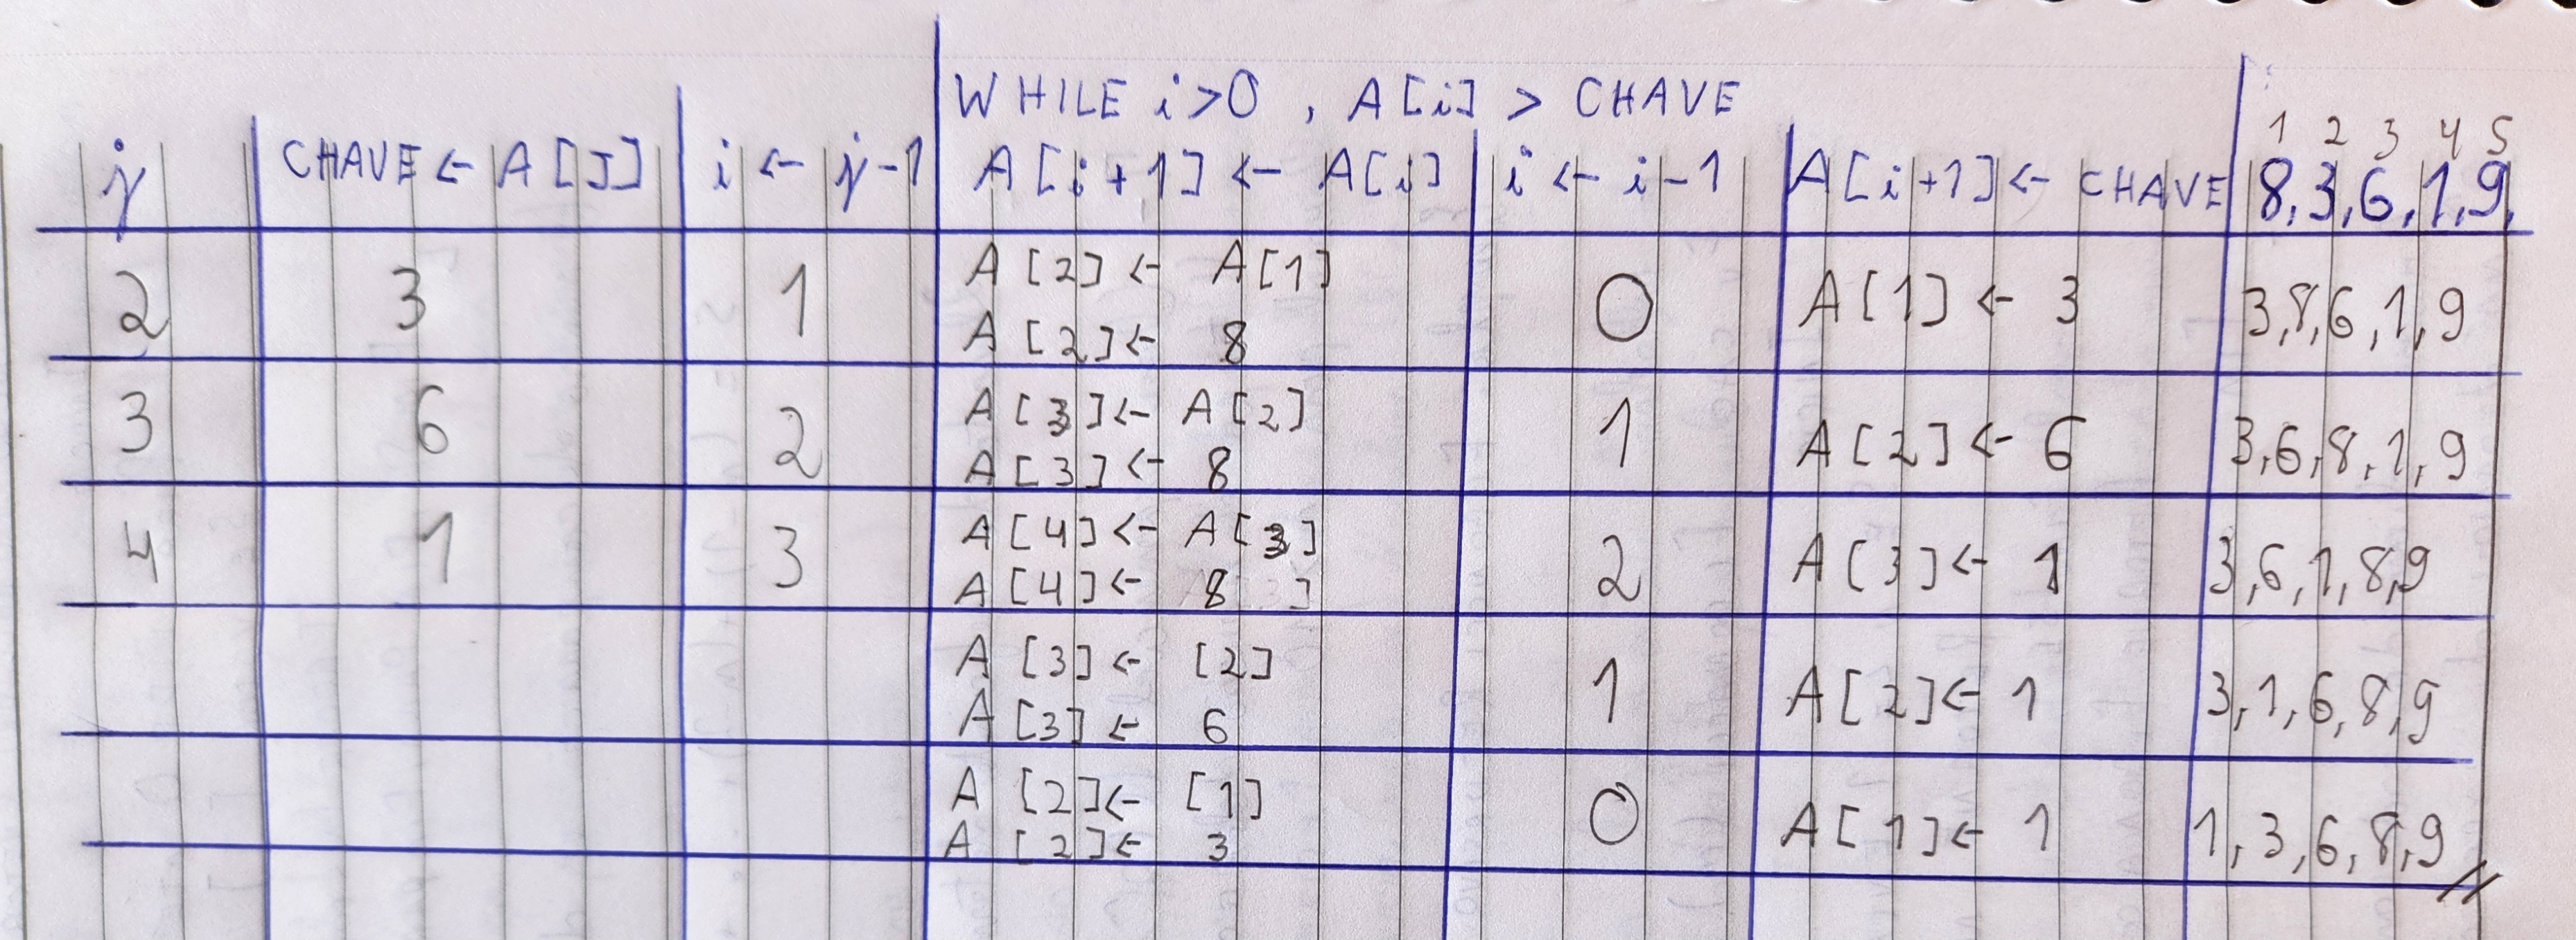
\includegraphics[width=0.9\textwidth]{Imagens/Insertion Sort/teste de mesa.jpeg}
    \caption{Teste de Mesa do algoritmo Insertion Sort (elaborado pelo autor).}
    \label{fig:insertion_mesa}
\end{figure}

\vspace{0.5cm}
\noindent\textbf{Análise Matemática de Complexidade}

\qquad A avaliação de complexidade, fundamentada na literatura clássica da área \cite{cormen}, baseia-se na tabela de custos e frequências apresentada na seção anterior. O desenvolvimento algébrico demonstrado nas Figuras \ref{fig:melhor_caso_math}, \ref{fig:pior_caso_math} e \ref{fig:medio_caso_math} elucida as variações de desempenho do algoritmo conforme a disposição inicial dos dados.

\qquad No \textbf{melhor caso} (Figura \ref{fig:melhor_caso_math}), o vetor de entrada já se encontra ordenado de forma crescente. Consequentemente, a condição do laço de repetição \texttt{while} nunca é satisfeita. O algoritmo realiza apenas uma iteração externa por elemento para verificação, ausentando-se de trocas. Esse comportamento resulta em um tempo de execução de crescimento linear, denotado por $O(n)$.

\begin{figure}[htbp]
    \centering
    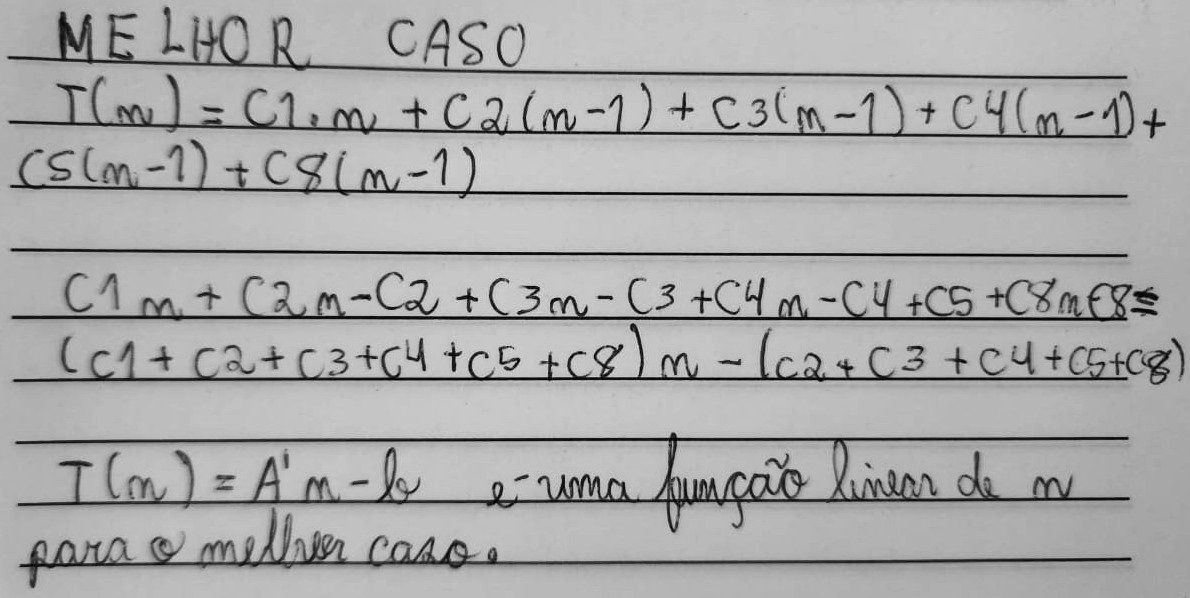
\includegraphics[width=0.6\textwidth]{Imagens/Insertion Sort/melhor caso.jpg}
    \caption{Desenvolvimento matemático da função de tempo para o Melhor Caso (elaborado pelo autor).}
    \label{fig:melhor_caso_math}
\end{figure}

\qquad O \textbf{pior caso} (Figura \ref{fig:pior_caso_math}) representa o cenário diametralmente oposto, em que o vetor está em ordem decrescente. Para cada nova chave avaliada, o algoritmo realiza o número máximo de comparações com a porção já ordenada, exigindo o deslocamento de todos os elementos precedentes. Tal comportamento gera uma quantidade massiva de operações, caracterizando um tempo de execução de crescimento quadrático ($O(n^2)$), o que o torna ineficiente para entradas extensas.

\begin{figure}[htbp]
    \centering
    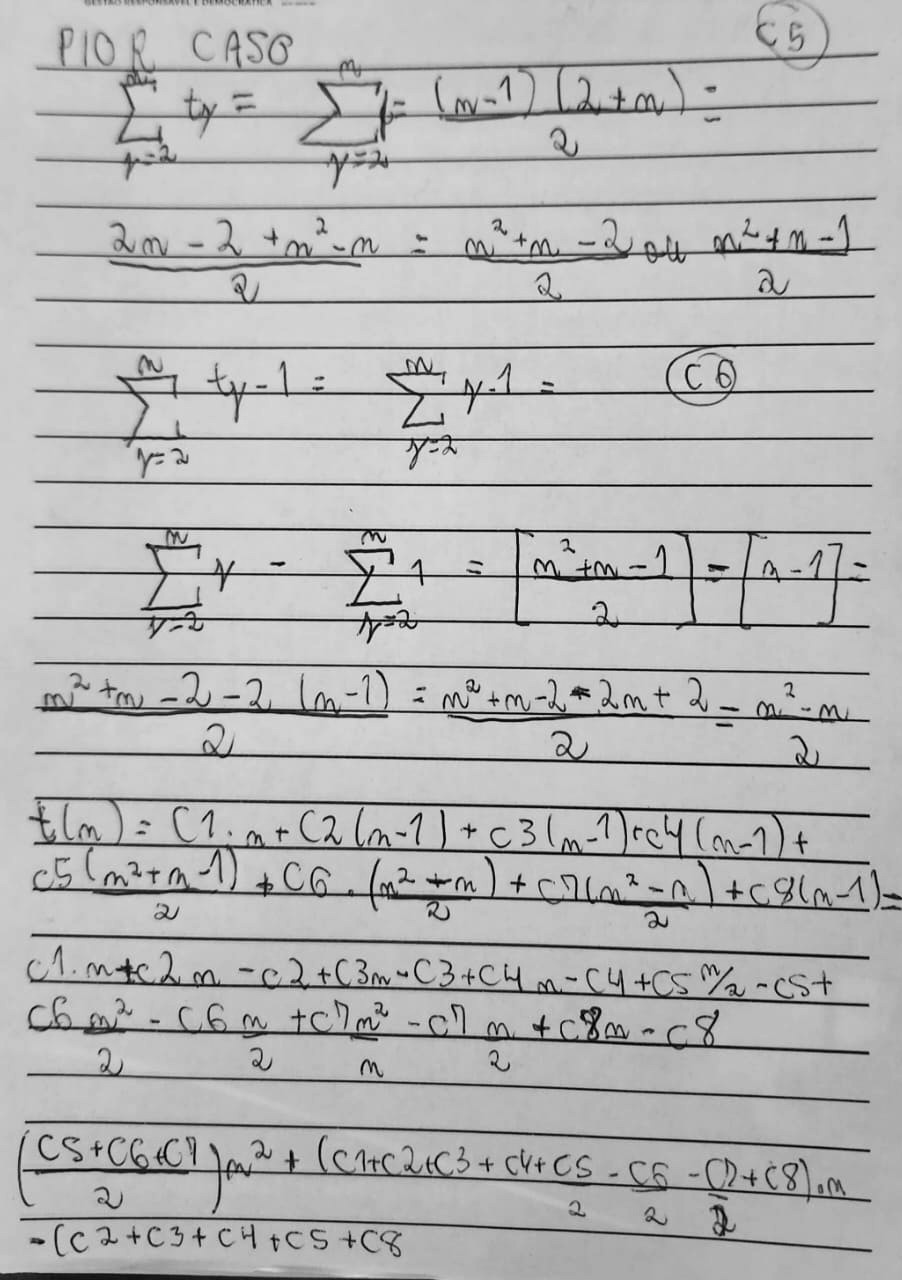
\includegraphics[width=0.7\textwidth]{Imagens/Insertion Sort/pior caso.jpg}
    \caption{Desenvolvimento matemático da função de tempo para o Pior Caso (elaborado pelo autor).}
    \label{fig:pior_caso_math}
\end{figure}

\qquad O \textbf{caso médio} (Figura \ref{fig:medio_caso_math}) ocorre quando os dados estão distribuídos de maneira aleatória. Em termos probabilísticos, o algoritmo necessita percorrer e deslocar, em média, metade dos elementos do subvetor ordenado para encontrar a posição correta de inserção. Embora o número absoluto de operações seja inferior ao do pior caso, o comportamento assintótico da função de tempo mantém o crescimento quadrático ($O(n^2)$).

\begin{figure}[htbp]
    \centering
    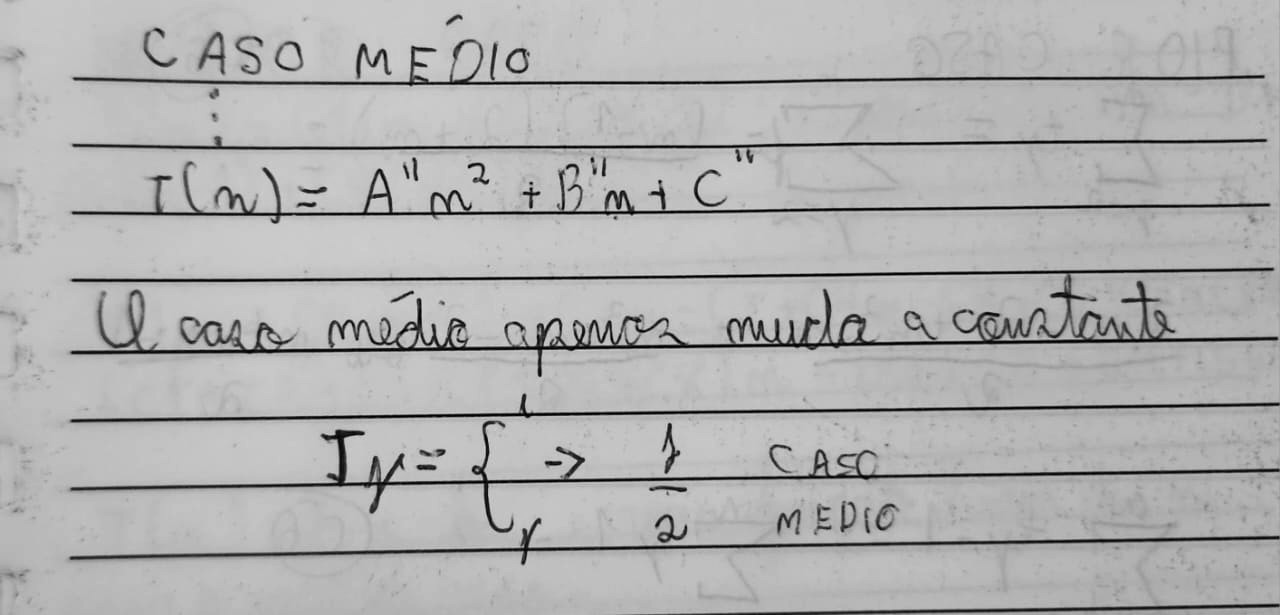
\includegraphics[width=0.8\textwidth]{Imagens/Insertion Sort/caso medio.jpg}
    \caption{Análise da função de tempo para o Caso Médio (elaborado pelo autor).}
    \label{fig:medio_caso_math}
\end{figure}

\qquad Por fim, destaca-se a eficiência espacial do \textit{Insertion Sort}. A quantidade de memória adicional requerida independe do tamanho da entrada, resultando em uma complexidade de espaço $O(1)$. Essa característica é garantida pela ordenação direta no próprio vetor original, configurando uma operação \textit{in-place}.
	    \vspace*{1.5cm}
		\subsection{Bubble Sort}
		% --- CÓDIGO ATUALIZADO para Analise/bubble_sort_analise.tex ---

\subsubsection*{Análise de Complexidade e Teste de Mesa - Bubble Sort}

\qquad Esta seção apresenta o teste de mesa do \textit{Bubble Sort} e a derivação de sua função de tempo $T(n)$.

\paragraph{Teste de Mesa}
\qquad A Figura \ref{fig:bubble_mesa} mostra a execução do \textit{Bubble Sort}, acompanhando os valores das variáveis \texttt{i} e \texttt{j} e o estado do vetor a cada comparação e troca. É possível observar o maior elemento sendo deslocado para o final do vetor a cada passagem do laço externo.

% --- IMAGEM DO TESTE DE MESA ---
\begin{figure}[htbp]
    \centering
    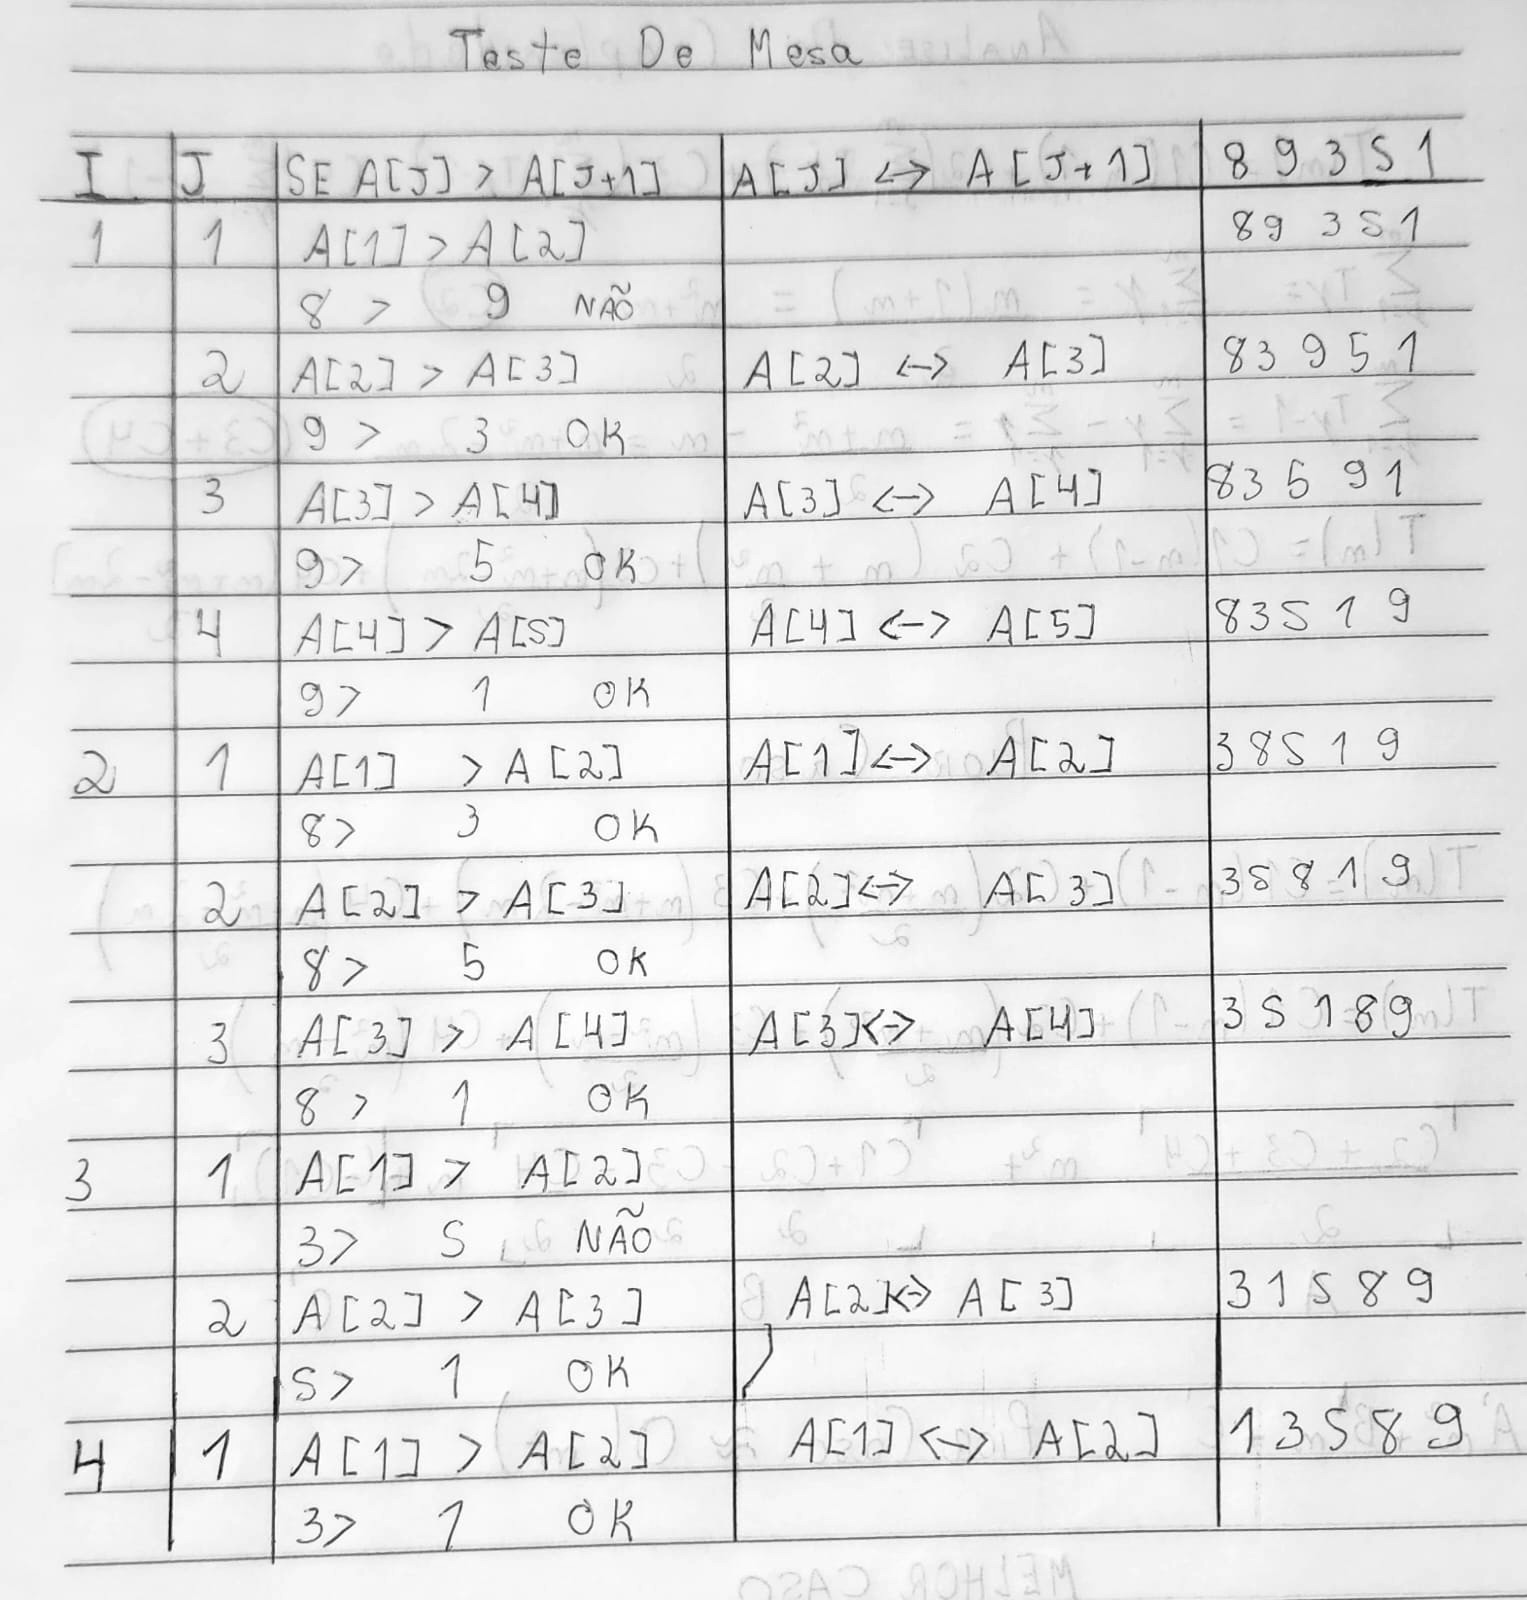
\includegraphics[width=1.0\textwidth]{Imagens/Bubble Sort/testedemesa-bubble.jpg}
    \caption{Teste de Mesa do algoritmo Bubble Sort (elaborado pelo autor).}
    \label{fig:bubble_mesa}
\end{figure}

\paragraph{Análise Matemática Geral}
\qquad A Figura \ref{fig:bubble_analise_geral} apresenta a dedução da função de tempo $T(n)$ a partir da tabela de custos e da frequência de execução dos laços aninhados.

% --- IMAGEM DA ANÁLISE DE COMPLEXIDADE GERAL ---
\begin{figure}[htbp]
    \centering
    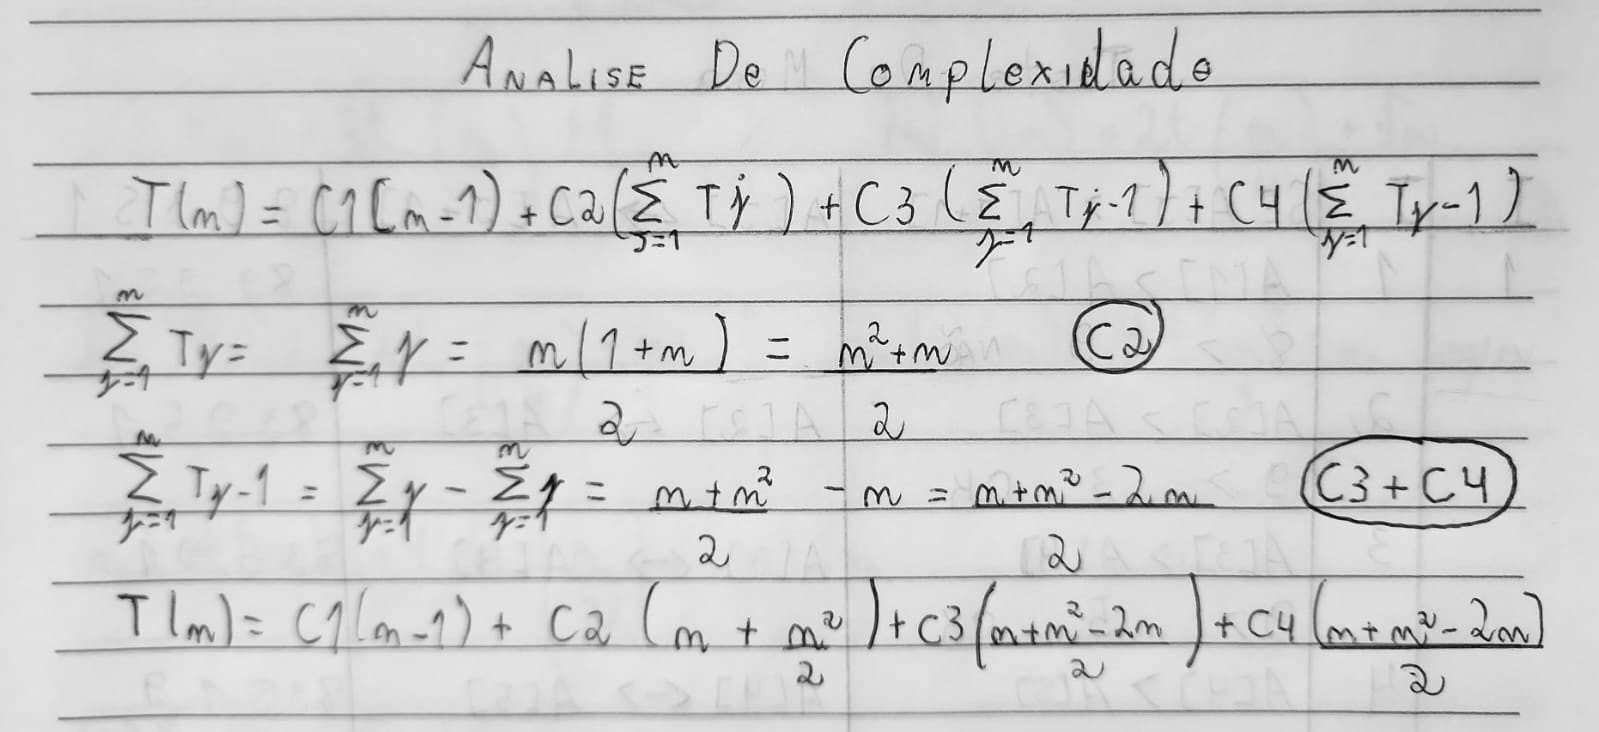
\includegraphics[width=1.0\textwidth]{Imagens/Bubble Sort/analisedecomplexidade-bubble.jpg}
    \caption{Análise de Complexidade geral do Bubble Sort (elaborado pelo autor).}
    \label{fig:bubble_analise_geral}
\end{figure}


\paragraph{Análise por Cenário}
\qquad A seguir, a função de tempo é analisada separadamente para os três cenários: melhor, pior e médio caso.

\qquad No \textbf{melhor caso} (Figura \ref{fig:bubble_melhor_math}), mesmo sem a necessidade de trocas, a implementação ainda percorre os laços por completo, o que mantém a complexidade em $O(n^2)$.

% --- IMAGEM DO MELHOR CASO ---
\begin{figure}[htbp]
    \centering
    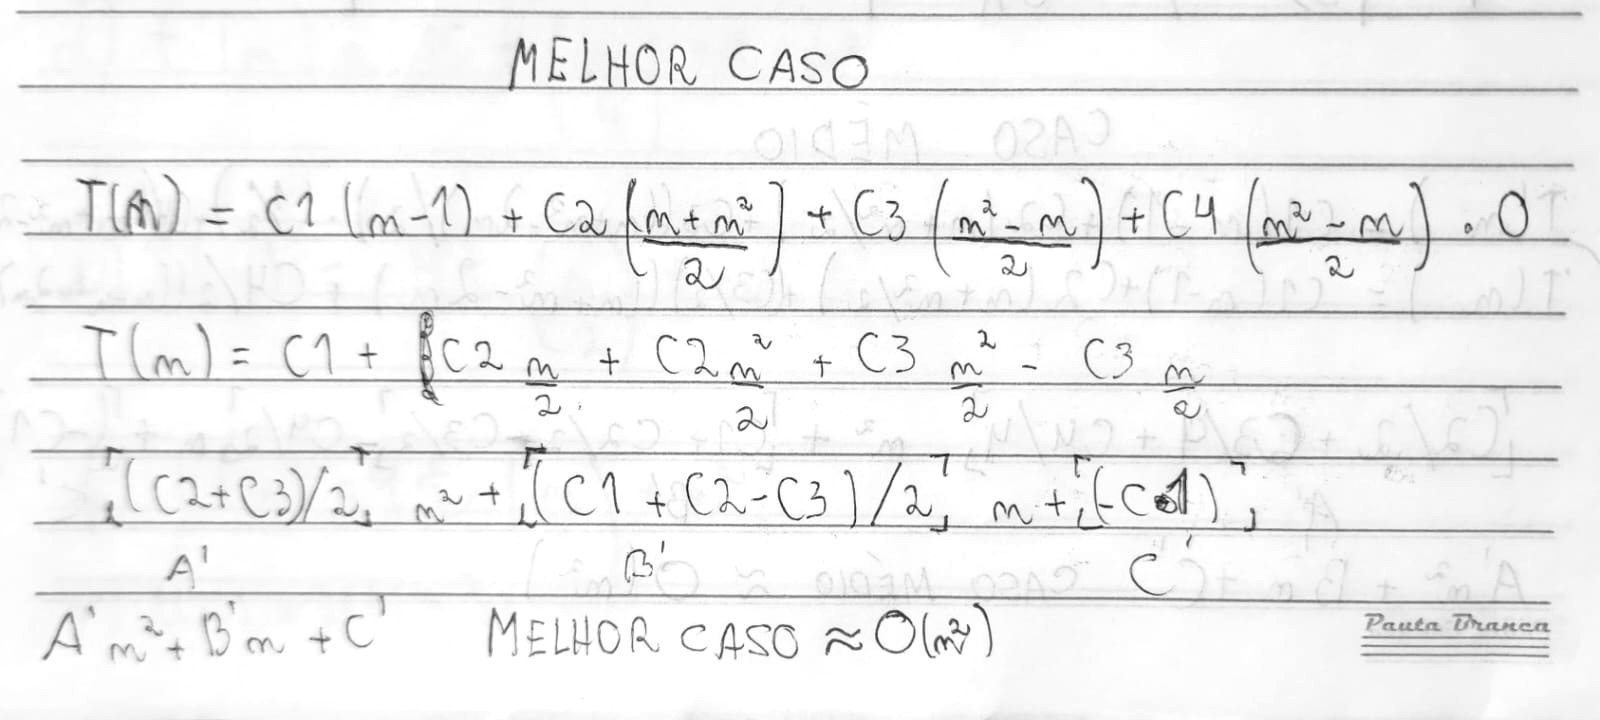
\includegraphics[width=0.9\textwidth]{Imagens/Bubble Sort/melhorcaso-bubble.jpg}
    \caption{Desenvolvimento matemático para o Melhor Caso do Bubble Sort (elaborado pelo autor).}
    \label{fig:bubble_melhor_math}
\end{figure}

\qquad No \textbf{pior caso} (Figura \ref{fig:bubble_pior_math}), com o vetor em ordem inversa, ocorre o número máximo de trocas, o que também resulta em $O(n^2)$.

% --- IMAGEM DO PIOR CASO ---
\begin{figure}[htbp]
    \centering
    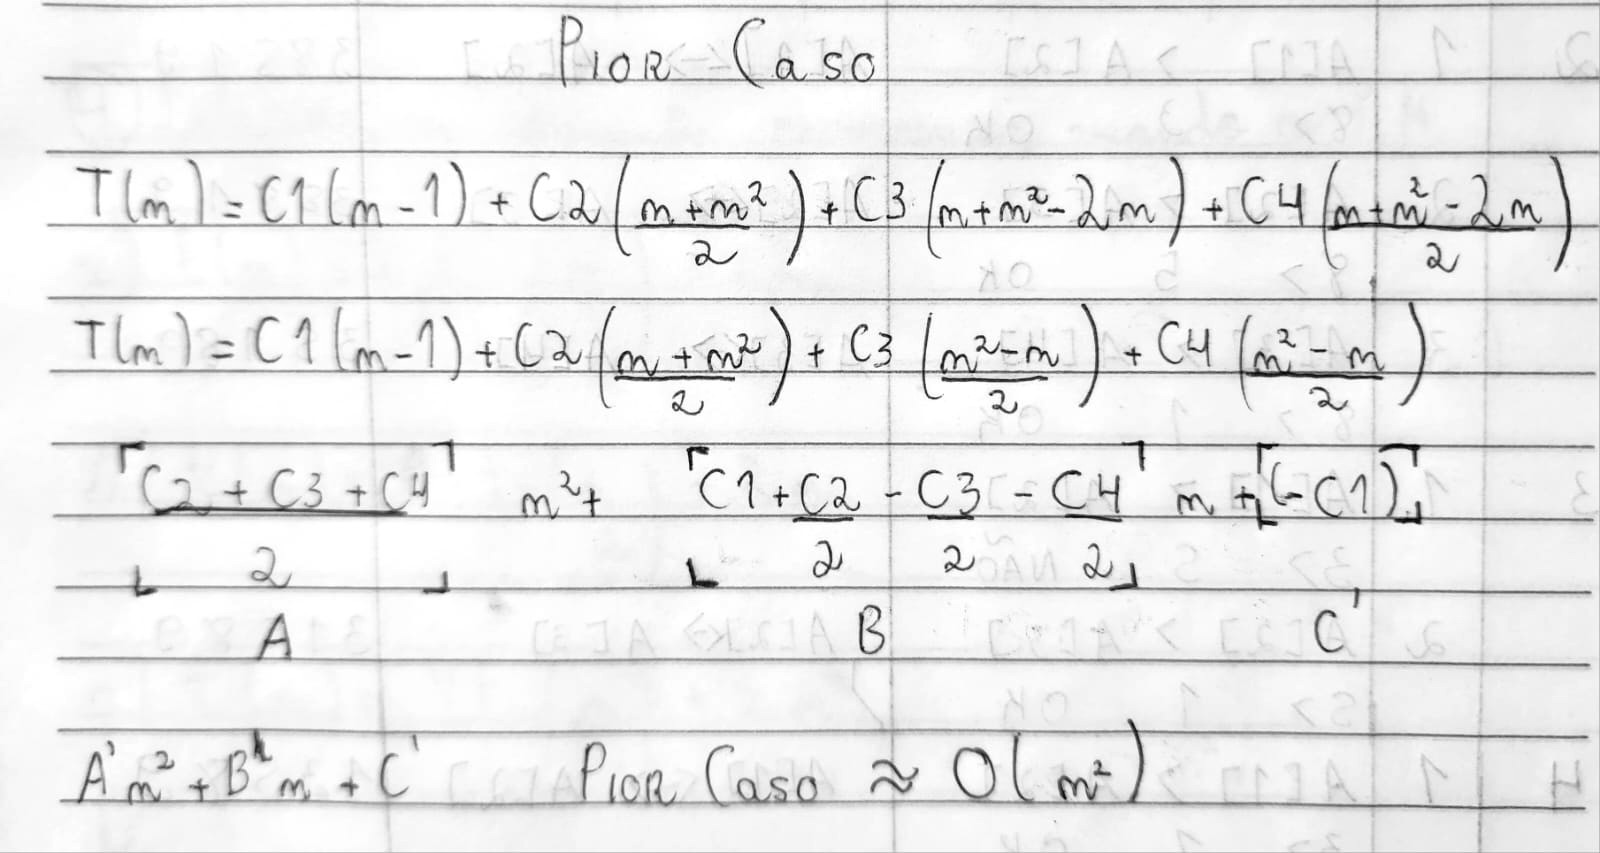
\includegraphics[width=0.9\textwidth]{Imagens/Bubble Sort/piorcaso-bubble.jpg}
    \caption{Desenvolvimento matemático para o Pior Caso do Bubble Sort (elaborado pelo autor).}
    \label{fig:bubble_pior_math}
\end{figure}

\qquad No \textbf{caso médio} (Figura \ref{fig:bubble_medio_math}), o número de comparações continua sendo o fator dominante, o que resulta na mesma complexidade $O(n^2)$.

% --- IMAGEM DO CASO MÉDIO ---
\begin{figure}[htbp]
    \centering
    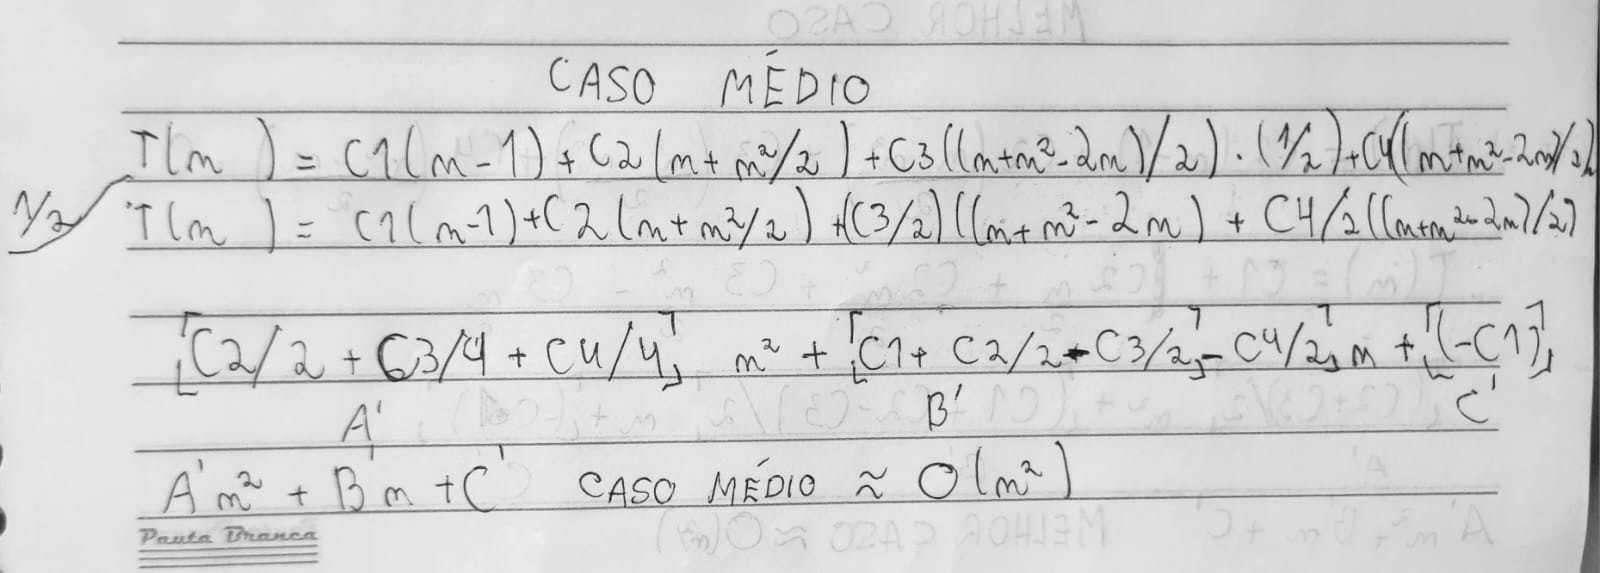
\includegraphics[width=0.9\textwidth]{Imagens/Bubble Sort/mediocaso-bubble.jpg}
    \caption{Análise da função de tempo para o Caso Médio do Bubble Sort (elaborado pelo autor).}
    \label{fig:bubble_medio_math}
\end{figure}

\FloatBarrier

\qquad Quanto à \textbf{complexidade de espaço}, o \textit{Bubble Sort} apresenta complexidade $O(1)$, já que a ordenação é feita \textit{in-place}, sem uso de estruturas auxiliares proporcionais a $n$.
	    \vspace*{1.5cm}
		\subsection{Selection Sort}
		% --- CÓDIGO ATUALIZADO para Analise/selection_sort_analise.tex ---

\subsubsection*{Análise de Complexidade e Teste de Mesa - Selection Sort}

\qquad Esta seção apresenta o teste de mesa do \textit{Selection Sort}, a derivação de sua função de tempo $T(n)$ e a análise de cada cenário.

\paragraph{Teste de Mesa}
\qquad A Figura \ref{fig:selection_mesa} mostra a execução do \textit{Selection Sort}, acompanhando o estado do vetor e das variáveis a cada passo do algoritmo na busca pelo menor elemento e seu posicionamento correto.

% --- IMAGEM DO TESTE DE MESA ---
\begin{figure}[htbp]
    \centering
    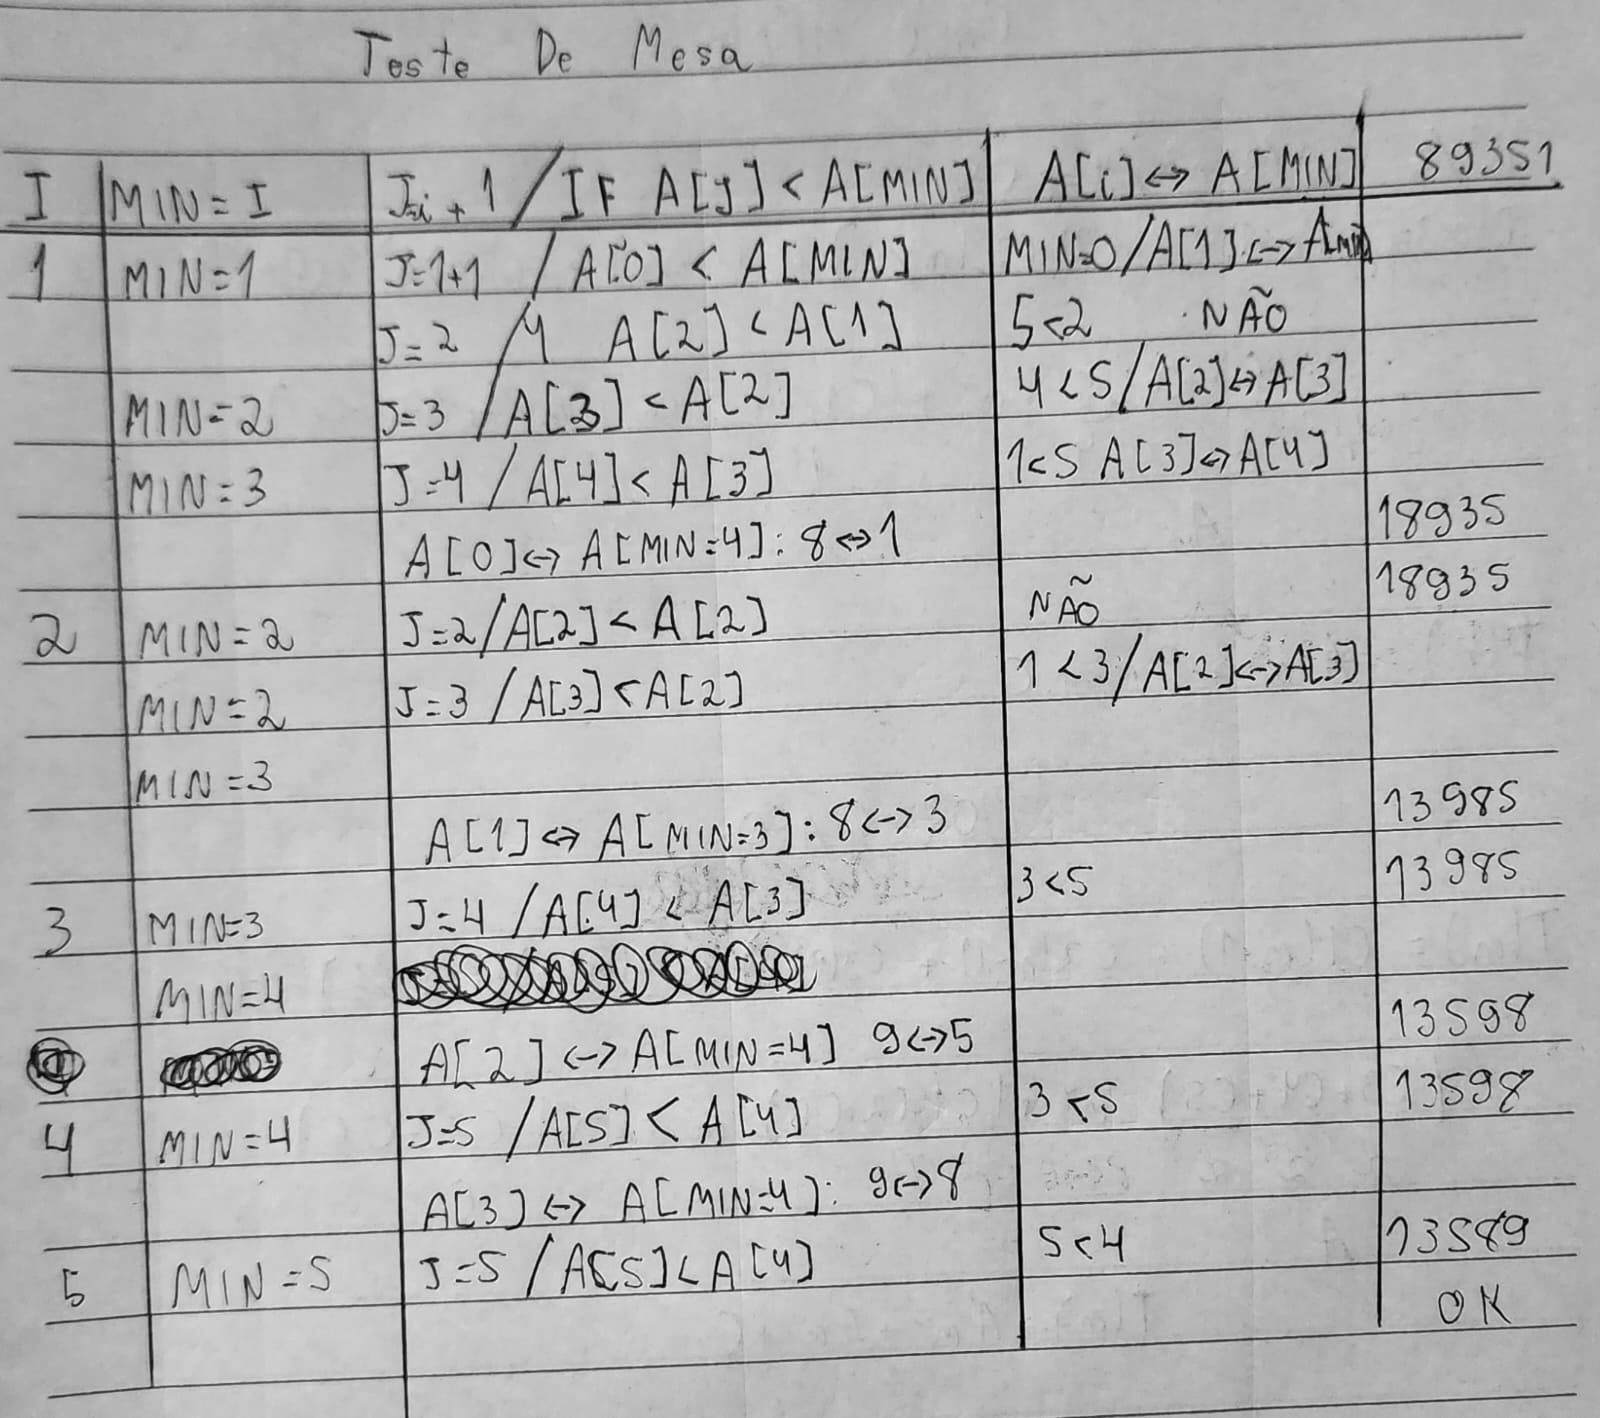
\includegraphics[width=1.0\textwidth]{Imagens/Selection Sort/testedemesa-selection.jpg}
    \caption{Teste de Mesa do algoritmo Selection Sort (elaborado pelo autor).}
    \label{fig:selection_mesa}
\end{figure}

\paragraph{Análise Matemática de Complexidade (Escrita)}
\qquad A função de tempo total, $T(n)$, é dada pela soma do custo de cada linha ($c_i$) multiplicado pelo número de vezes que ela é executada. Com base na tabela de custos apresentada na seção de Algoritmos, a equação geral é:
$$ T(n) = c_1(1) + c_2(n) + c_3(n-1) + c_4\left(\frac{n(n-1)}{2}\right) + c_5\left(\frac{n(n-1)}{2}\right) + c_6(\text{soma}) + c_7(n-1) $$
\qquad Agrupando os termos por potência de $n$, o termo dominante é proporcional a $n^2$, originado pelos laços aninhados:
$$ T(n) = \left(\frac{c_4+c_5}{2}\right)n^2 + \dots $$
\qquad Assim, a função de tempo do \textit{Selection Sort} é sempre quadrática, na forma $An^2 + Bn + C$. A única variação entre os cenários está no valor da "soma" (custo $c_6$, referente às atualizações de \texttt{min\_idx}), que não influencia o termo dominante. Por isso, a complexidade é $O(n^2)$ em todos os casos.


\paragraph{Análise por Cenário (com Imagens)}
\qquad A seguir, o resultado dessa análise é detalhado para cada cenário.

\qquad No \textbf{melhor caso} (Figura \ref{fig:selection_melhor_math}), mesmo com o vetor já ordenado, a complexidade permanece $O(n^2)$, já que todas as comparações são realizadas independentemente da ordem inicial dos elementos.

% --- IMAGEM DO MELHOR CASO ---
\begin{figure}[htbp]
    \centering
    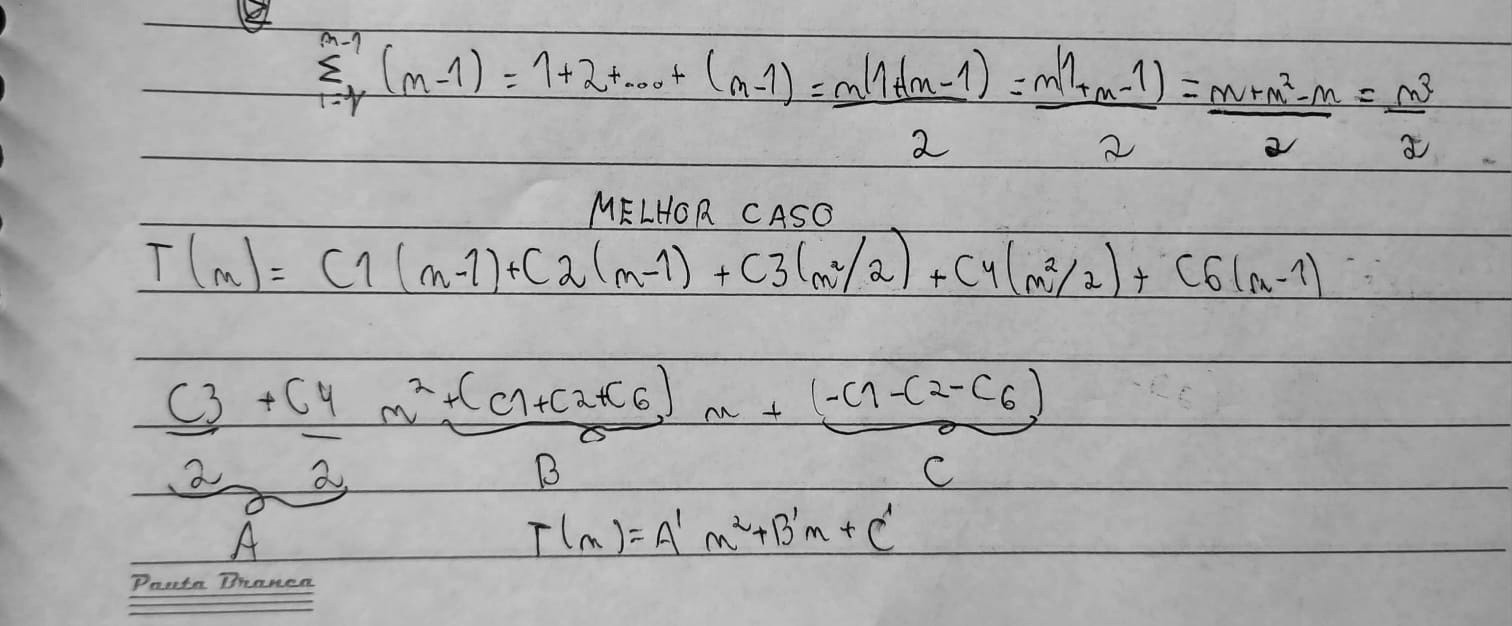
\includegraphics[width=0.9\textwidth]{Imagens/Selection Sort/melhorcaso-selection.jpg}
    \caption{Análise manuscrita para o Melhor Caso do Selection Sort (elaborado pelo autor).}
    \label{fig:selection_melhor_math}
\end{figure}

\qquad No \textbf{pior caso} (Figura \ref{fig:selection_pior_math}), com o vetor em ordem inversa, o número de comparações não se altera, mantendo a mesma complexidade $O(n^2)$.

% --- IMAGEM DO PIOR CASO ---
\begin{figure}[htbp]
    \centering
    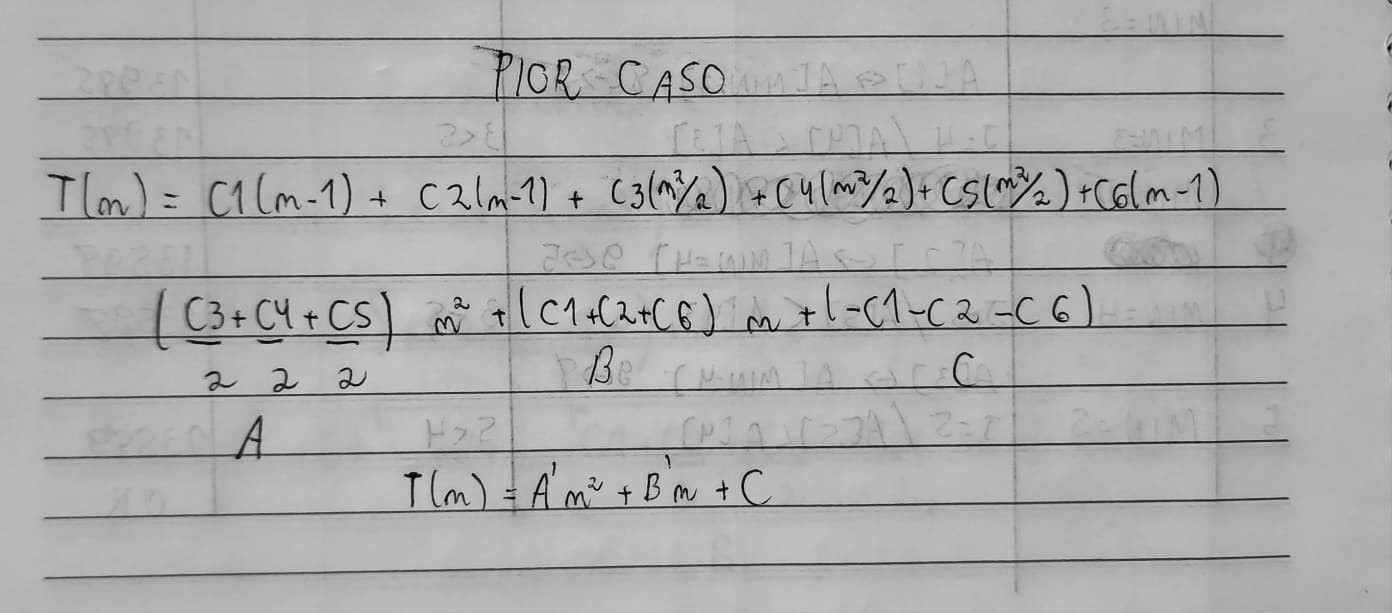
\includegraphics[width=0.9\textwidth]{Imagens/Selection Sort/piorcaso-selection.jpg}
    \caption{Análise manuscrita para o Pior Caso do Selection Sort (elaborado pelo autor).}
    \label{fig:selection_pior_math}
\end{figure}

\qquad No \textbf{caso médio} (Figura \ref{fig:selection_medio_math}), o resultado é o mesmo, com complexidade $O(n^2)$.

% --- IMAGEM DO CASO MÉDIO ---
\begin{figure}[htbp]
    \centering
    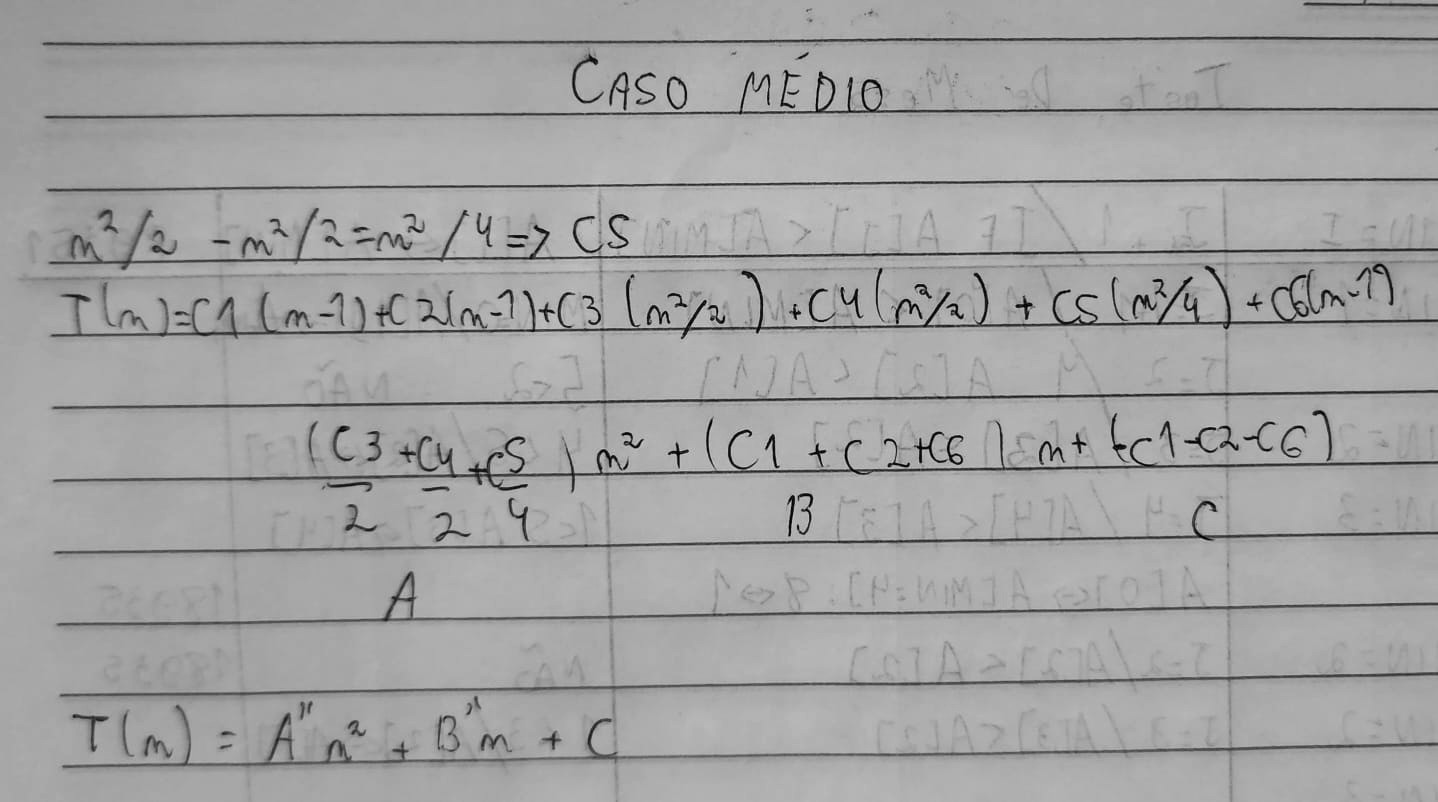
\includegraphics[width=0.9\textwidth]{Imagens/Selection Sort/mediocaso-selection.jpg}
    \caption{Análise manuscrita para o Caso Médio do Selection Sort (elaborado pelo autor).}
    \label{fig:selection_medio_math}
\end{figure}

\FloatBarrier

\qquad Quanto à \textbf{complexidade de espaço}, o \textit{Selection Sort} apresenta complexidade $O(1)$, pois a ordenação é feita \textit{in-place}, sem uso de estruturas auxiliares proporcionais a $n$.
	    \vspace*{1.5cm}
		\subsection{Shell Sort}
		% --- CÓDIGO ATUALIZADO para Analise/shell_sort_analise.tex ---

\subsubsection*{Análise e Interpretação dos Resultados - Shell Sort}

\qquad A análise exata do \textit{Shell Sort} é mais complexa que a dos demais algoritmos deste trabalho, pois seu desempenho depende diretamente da sequência de intervalos (\textit{gaps}) utilizada. A análise apresentada a seguir considera a implementação com a sequência $n/2, n/4, \dots, 1$ e se baseia nos resultados já estabelecidos na literatura \cite{sedgewick}.

\qquad Os principais casos de desempenho para essa sequência de \textit{gaps} são os seguintes:
\begin{itemize}
    \item \textbf{Melhor caso:} ocorre quando o vetor já está ordenado. O laço externo dos \textit{gaps} executa aproximadamente $\log n$ vezes e, como nenhum deslocamento é necessário, o laço interno percorre o vetor realizando apenas comparações. Isso resulta em complexidade $O(n \log n)$.

    \item \textbf{Pior caso:} para a sequência de \textit{gaps} utilizada no código, o pior caso conhecido é $O(n^2)$. Existem arranjos específicos de dados que levam o algoritmo a esse desempenho.

    \item \textbf{Caso médio:} não há uma fórmula fechada para essa sequência de \textit{gaps}. As estimativas mais aceitas indicam uma complexidade subquadrática, em torno de $O(n^{1,5})$. Na prática, o que importa é que o desempenho médio fica bem abaixo de $O(n^2)$.
\end{itemize}

\qquad Para ilustrar de forma concreta o funcionamento do algoritmo, a Figura \ref{fig:shell_teste_mesa} apresenta um teste de mesa realizado com essa mesma sequência de \textit{gaps}, mostrando passo a passo como o vetor se aproxima da ordenação a cada passagem.

% --- IMAGEM ÚNICA PARA A ANÁLISE GERAL ---
\begin{figure}[htbp]
    \centering
    % ATENÇÃO: Faça o upload da sua imagem do teste de mesa com este nome ou altere aqui
    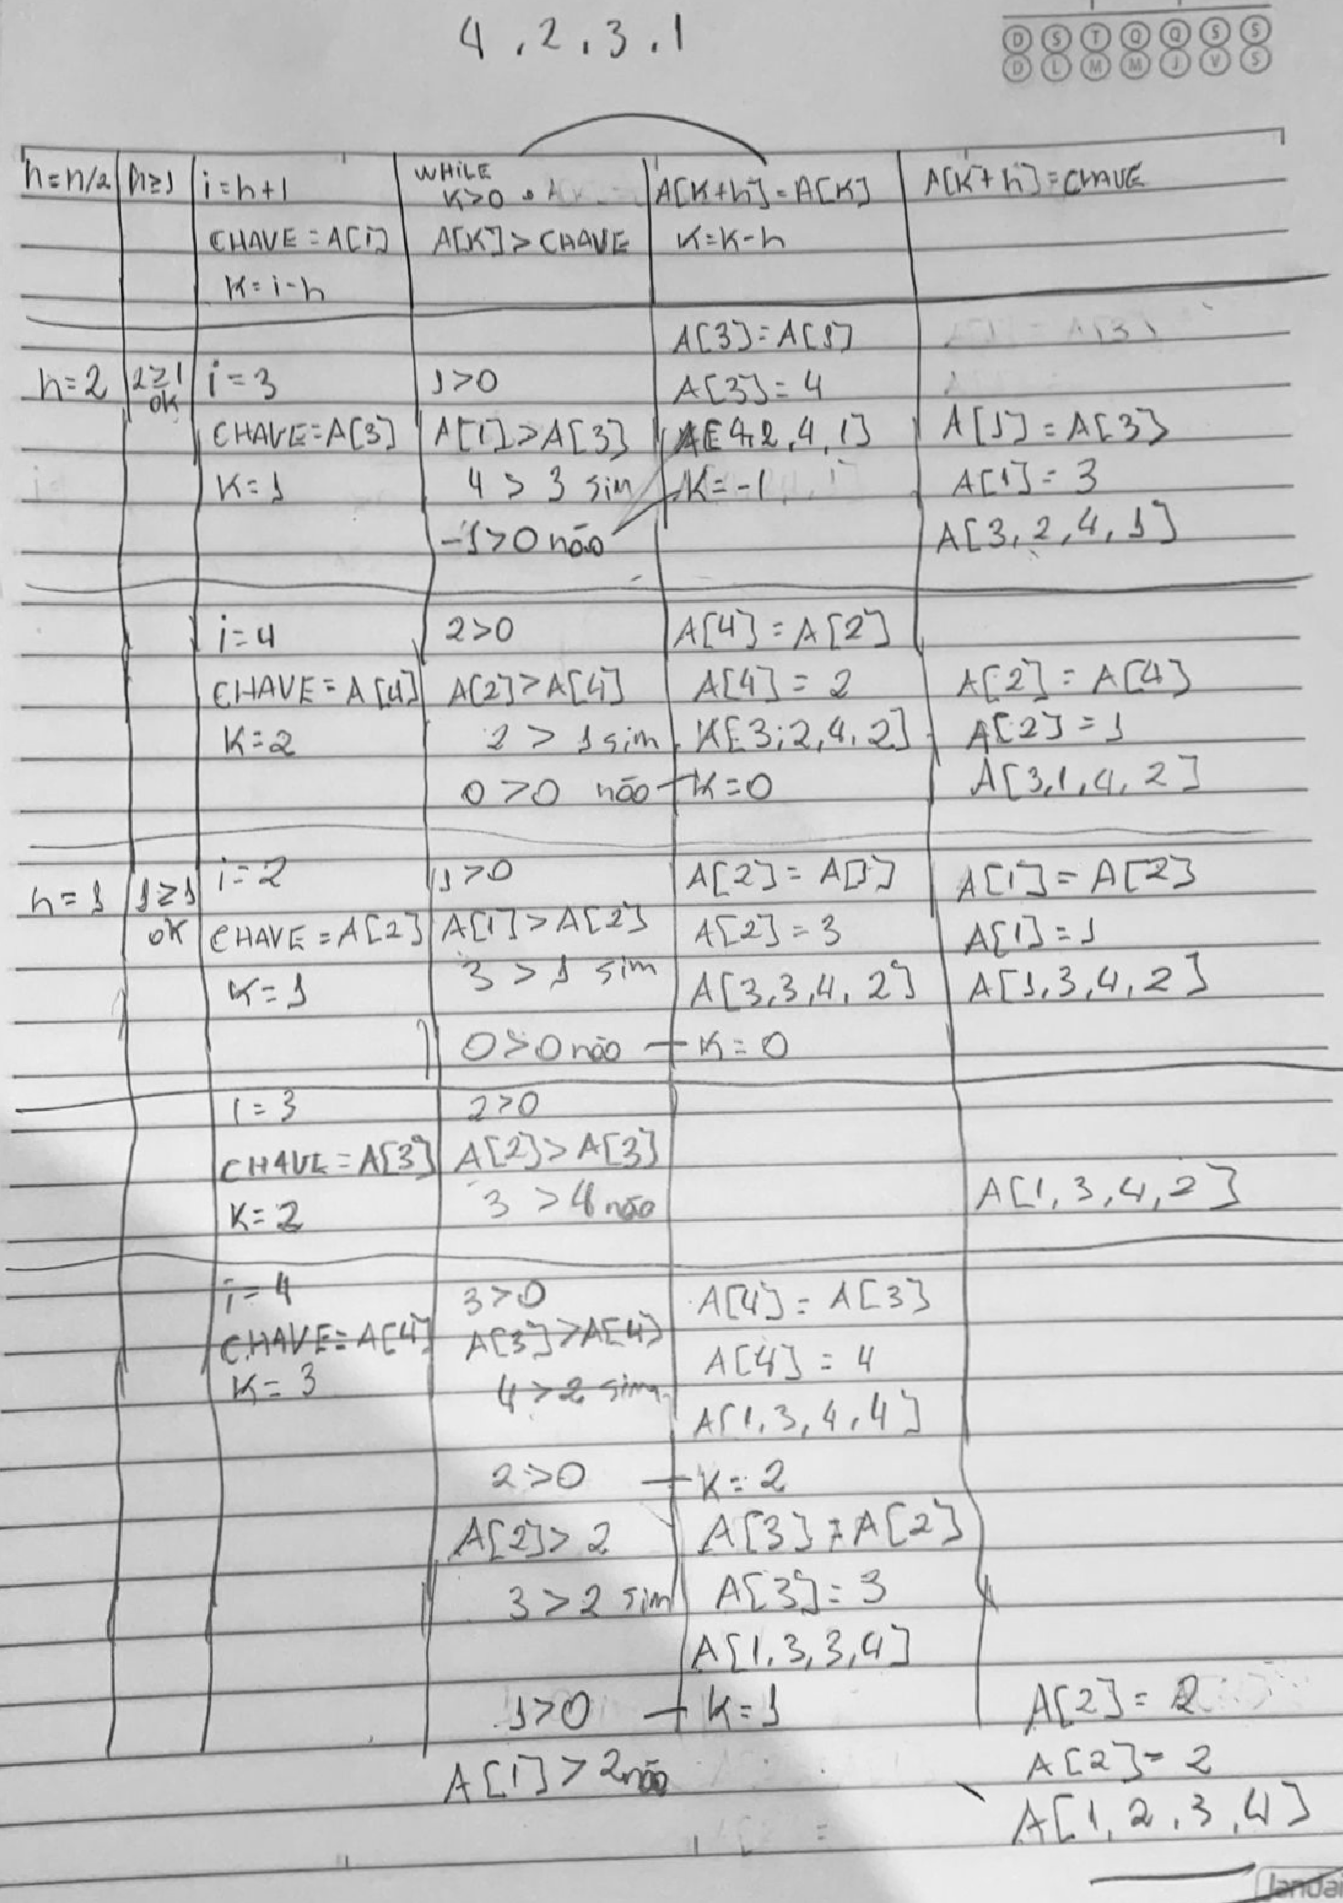
\includegraphics[width=0.9\textwidth]{Imagens/Shell_sort/TesteDeMesa.png}
    \caption{Teste de mesa do Shell Sort com a sequência de \textit{gaps} $n/2, n/4, \dots, 1$ (elaborado pelo autor).}
    \label{fig:shell_teste_mesa}
\end{figure}

\FloatBarrier

\qquad Os tempos medidos nos testes são compatíveis com essa análise: ao aumentar a entrada de 100.000 para 1.000.000 de elementos, o tempo do caso aleatório cresceu cerca de 15 vezes, enquanto em um algoritmo quadrático o crescimento esperado seria de aproximadamente 100 vezes.

\qquad Quanto à \textbf{complexidade de espaço}, o \textit{Shell Sort} apresenta complexidade $O(1)$, pois a ordenação é feita \textit{in-place}, sem uso de estruturas auxiliares proporcionais a $n$.
	    \vspace*{1.5cm}
        \subsection{Merge Sort}
		\subsubsection*{Análise e Interpretação dos Resultados - Merge Sort}

\qquad A análise do \textit{Merge Sort} é mais direta que a dos algoritmos anteriores, pois seu comportamento não depende da ordem inicial dos dados. Em qualquer vetor, o algoritmo divide o trecho ao meio até chegar a elementos individuais e depois intercala as partes. Como o número de divisões e o custo das intercalações são sempre os mesmos, o desempenho é o mesmo nos três casos \cite{sedgewick}.

\qquad Para ilustrar o funcionamento do algoritmo, a Figura \ref{fig:merge_teste_mesa} apresenta um teste de mesa com um vetor de sete elementos. Como o vetor tem tamanho ímpar, a metade esquerda recebe um elemento a mais, o que reflete o cálculo do ponto médio feito no código. A parte superior da figura mostra a divisão e a parte inferior mostra as intercalações.

\begin{figure}[htbp]
    \centering
    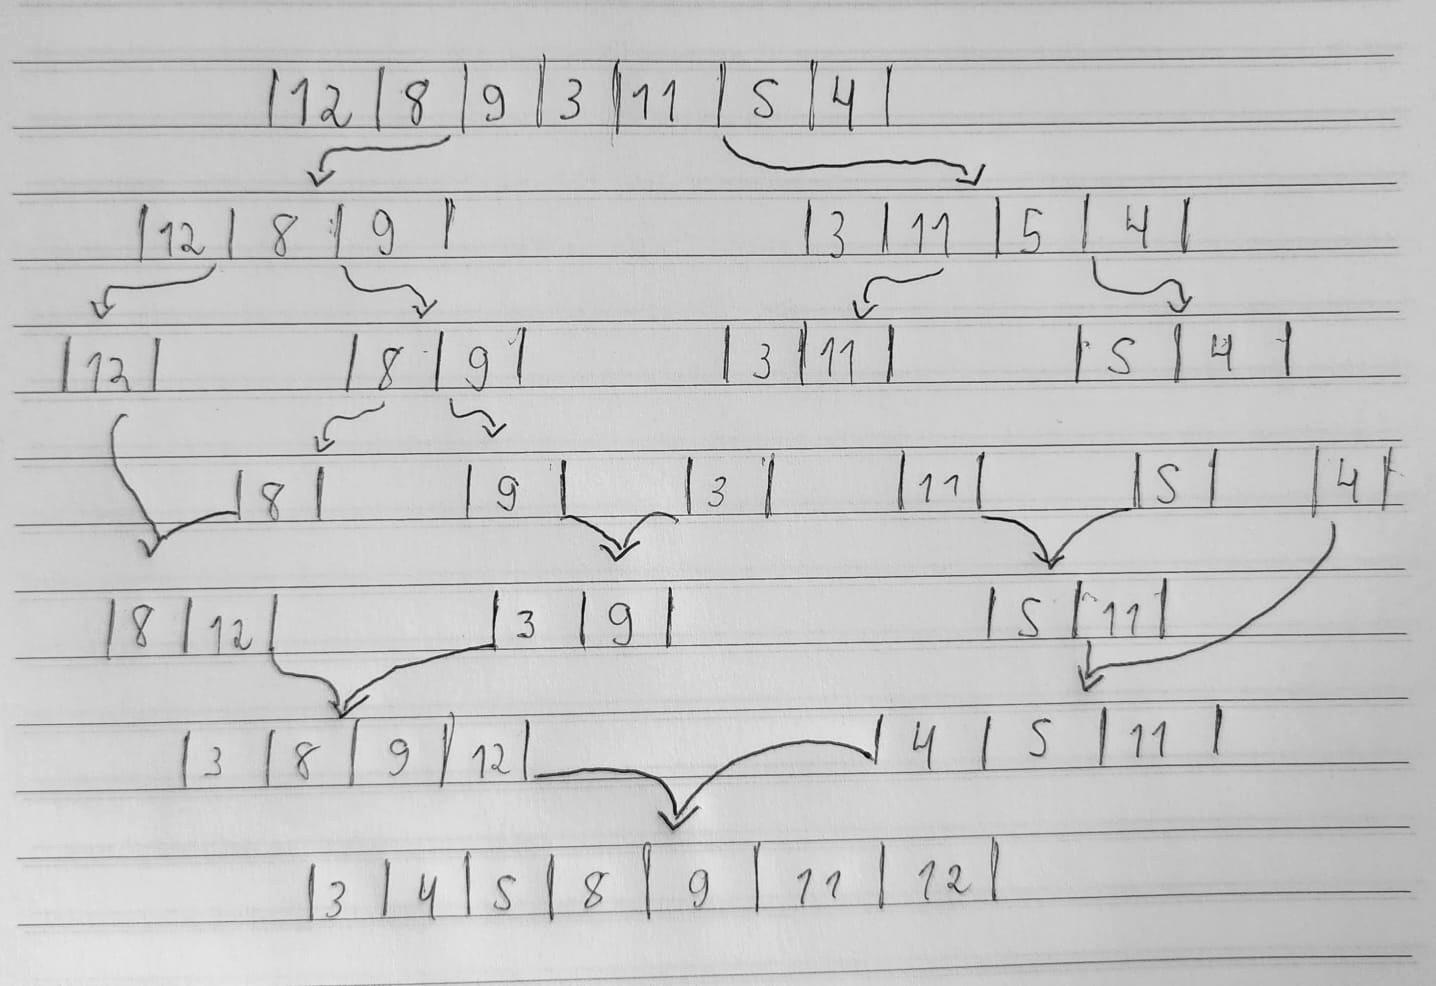
\includegraphics[width=0.9\textwidth]{Imagens/Merge Sort/mergeteste.jpeg}
    \caption{Teste de mesa do \textit{Merge Sort} para um vetor de sete elementos (elaborado pelo autor).}
    \label{fig:merge_teste_mesa}
\end{figure}

\FloatBarrier

\qquad Para obter a complexidade, usa-se a recorrência do algoritmo. O tempo $T(n)$ para ordenar $n$ elementos é a soma do custo constante de calcular o ponto médio, do tempo das duas chamadas recursivas sobre metades do vetor e do custo da intercalação, que é $\Theta(n)$, como visto na análise do código. Isso resulta em $T(n) = 2T(n/2) + n$. A Figura \ref{fig:merge_recorrencia} mostra o desenvolvimento dessa recorrência por expansão, considerando $n = 2^k$.

\begin{figure}[htbp]
    \centering
    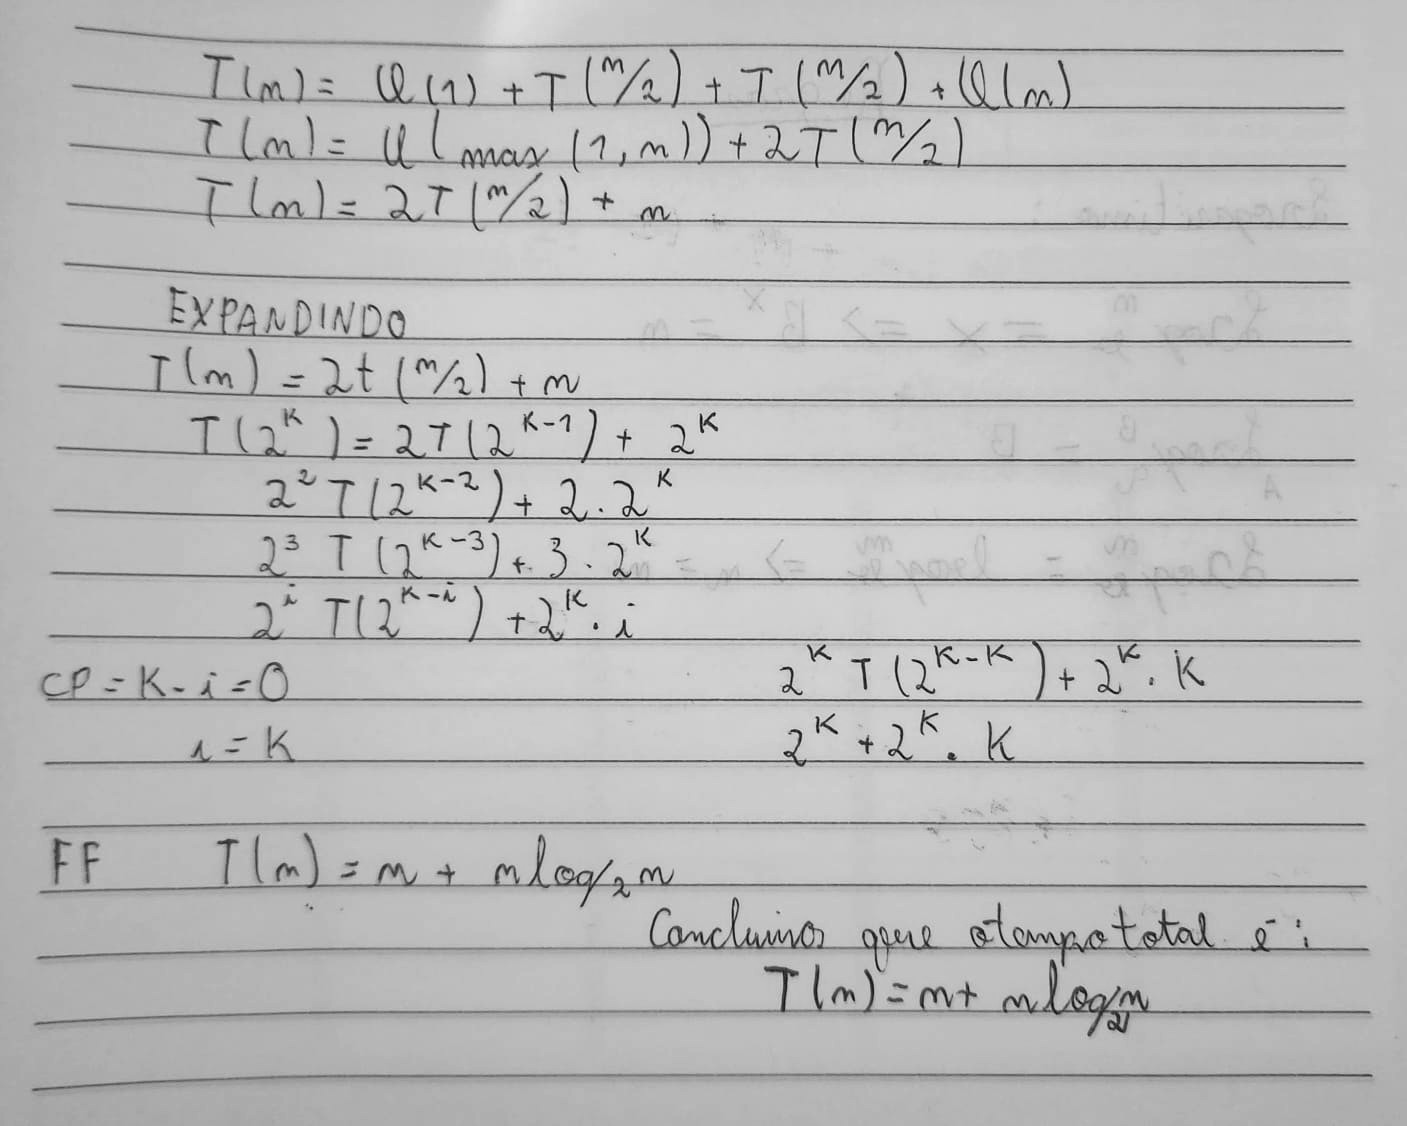
\includegraphics[width=0.8\textwidth]{Imagens/Merge Sort/mergecalculo.jpg}
    \caption{Resolução da recorrência do \textit{Merge Sort} por expansão (elaborado pelo autor).}
    \label{fig:merge_recorrencia}
\end{figure}


\qquad Ao expandir a recorrência, cada nível acrescenta o termo $2^k$ ao custo. Isso acontece porque, a cada nível, o número de subproblemas dobra e o tamanho de cada um cai pela metade, de modo que o total de elementos intercalados por nível continua sendo $n$. A expansão termina quando $k - i = 0$, ou seja, $i = k$, e o resultado é $T(n) = 2^k + 2^k \cdot k$. Como $n = 2^k$, tem-se $k = \log_2 n$, e portanto
\[
T(n) = n + n \log_2 n .
\]
Esse resultado mostra que o tempo total é $O(n \log n)$. Os principais casos de desempenho são:
\begin{itemize}
    \item \textbf{Melhor caso:} $O(n \log n)$. Mesmo com o vetor já ordenado, o algoritmo faz todas as divisões e todas as intercalações, pois não existe verificação que permita interromper o processo mais cedo.

    \item \textbf{Pior caso:} $O(n \log n)$. A altura da árvore de chamadas é sempre $\log_2 n$, e cada nível custa $n$ em qualquer ordem dos dados. Diferente do \textit{Bubble Sort} e do \textit{Selection Sort}, o pior caso não chega a $O(n^2)$.

    \item \textbf{Caso médio:} $O(n \log n)$, pelo mesmo motivo dos casos anteriores.
\end{itemize}

\qquad Os tempos medidos nos testes são compatíveis com essa análise. Ao aumentar a entrada de 100.000 para 1.000.000 de elementos (10 vezes maior), o tempo do caso aleatório passou de 0,023 para 0,292, um crescimento de cerca de 12,7 vezes. Para $n \log n$, o crescimento esperado nessa mudança é de aproximadamente 12 vezes, enquanto em um algoritmo quadrático seria de 100 vezes. Nos vetores crescentes e decrescentes o crescimento foi de cerca de 11 e 9 vezes, respectivamente. Os tempos dos três tipos de entrada ficaram próximos entre si, o que confirma que o \textit{Merge Sort} não depende da ordem inicial dos dados. A diferença entre eles vem de detalhes de execução, como o número de comparações feitas em cada intercalação e o uso do \textit{cache} do processador.

\qquad Quanto à \textbf{complexidade de espaço}, o \textit{Merge Sort} utiliza $O(n)$, devido ao vetor auxiliar de $n$ posições usado nas intercalações, além de $O(\log n)$ para a pilha de chamadas recursivas. Por isso, diferente dos demais algoritmos deste trabalho, ele não é \textit{in-place}. Em troca desse espaço extra, ele garante o desempenho $O(n \log n)$ em todos os casos e é estável.
	    \vspace*{1.5cm}
        
		\section{TABELA E GRÁFICO}
            \subsection{Insertion Sort}
		\subsection*{Resultados Empíricos - Insertion Sort}

\qquad Os testes experimentais foram executados com vetores de tamanhos variando de $n = 10$ a $n = 1.000.000$ elementos, sob três configurações de entrada: crescente (melhor caso), decrescente (pior caso) e aleatória (caso médio). A Tabela \ref{tab:insertion_tempos} apresenta a compilação dos tempos de execução aferidos em segundos.

\begin{table}[htbp]
    \centering
    \caption{Tempo de execução (em segundos) do Insertion Sort para diferentes tamanhos de entrada.}
    \label{tab:insertion_tempos}
    \vspace{0.2cm}
    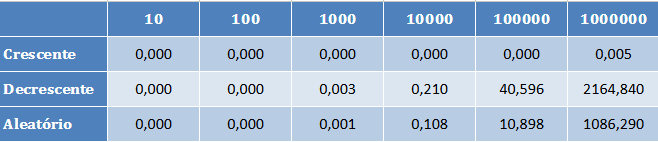
\includegraphics[width=0.9\textwidth]{Imagens/Insertion Sort/tabela insertion.png}
\end{table}

\qquad A representação gráfica do desempenho do algoritmo é ilustrada na Figura \ref{fig:insertion_grafico}. A curva observada valida diretamente a modelagem matemática assintótica desenvolvida nas seções anteriores.

\begin{figure}[htbp]
    \centering
    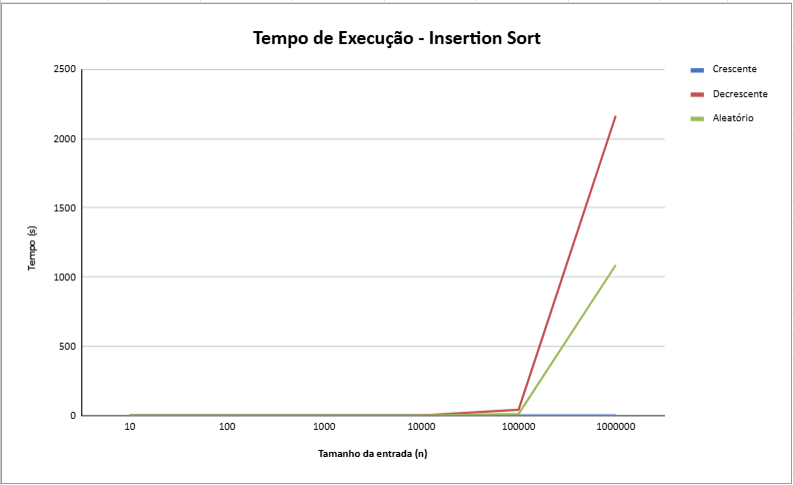
\includegraphics[width=0.85\textwidth]{Imagens/Insertion Sort/grafico insertion.png}
    \caption{Curvas de desempenho do Insertion Sort em função da ordenação e do tamanho da entrada ($n$).}
    \label{fig:insertion_grafico}
\end{figure}

\qquad A interpretação dos dados experimentais evidencia os seguintes padrões operacionais:

\begin{itemize}
    \item \textbf{Cenário Crescente (Melhor Caso):} O tempo de execução permaneceu inexpressivo até a escala de $1.000.000$ elementos (0,005 s), comprovando a eficiência do comportamento linear $O(n)$, decorrente da ausência de trocas internas no vetor.
    \item \textbf{Cenário Decrescente (Pior Caso):} Demonstra a inflexão característica da complexidade quadrática $O(n^2)$. O tempo eleva-se de 40,59 s ($n = 100.000$) para 2164,84 s ($\approx 36$ minutos para $n = 1.000.000$), consequência do custo máximo de comparações e deslocamentos a cada inserção.
    \item \textbf{Cenário Aleatório (Caso Médio):} O tempo registrado para $n = 1.000.000$ (1086,29 s) é aproximadamente metade do valor medido no pior caso. Esse resultado valida empiricamente o modelo matemático de constantes operacionais $T(n) \approx \frac{1}{2} T_{pior}(n)$, preservando a assíntota $O(n^2)$.
\end{itemize}
		\newpage
            \subsection{Bubble Sort}
		% --- Conteúdo ATUALIZADO para Tabela&Grafico/bubble_sort.tex ---

\qquad A seguir são apresentados os resultados obtidos na execução do algoritmo \textit{Bubble Sort}.

% --- IMAGEM DA TABELA DO BUBBLE SORT ---
\begin{figure}[h!]
    \centering
    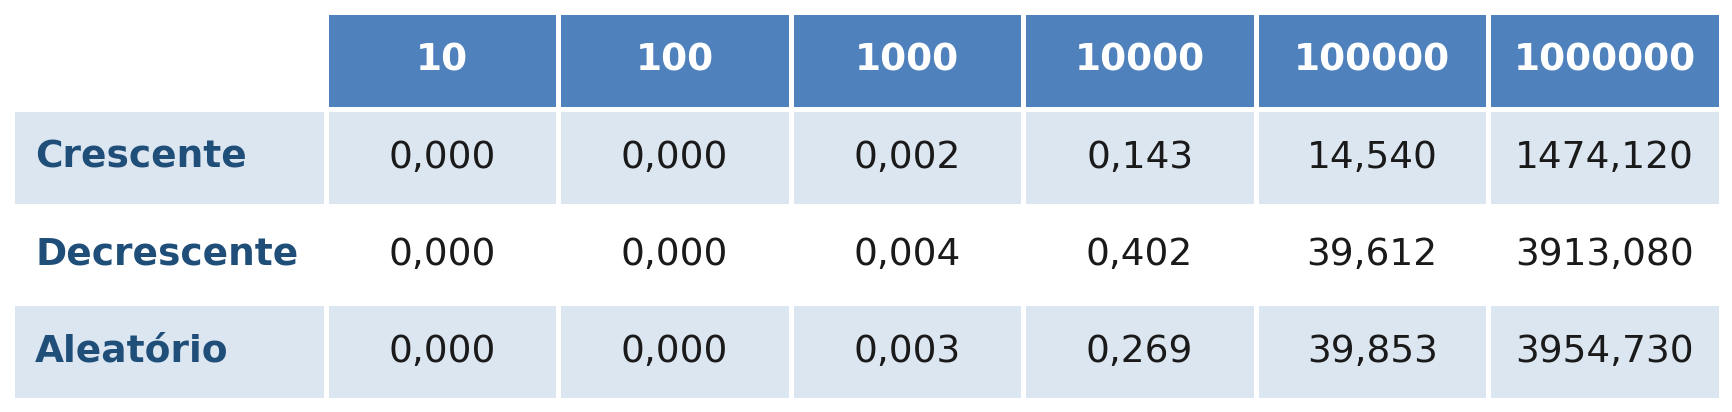
\includegraphics[width=1.0\textwidth]{Imagens/Bubble Sort/tabela_bubble.png}
    \caption{Tabela de tempo de execução (em segundos) do \textit{Bubble Sort} (elaborado pelo autor).}
    \label{fig:tabela_bubble}
\end{figure}

% --- IMAGEM DO GRÁFICO DO BUBBLE SORT ---
\begin{figure}[h!]
    \centering
    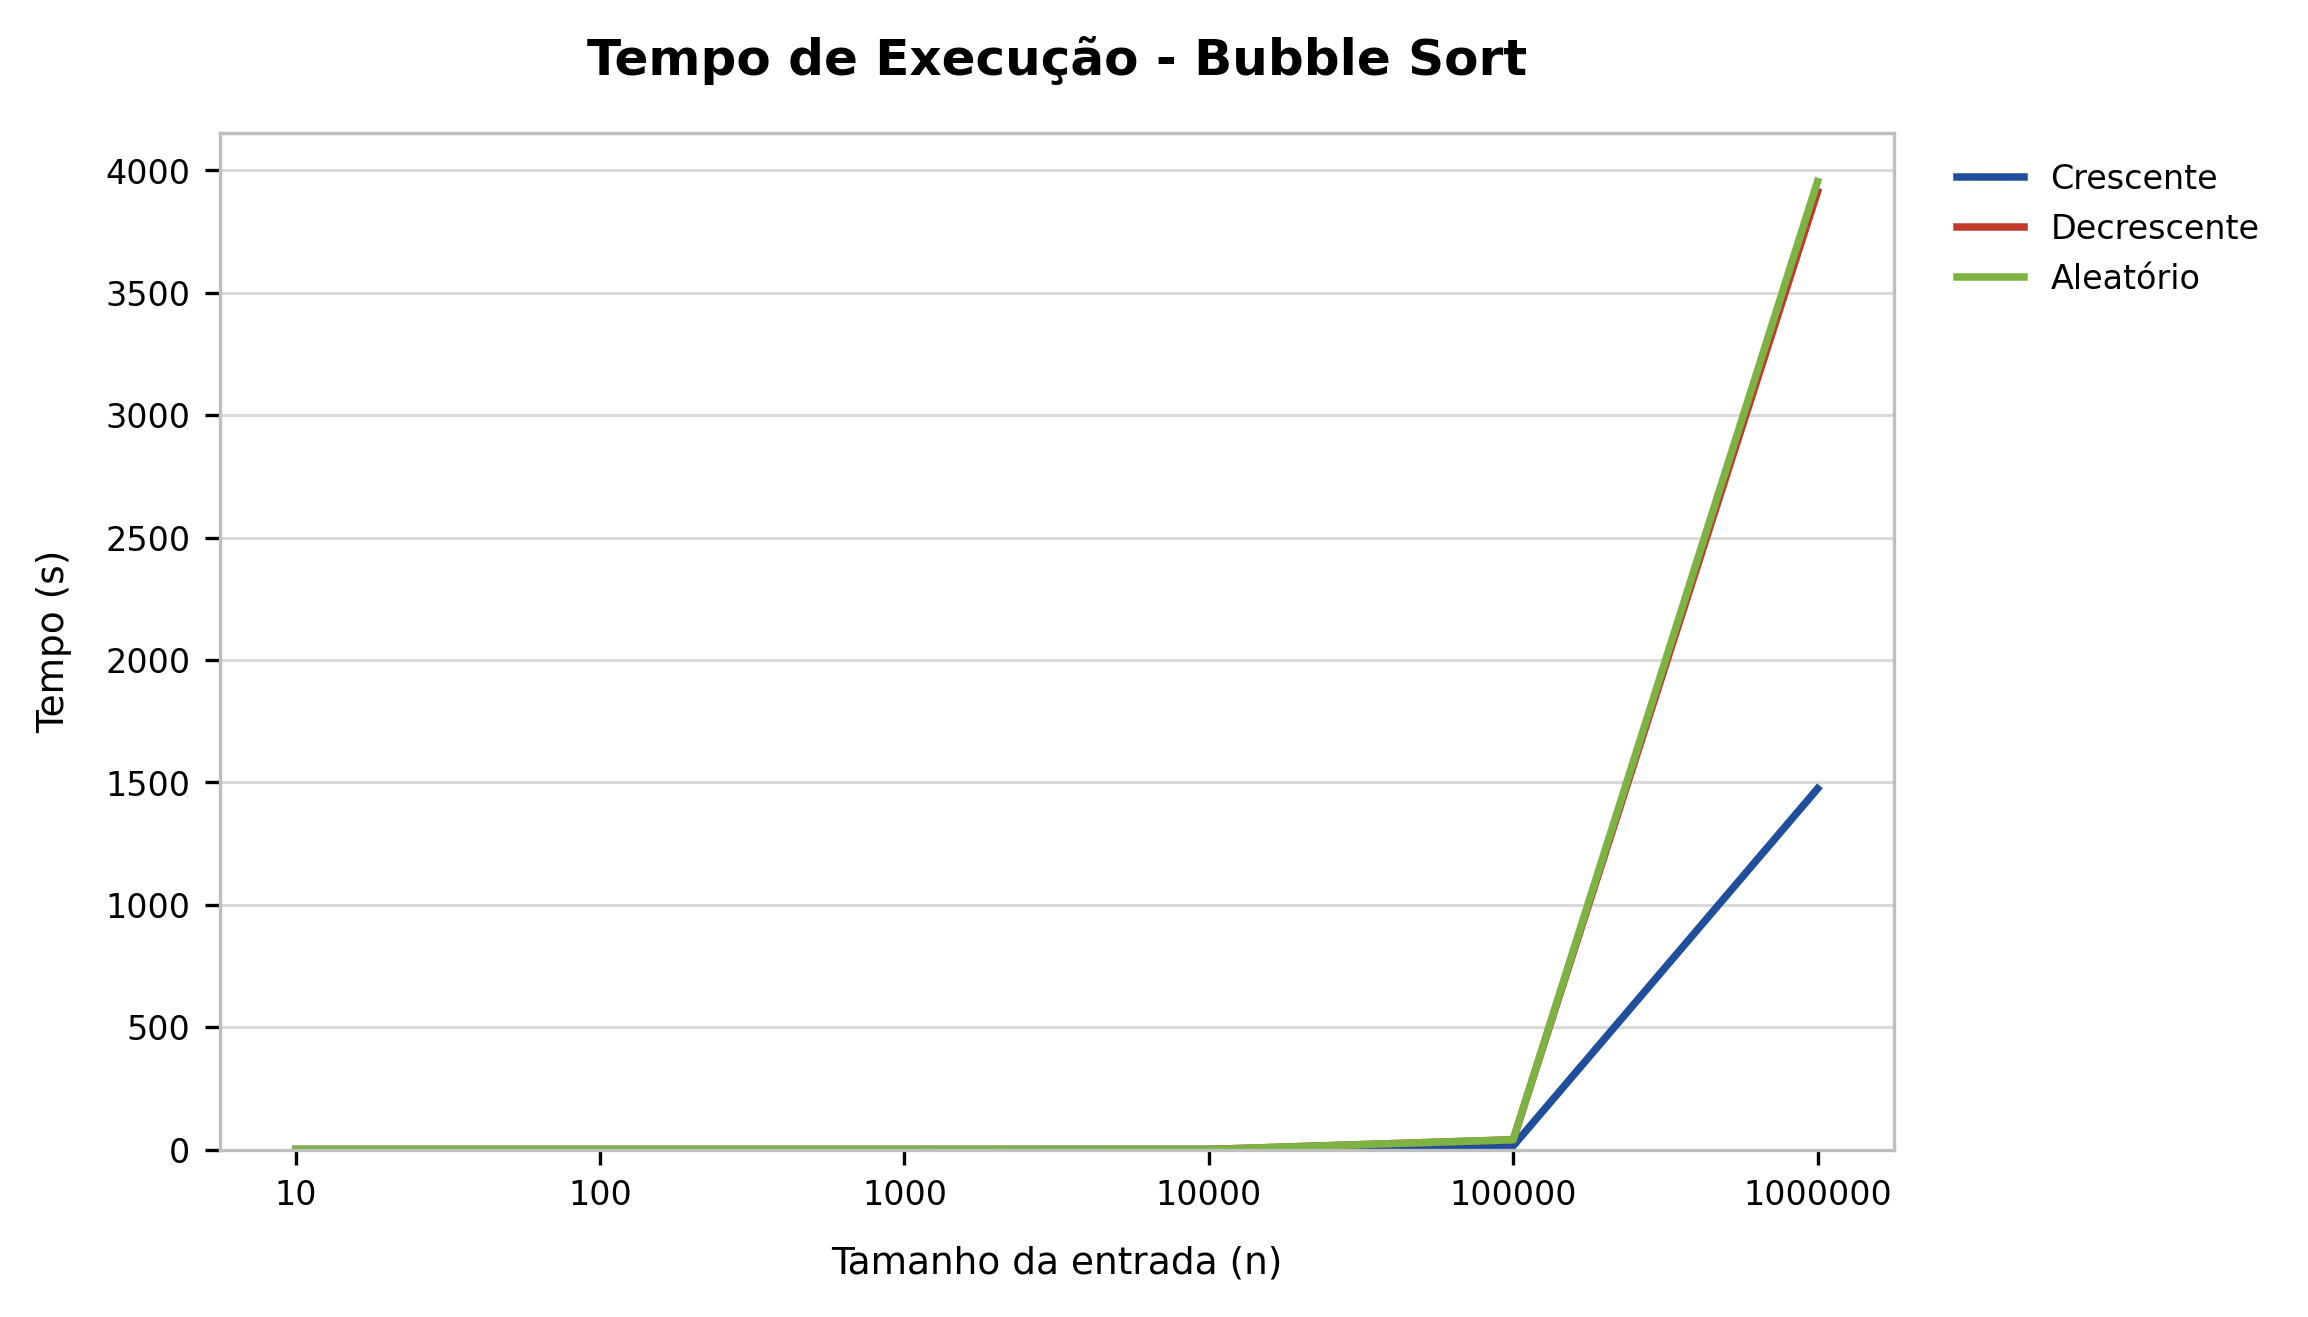
\includegraphics[width=1.0\textwidth]{Imagens/Bubble Sort/grafico_bubble.png}
    \caption{Desempenho do Algoritmo \textit{Bubble Sort} (elaborado pelo autor).}
    \label{fig:grafico_bubble}
\end{figure}

% --- ANÁLISE DOS RESULTADOS DO BUBBLE SORT ---

\qquad Os dados da Figura \ref{fig:tabela_bubble} e o gráfico da Figura \ref{fig:grafico_bubble} mostram o comportamento quadrático esperado para o \textit{Bubble Sort}, com tempos que se tornam proibitivos em entradas grandes. Para as entradas de 10 e 100 elementos, os tempos registrados foram de 0,000 segundo em todos os cenários, o que indica apenas que a duração ficou abaixo da precisão do relógio utilizado.

\begin{itemize}
    \item \textbf{Crescente (melhor caso):} mesmo com o vetor já ordenado, a implementação utilizada não possui mecanismo de parada antecipada, de modo que os laços aninhados são percorridos por completo. O tempo para um milhão de elementos foi de 1.474,120 segundos (cerca de 25 minutos). A vantagem desse cenário vem apenas da ausência de trocas, já que o número de comparações é o mesmo dos demais casos.

    \item \textbf{Decrescente (pior caso):} é o cenário que exige o número máximo de trocas, uma para cada comparação realizada. O tempo para um milhão de elementos foi de 3.913,080 segundos (aproximadamente 1 hora e 5 minutos), cerca de 2,7 vezes maior que o do vetor crescente.

    \item \textbf{Aleatório (caso médio):} o tempo foi de 3.954,730 segundos (aproximadamente 1 hora e 6 minutos), praticamente igual ao do pior caso. Isso mostra que, na prática, o \textit{Bubble Sort} não obtém ganho relevante em entradas desordenadas.
\end{itemize}

\qquad Um resultado que merece atenção é o fato de o caso aleatório ter sido ligeiramente mais lento que o decrescente, tanto em $n = 100.000$ (39,853 s contra 39,612 s) quanto em $n = 1.000.000$ (3.954,730 s contra 3.913,080 s), contrariando à primeira vista a expectativa teórica. A explicação está na implementação utilizada: como não há parada antecipada, o número de comparações é idêntico nos três cenários, e apenas o número de trocas varia. No vetor decrescente todas as comparações resultam em troca, mas seguindo um padrão regular de acesso à memória; no vetor aleatório o padrão é irregular, o que aumenta os erros de previsão de desvio no processador. A diferença observada, inferior a 1\%, está dentro da variação esperada para medições em hardware real e não altera a classificação de complexidade.

\qquad De modo geral, os testes confirmam o comportamento $O(n^2)$ do \textit{Bubble Sort} em todos os cenários avaliados para a implementação utilizada, o que o torna inadequado para conjuntos de dados de grande porte.

\FloatBarrier
		\newpage
            \subsection{Selection Sort}
		% --- Conteúdo ATUALIZADO para Tabela&Grafico/selection_sort.tex ---

\qquad A seguir são apresentados os resultados obtidos na execução do algoritmo \textit{Selection Sort}.

% --- IMAGEM DA TABELA DO SELECTION SORT ---
\begin{figure}[h!]
    \centering
    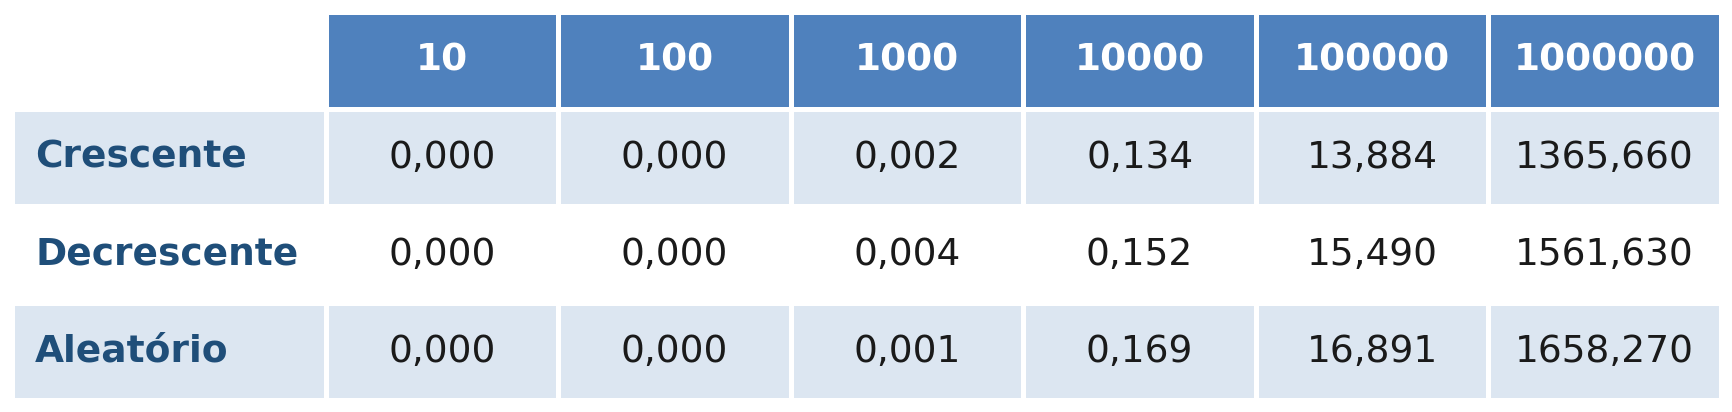
\includegraphics[width=1.0\textwidth]{Imagens/Selection Sort/tabela_selection.png}
    \caption{Tabela de tempo de execução (em segundos) do \textit{Selection Sort} (elaborado pelo autor).}
    \label{fig:tabela_selection}
\end{figure}

% --- IMAGEM DO GRÁFICO DO SELECTION SORT ---
\begin{figure}[h!]
    \centering
    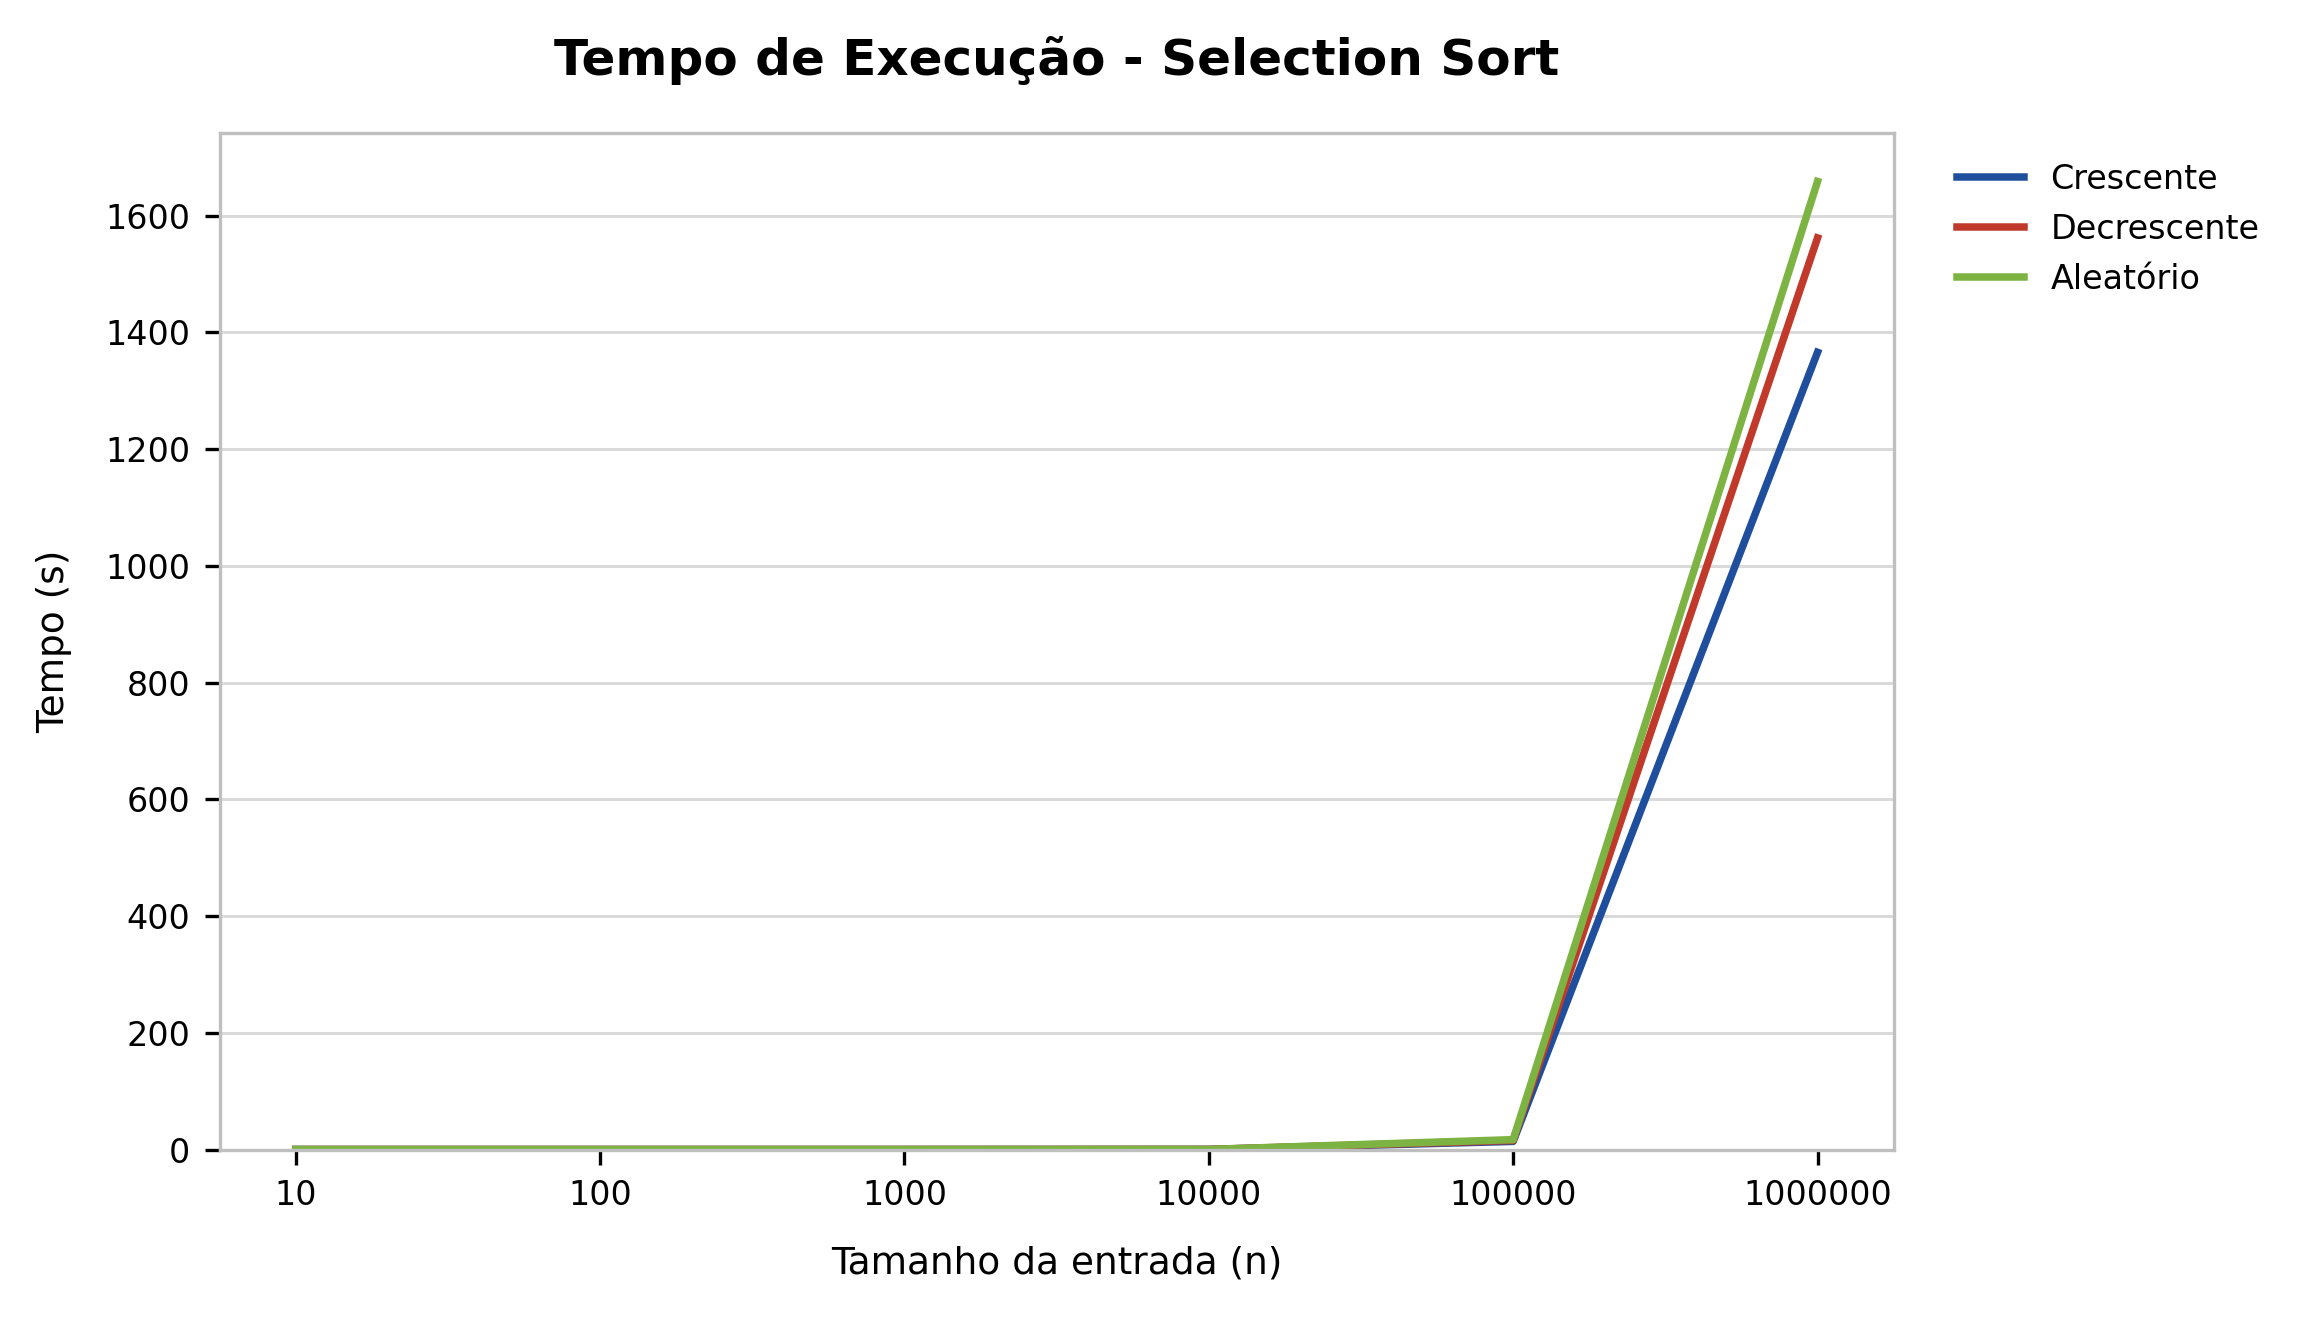
\includegraphics[width=1.0\textwidth]{Imagens/Selection Sort/grafico_selection.png}
    \caption{Desempenho do Algoritmo \textit{Selection Sort} (elaborado pelo autor).}
    \label{fig:grafico_selection}
\end{figure}

% --- ANÁLISE DOS RESULTADOS DO SELECTION SORT ---

\qquad Os dados da Figura \ref{fig:tabela_selection} e o gráfico da Figura \ref{fig:grafico_selection} evidenciam a principal característica do \textit{Selection Sort}: a pouca sensibilidade à ordem inicial dos dados. Para as entradas de 10 e 100 elementos, os tempos registrados foram de 0,000 segundo em todos os cenários, o que indica apenas que a duração ficou abaixo da precisão do relógio utilizado.

\begin{itemize}
    \item \textbf{Desempenho consistente entre os cenários:} os tempos para um milhão de elementos foram de 1.365,660 segundos (crescente), 1.561,630 segundos (decrescente) e 1.658,270 segundos (aleatório), todos entre 22 e 28 minutos. A diferença entre o menor e o maior tempo é de aproximadamente 21\%, valor pequeno quando comparado à diferença de mais de 160\% observada no \textit{Bubble Sort} entre o melhor e o pior cenário.

    \item \textbf{Origem dessa estabilidade:} o algoritmo executa sempre o mesmo número de comparações, $\frac{n(n-1)}{2}$, independentemente da ordem inicial do vetor, pois o laço interno precisa percorrer toda a porção não ordenada para localizar o menor elemento. O número de trocas também é fixo em $n-1$. A pequena variação observada entre os cenários vem apenas das atualizações do índice \texttt{min\_idx}, que ocorrem com frequências diferentes conforme a distribuição dos dados.

    \item \textbf{Complexidade quadrática:} o crescimento dos tempos acompanha o esperado para $O(n^2)$. Ao passar de 100.000 para 1.000.000 de elementos, entrada dez vezes maior, o tempo do caso aleatório passou de 16,891 s para 1.658,270 s, um aumento de aproximadamente 98 vezes, valor bastante próximo das 100 vezes previstas pela análise teórica.
\end{itemize}

\qquad Comparado ao \textit{Bubble Sort}, o \textit{Selection Sort} apresentou desempenho superior em todos os cenários com um milhão de elementos, especialmente nas entradas decrescente e aleatória, onde foi cerca de 2,4 vezes mais rápido. Essa vantagem decorre do menor número de trocas realizadas: enquanto o \textit{Bubble Sort} pode efetuar uma troca a cada comparação, o \textit{Selection Sort} realiza no máximo $n-1$ trocas ao todo.

\qquad De modo geral, os testes mostram um algoritmo de desempenho estável e previsível, mas ainda assim inadequado para entradas grandes, já que não obtém qualquer vantagem quando os dados estão parcialmente ordenados.

\FloatBarrier
		\newpage
            \subsection{Shell Sort}
		% --- Conteúdo ATUALIZADO para Tabela&Grafico/shell_sort.tex ---

\qquad A seguir são apresentados os resultados obtidos na execução do algoritmo \textit{Shell Sort}.

% --- IMAGEM DA TABELA DO SHELL SORT ---
\begin{figure}[h!]
    \centering
    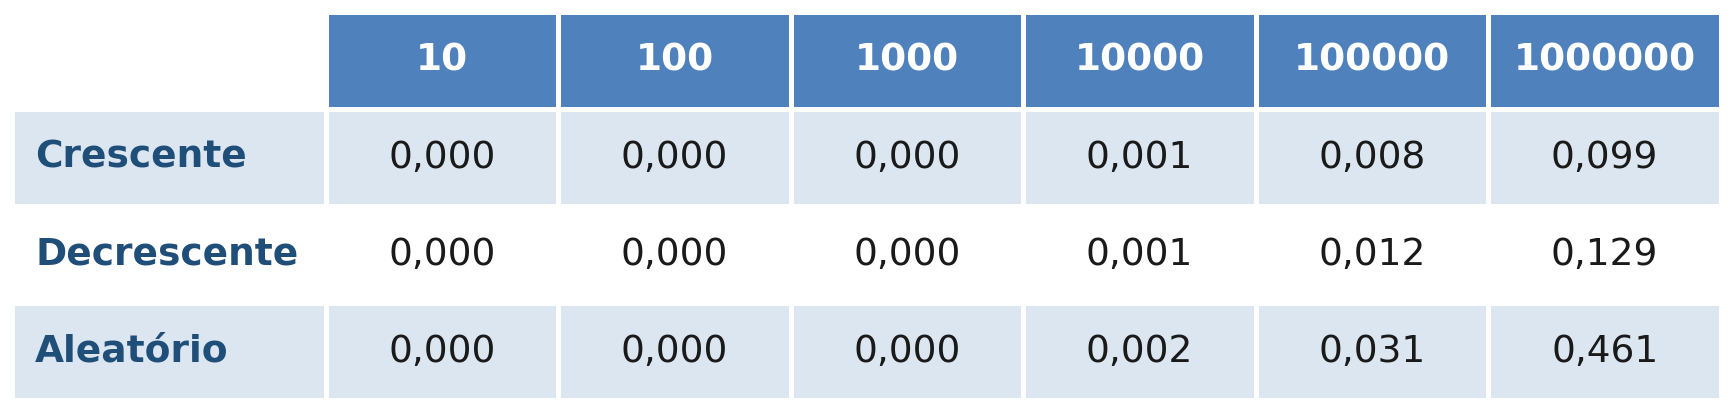
\includegraphics[width=1.0\textwidth]{Imagens/Shell_sort/tabela_shell.png}
    \caption{Tabela de tempo de execução (em segundos) do \textit{Shell Sort} (elaborado pelo autor).}
    \label{fig:tabela_shell}
\end{figure}

% --- IMAGEM DO GRÁFICO DO SHELL SORT ---
\begin{figure}[h!]
    \centering
    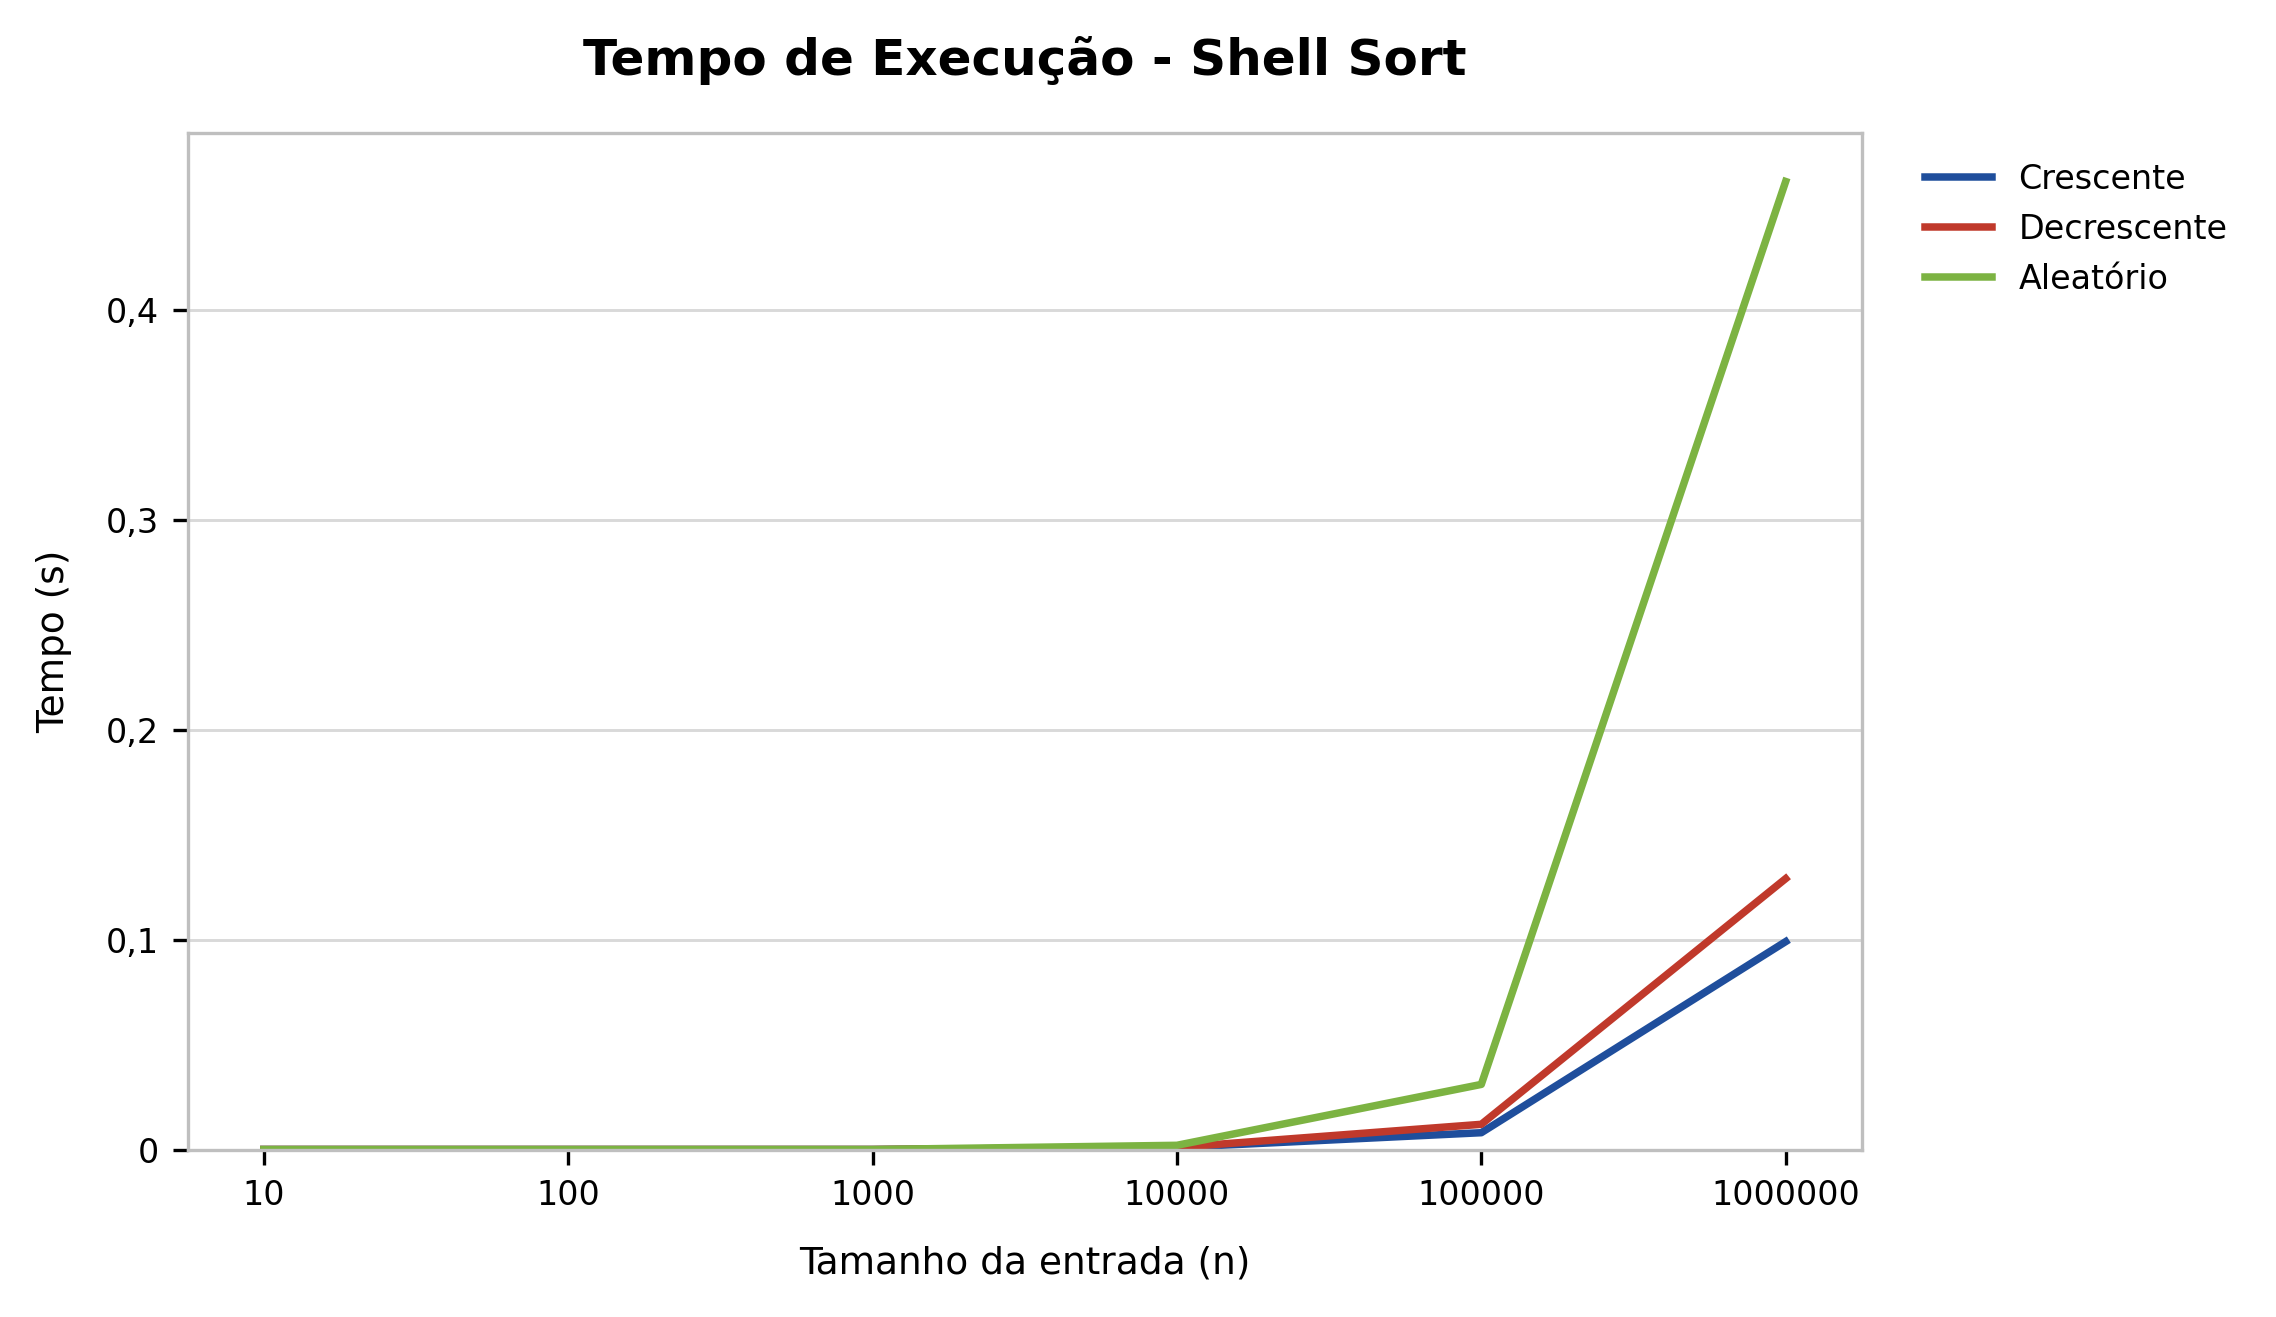
\includegraphics[width=1.0\textwidth]{Imagens/Shell_sort/grafico_shell.png}
    \caption{Desempenho do Algoritmo \textit{Shell Sort} (elaborado pelo autor).}
    \label{fig:grafico_shell}
\end{figure}

% --- ANÁLISE DOS RESULTADOS DO SHELL SORT ---

\qquad Os dados da Figura \ref{fig:tabela_shell} e o gráfico da Figura \ref{fig:grafico_shell} mostram uma diferença expressiva de desempenho em relação aos algoritmos quadráticos analisados anteriormente. Para as entradas de 10, 100 e 1.000 elementos, os tempos registrados foram de 0,000 segundo em todos os cenários, o que indica apenas que a duração ficou abaixo da precisão do relógio utilizado. Diferenças só passam a ser perceptíveis a partir de 10.000 elementos.

\begin{itemize}
    \item \textbf{Desempenho subquadrático:} para ordenar um milhão de elementos no cenário aleatório, o \textit{Shell Sort} levou 0,461 segundo, enquanto o \textit{Selection Sort} levou 1.658,270 segundos e o \textit{Bubble Sort}, 3.954,730 segundos. Isso representa um desempenho cerca de 3.600 e 8.600 vezes superior, respectivamente.

    \item \textbf{Crescimento dos tempos:} ao passar de 100.000 para 1.000.000 de elementos, entrada dez vezes maior, o tempo do caso aleatório passou de 0,031 s para 0,461 s, um crescimento de aproximadamente 15 vezes. Em um algoritmo quadrático, o mesmo aumento resultaria em um tempo cerca de 100 vezes maior, como de fato ocorreu com o \textit{Selection Sort}. Esse resultado é compatível com a complexidade esperada para a sequência de \textit{gaps} utilizada.

    \item \textbf{Influência da ordem inicial:} a ordem dos dados ainda afeta o desempenho, mas de forma muito menos acentuada. O vetor crescente foi o mais rápido (0,099 s), seguido pelo decrescente (0,129 s) e pelo aleatório (0,461 s). O cenário aleatório é o mais custoso porque os elementos precisam percorrer distâncias maiores até suas posições finais, enquanto nas entradas ordenada e invertida a estrutura regular dos dados permite deslocamentos mais previsíveis.
\end{itemize}

\qquad Os resultados mostram que o \textit{Shell Sort} é consideravelmente mais eficiente que os métodos quadráticos simples, mantendo tempos inferiores a um segundo mesmo para um milhão de elementos, o que o torna uma alternativa viável para conjuntos de dados de tamanho médio a grande.

\FloatBarrier
		\newpage
            \subsection{Merge Sort}
		\qquad A seguir são apresentados os resultados obtidos na execução do algoritmo \textit{Merge Sort}.

% --- IMAGEM DA TABELA DO MERGE SORT ---
\begin{figure}[h!]
    \centering
    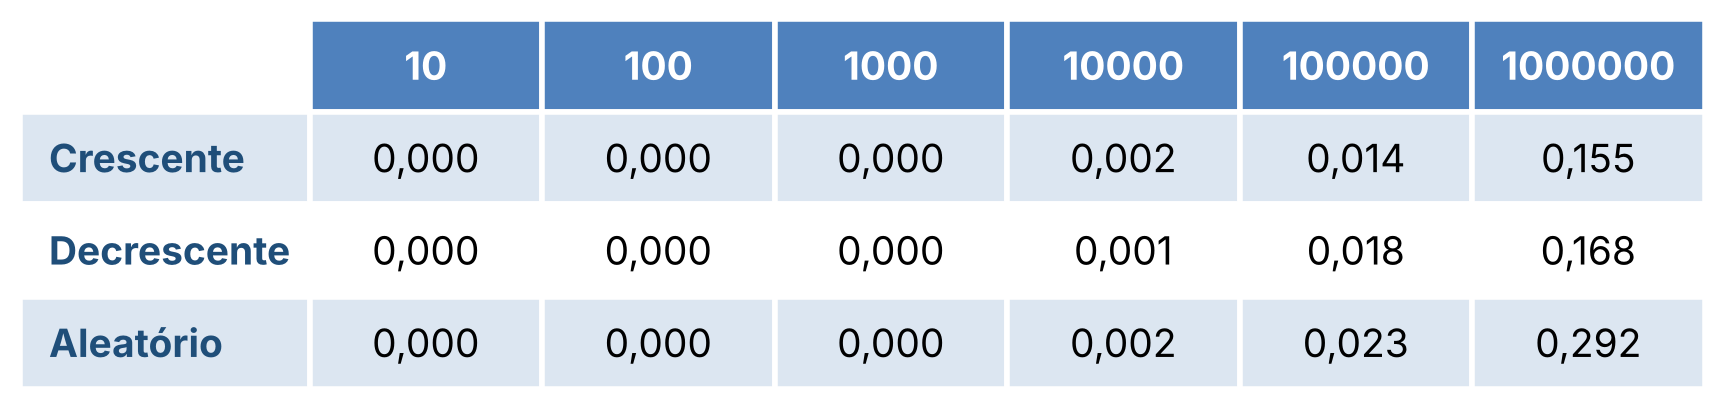
\includegraphics[width=1.0\textwidth]{Imagens/Merge Sort/tabela_merge.png}
    \caption{Tabela de tempo de execução (em segundos) do \textit{Merge Sort} (elaborado pelo autor).}
    \label{fig:tabela_merge}
\end{figure}

% --- IMAGEM DO GRÁFICO DO MERGE SORT ---
\begin{figure}[h!]
    \centering
    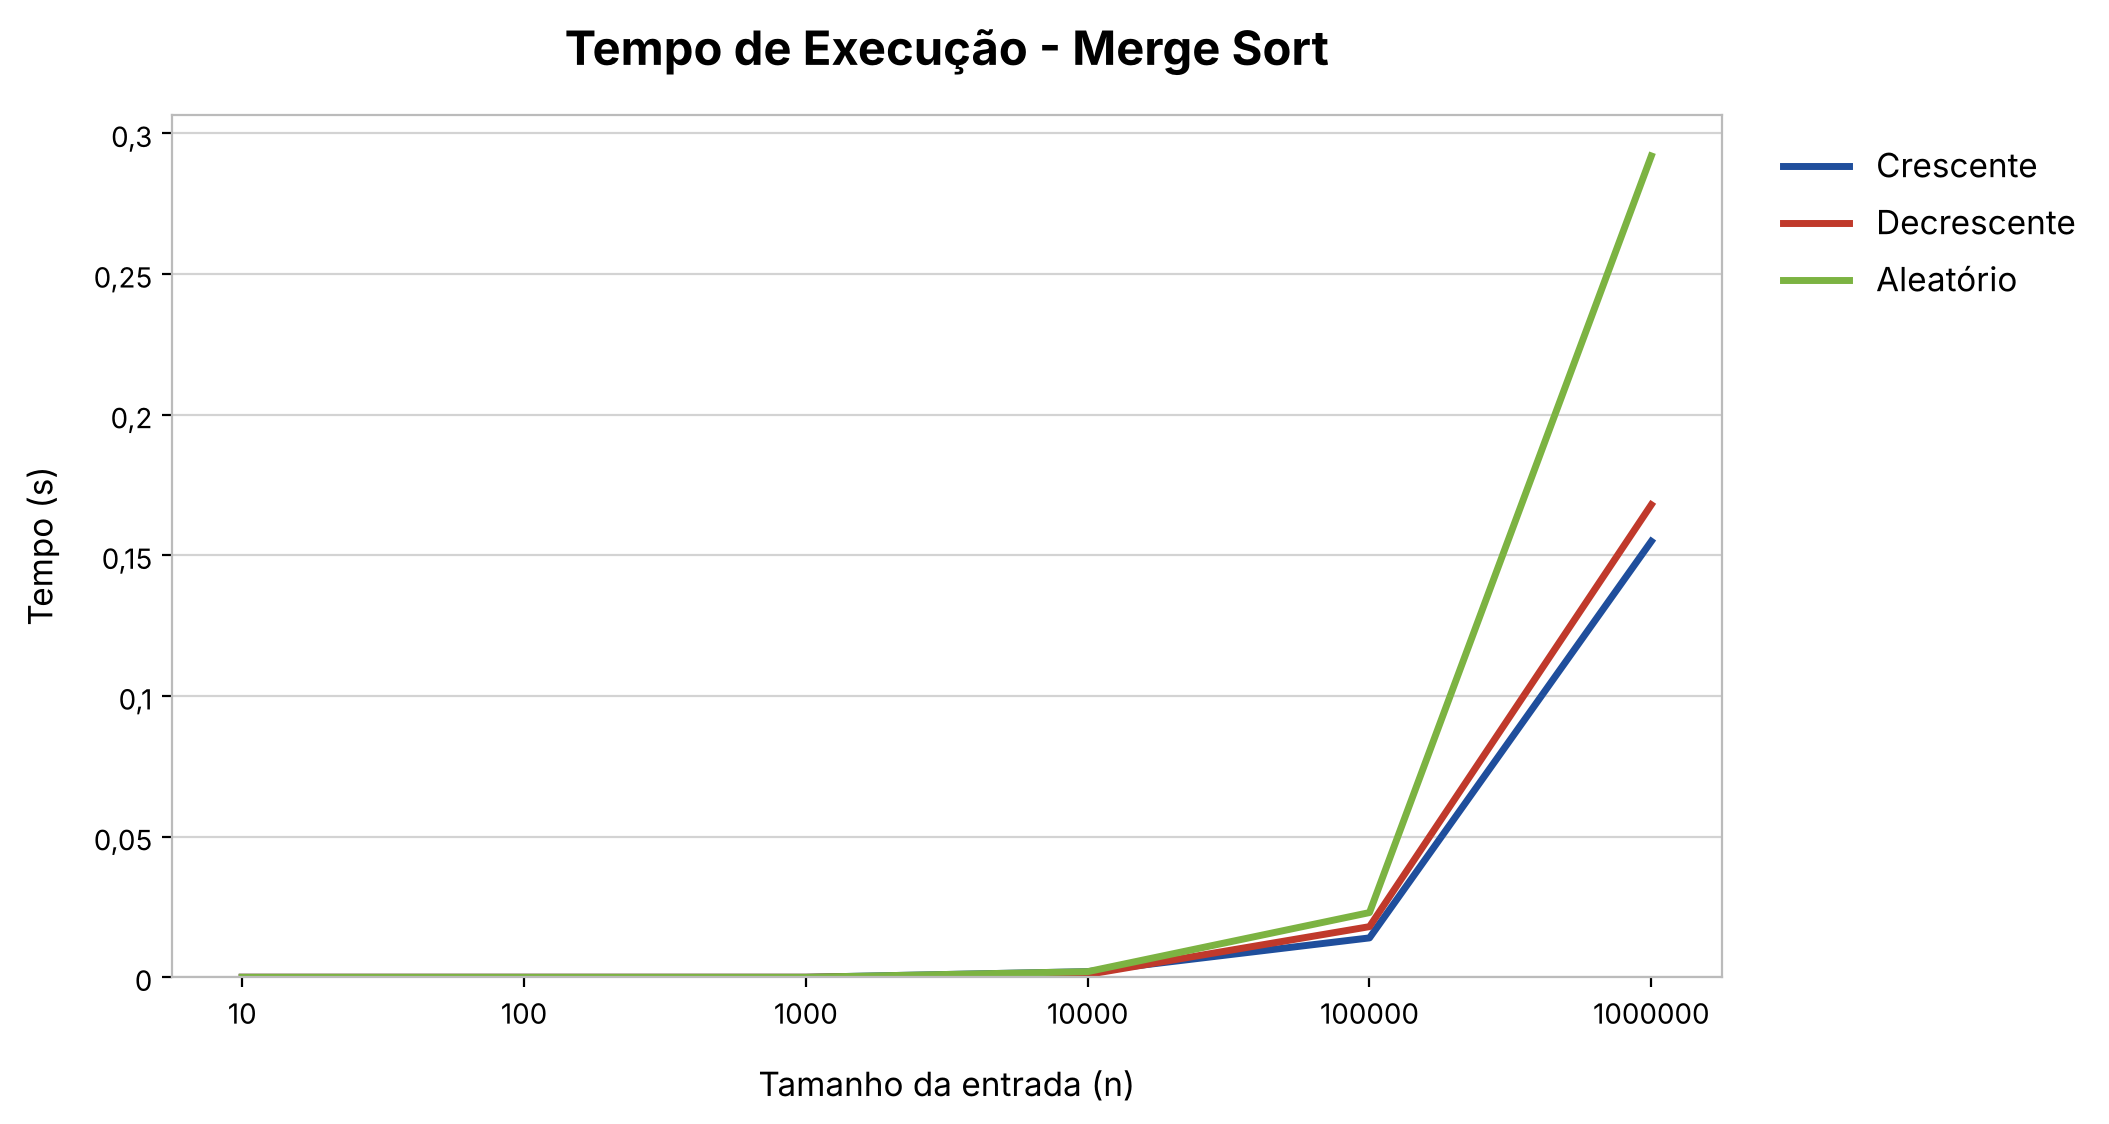
\includegraphics[width=1.0\textwidth]{Imagens/Merge Sort/grafico_merge.png}
    \caption{Desempenho do Algoritmo \textit{Merge Sort} (elaborado pelo autor).}
    \label{fig:grafico_merge}
\end{figure}

% --- ANÁLISE DOS RESULTADOS DO MERGE SORT ---

\qquad Os dados da Figura \ref{fig:tabela_merge} e o gráfico da Figura \ref{fig:grafico_merge} mostram que o \textit{Merge Sort} manteve tempos muito baixos em todos os cenários. Para as entradas de 10, 100 e 1.000 elementos, os tempos registrados foram de 0,000 segundo, o que indica apenas que a duração ficou abaixo da precisão do relógio utilizado. Diferenças só passam a ser perceptíveis a partir de 10.000 elementos.

\begin{itemize}
    \item \textbf{Desempenho em relação aos algoritmos quadráticos:} para ordenar um milhão de elementos no cenário aleatório, o \textit{Merge Sort} levou 0,292 segundo, enquanto o \textit{Selection Sort} levou 1.658,270 segundos e o \textit{Bubble Sort}, 3.954,730 segundos. Isso representa um desempenho cerca de 5.700 e 13.500 vezes superior, respectivamente.

    \item \textbf{Crescimento dos tempos:} ao passar de 100.000 para 1.000.000 de elementos, entrada dez vezes maior, o tempo do caso aleatório passou de 0,023 s para 0,292 s, um crescimento de aproximadamente 12,7 vezes. Esse valor é próximo do esperado para $n \log n$, que é de cerca de 12 vezes, e muito inferior às 100 vezes esperadas para um algoritmo quadrático. Os cenários crescente e decrescente cresceram cerca de 11 e 9 vezes, respectivamente.

    \item \textbf{Influência da ordem inicial:} diferente dos algoritmos quadráticos, a ordem dos dados teve pouco efeito sobre o desempenho. Para um milhão de elementos, os tempos foram de 0,155 s (crescente), 0,168 s (decrescente) e 0,292 s (aleatório). Isso é coerente com a análise teórica, segundo a qual o algoritmo realiza o mesmo número de divisões e intercalações em qualquer ordem. O cenário aleatório foi o mais lento, o que provavelmente se deve ao comportamento do processador, pois em entradas ordenadas as comparações da intercalação seguem um padrão previsível.
\end{itemize}

\qquad Em comparação com o \textit{Shell Sort}, o \textit{Merge Sort} foi mais rápido no cenário aleatório (0,292 s contra 0,461 s para um milhão de elementos), mas foi mais lento nos cenários crescente (0,155 s contra 0,099 s) e decrescente (0,168 s contra 0,129 s). Isso acontece porque o \textit{Shell Sort} aproveita a ordenação prévia dos dados, enquanto o \textit{Merge Sort} sempre executa todas as divisões e intercalações e ainda copia os elementos para o vetor auxiliar.

\qquad Os resultados mostram que o \textit{Merge Sort} é o algoritmo mais regular entre os estudados, com desempenho previsível e tempos inferiores a meio segundo para um milhão de elementos. Em contrapartida, ele exige memória adicional proporcional ao tamanho da entrada, o que o diferencia dos demais algoritmos deste trabalho.

\FloatBarrier
		\newpage
            \subsection{Comparativo Geral}
		% --- Conteúdo FINAL para Tabela&Grafico/comparativo_geral.tex ---

\qquad A etapa final do trabalho consiste na análise comparativa do desempenho dos cinco algoritmos estudados: \textit{Bubble Sort}, \textit{Insertion Sort}, \textit{Selection Sort}, \textit{Shell Sort} e \textit{Merge Sort}. Para facilitar a interpretação, os resultados foram organizados por cenário de entrada, cada um com sua tabela de tempos e seu gráfico correspondente. Em todas as figuras, cada algoritmo é identificado por uma cor própria, mantida ao longo de toda a seção.

\qquad Os gráficos utilizam escala linear no eixo vertical, mantendo o mesmo padrão das figuras individuais de cada algoritmo. Como os tempos medidos variam de milésimos de segundo a mais de uma hora, as curvas dos algoritmos mais rápidos (\textit{Shell Sort} e \textit{Merge Sort}, além do \textit{Insertion Sort} no cenário crescente) aparecem rentes ao eixo horizontal. Isso não indica ausência de dados, e sim valores pequenos demais para serem distinguidos em uma escala que precisa acomodar milhares de segundos. Os valores exatos podem ser consultados nas tabelas que acompanham cada gráfico.

\qquad Os nomes dados aos cenários (melhor, pior e médio caso) se referem ao comportamento dos algoritmos quadráticos e do \textit{Shell Sort}, cujo desempenho depende da ordem inicial dos dados. No caso do \textit{Merge Sort}, esses nomes indicam apenas o tipo de entrada utilizada, pois o algoritmo executa o mesmo trabalho em qualquer ordem.

\subsubsection*{Análise Comparativa por Cenário}

\paragraph{Cenário Crescente (Melhor Caso)}
A Figura \ref{fig:tabela_comp_melhor} e a Figura \ref{fig:grafico_comp_melhor} mostram o desempenho dos algoritmos com um vetor já ordenado. É neste cenário que se observa a maior diferença entre eles. O \textbf{Insertion Sort} levou apenas 0,005 segundo para um milhão de elementos, resultado que reflete sua complexidade $O(n)$ no melhor caso: com o vetor ordenado, a condição do laço interno falha na primeira verificação e nenhum deslocamento é realizado. O \textbf{Shell Sort} levou 0,099 segundo, também beneficiado pela ordenação prévia. O \textbf{Merge Sort} levou 0,155 segundo: ele não tira proveito da ordenação, pois executa todas as divisões e intercalações mesmo com o vetor ordenado, mas seu custo $O(n \log n)$ já é baixo o bastante para ficar próximo dos dois anteriores. Em contraste, o \textbf{Bubble Sort} (1.474,120s) e o \textbf{Selection Sort} (1.365,660s) mantiveram comportamento quadrático, pois nenhuma das duas implementações possui mecanismo capaz de detectar que o vetor já está ordenado e interromper a execução.

\begin{figure}[!htb]
    \centering
    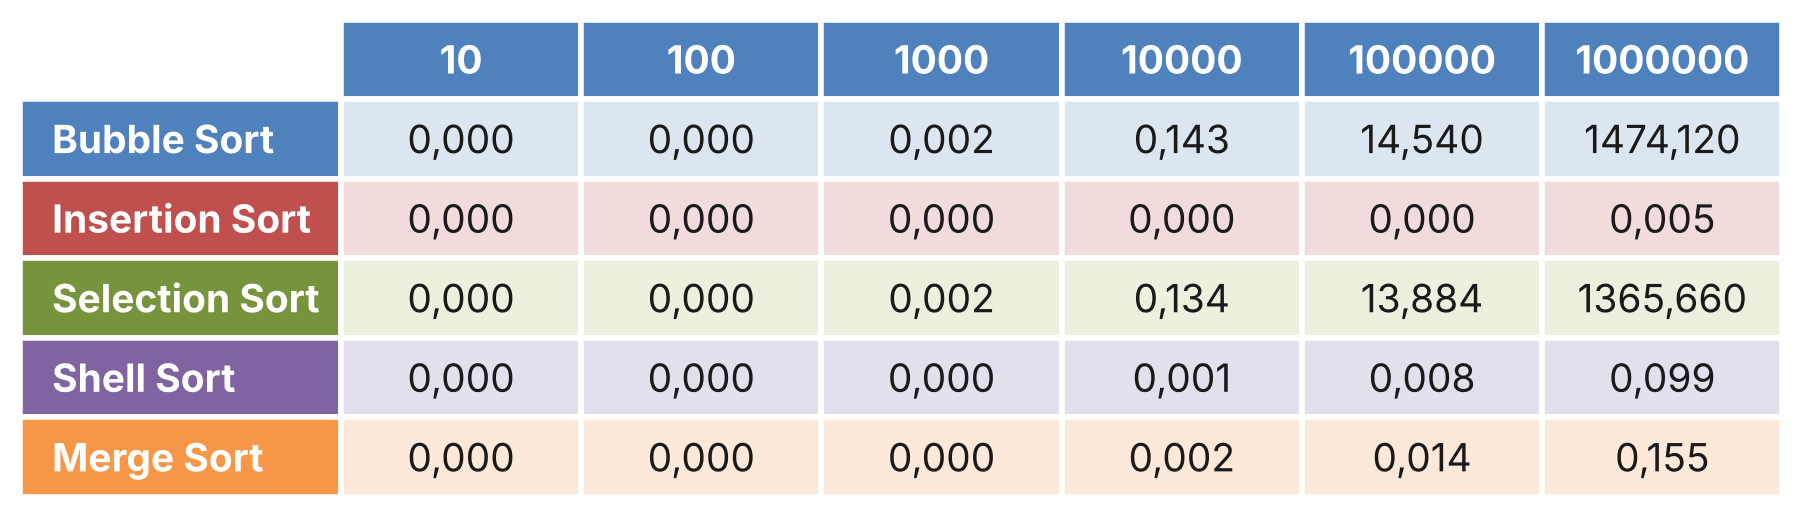
\includegraphics[width=0.8\textwidth]{Imagens/Geral/tabela_comp_melhorcaso.png}
    \caption{Tempos de execução (em segundos) dos cinco algoritmos - Cenário Crescente (elaborado pelo autor).}
    \label{fig:tabela_comp_melhor}

    \vspace{0.5cm}

    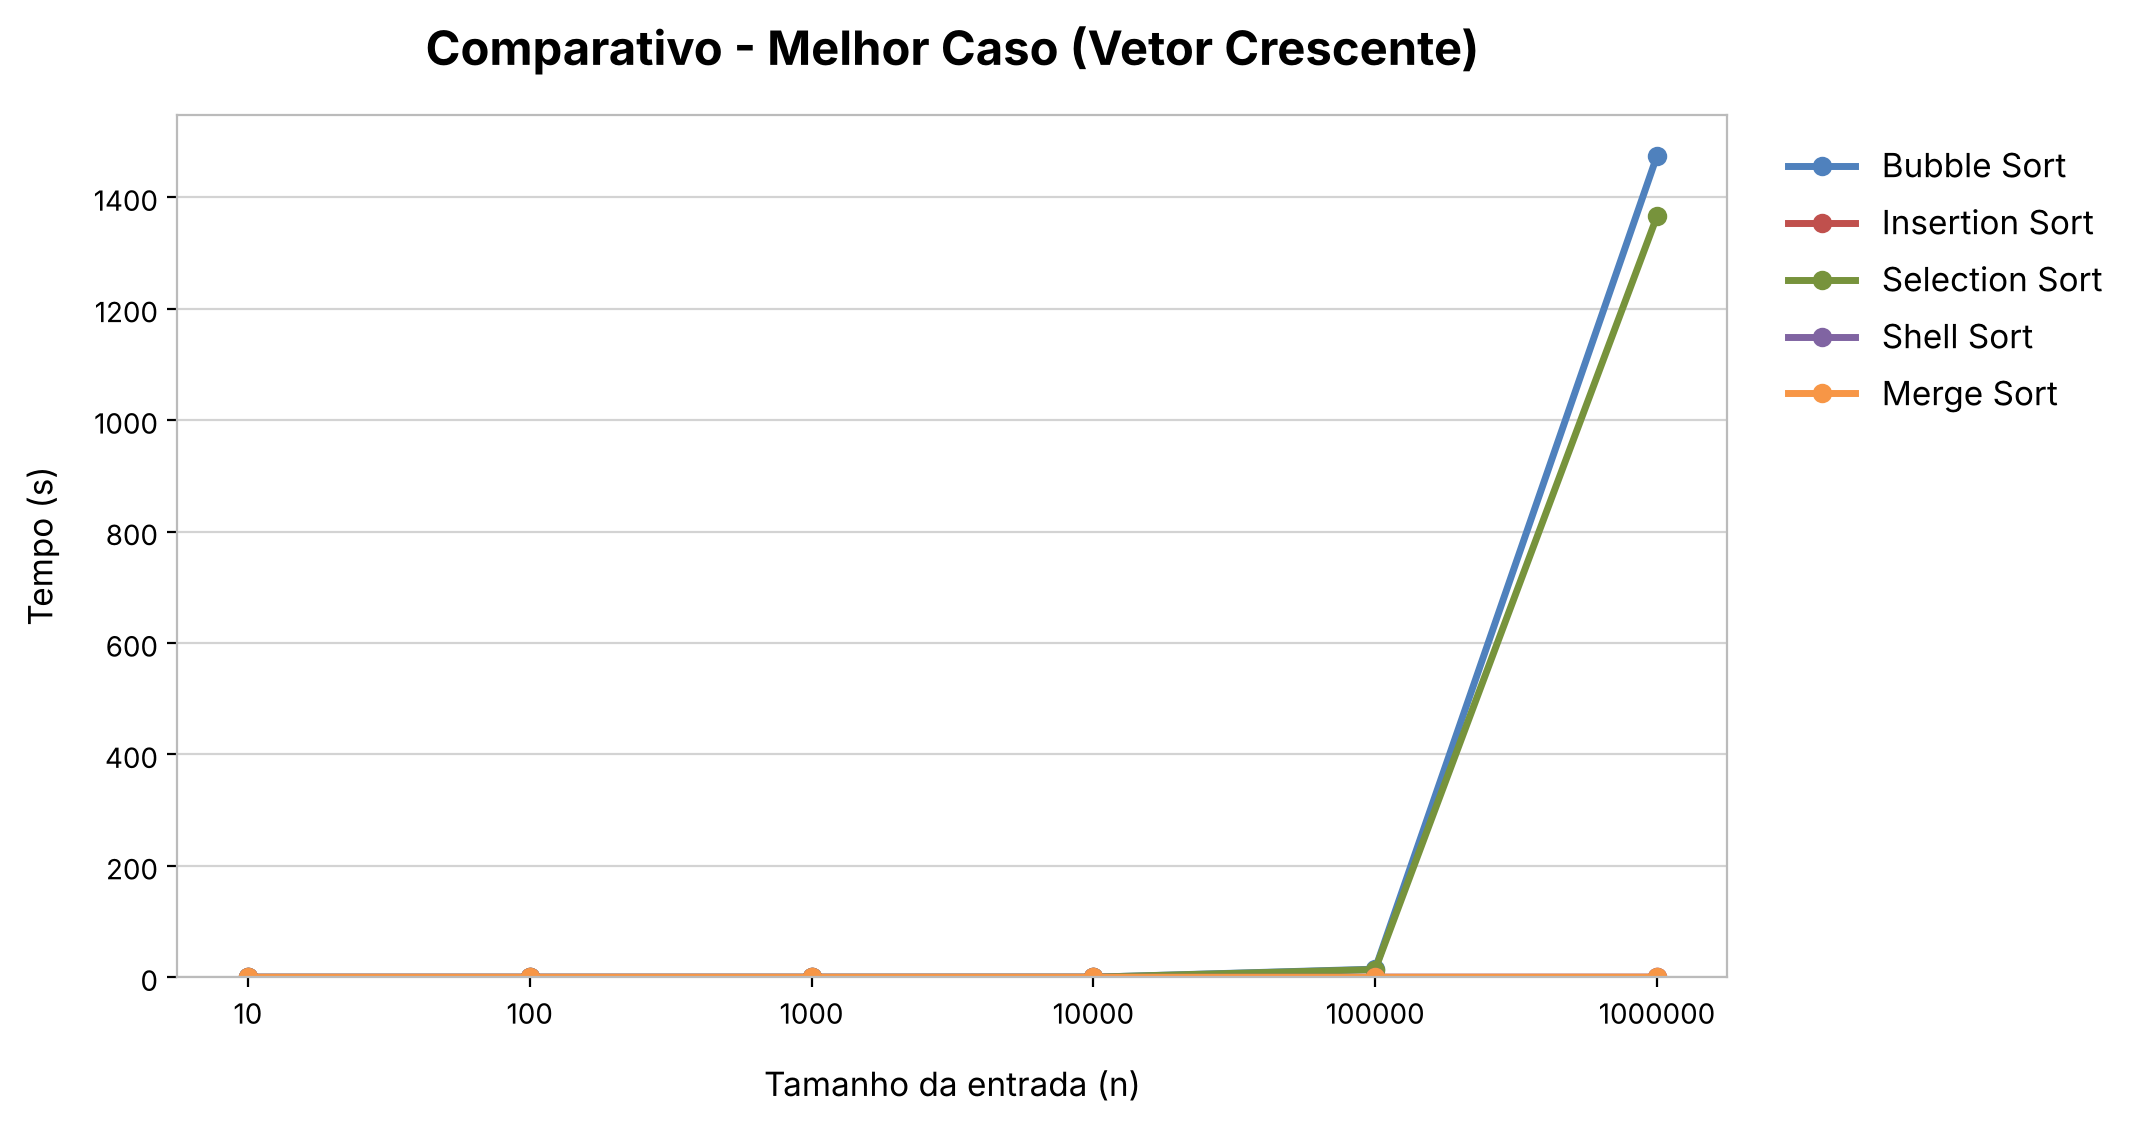
\includegraphics[width=0.8\textwidth]{Imagens/Geral/grafico_comp_melhorcaso.png}
    \caption{Comparativo de Desempenho dos Algoritmos - Cenário Crescente (elaborado pelo autor).}
    \label{fig:grafico_comp_melhor}
\end{figure}

\FloatBarrier

\paragraph{Cenário Decrescente (Pior Caso)}
Com os dados em ordem inversa, apresentados na Figura \ref{fig:tabela_comp_pior} e na Figura \ref{fig:grafico_comp_pior}, os algoritmos quadráticos são os mais exigidos. O \textbf{Shell Sort} (0,129 segundo) e o \textbf{Merge Sort} (0,168 segundo) permanecem ordens de grandeza mais rápidos, com tempos muito próximos entre si. O tempo do \textit{Merge Sort} neste cenário é praticamente o mesmo do cenário crescente (0,155s), o que confirma que seu desempenho não depende da ordem dos dados. Entre os quadráticos, o \textbf{Bubble Sort} apresenta o pior desempenho absoluto, com 3.913,080s (aproximadamente 1h05min), por realizar uma troca a cada comparação efetuada. O \textbf{Insertion Sort} (2.164,840s) e o \textbf{Selection Sort} (1.561,630s) também se mostram impraticáveis nesta escala, com vantagem para o \textit{Selection Sort}, que se limita a $n-1$ trocas no total, independentemente da ordem inicial dos dados.

\begin{figure}[!htb]
    \centering
    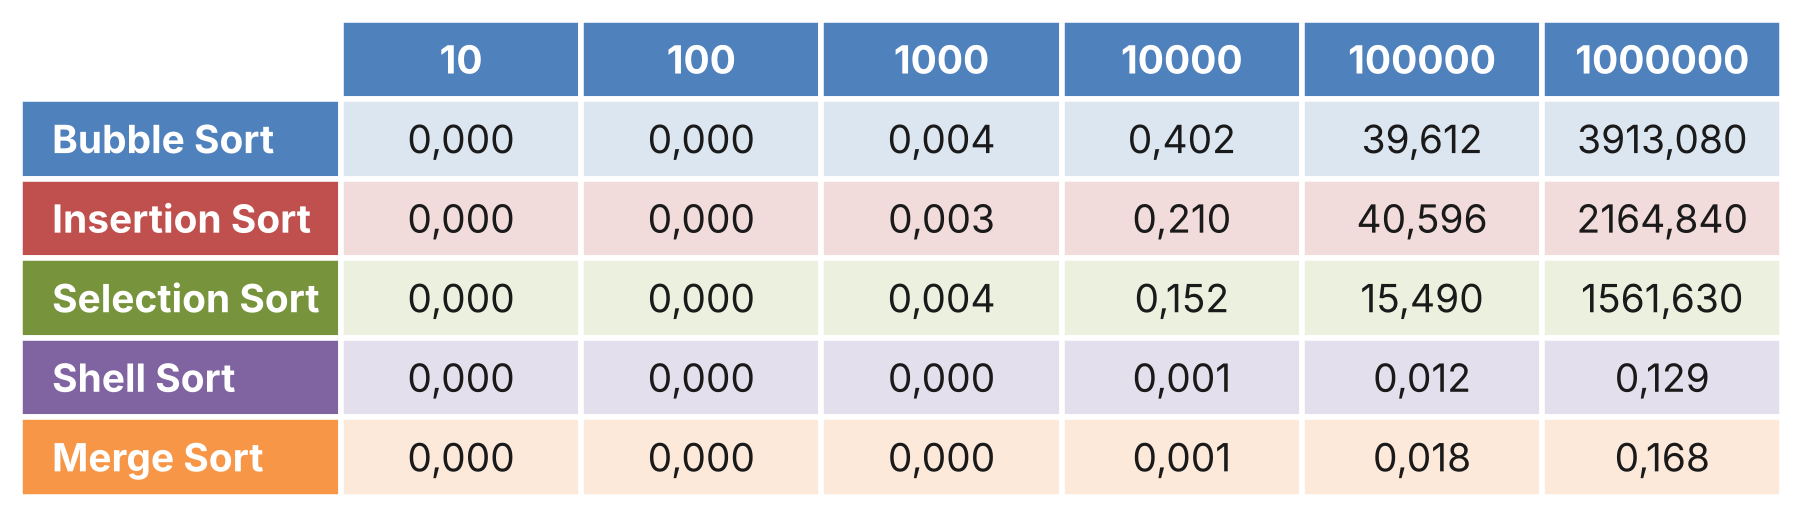
\includegraphics[width=0.8\textwidth]{Imagens/Geral/tabela_comp_piorcaso.png}
    \caption{Tempos de execução (em segundos) dos cinco algoritmos - Cenário Decrescente (elaborado pelo autor).}
    \label{fig:tabela_comp_pior}

    \vspace{0.5cm}

    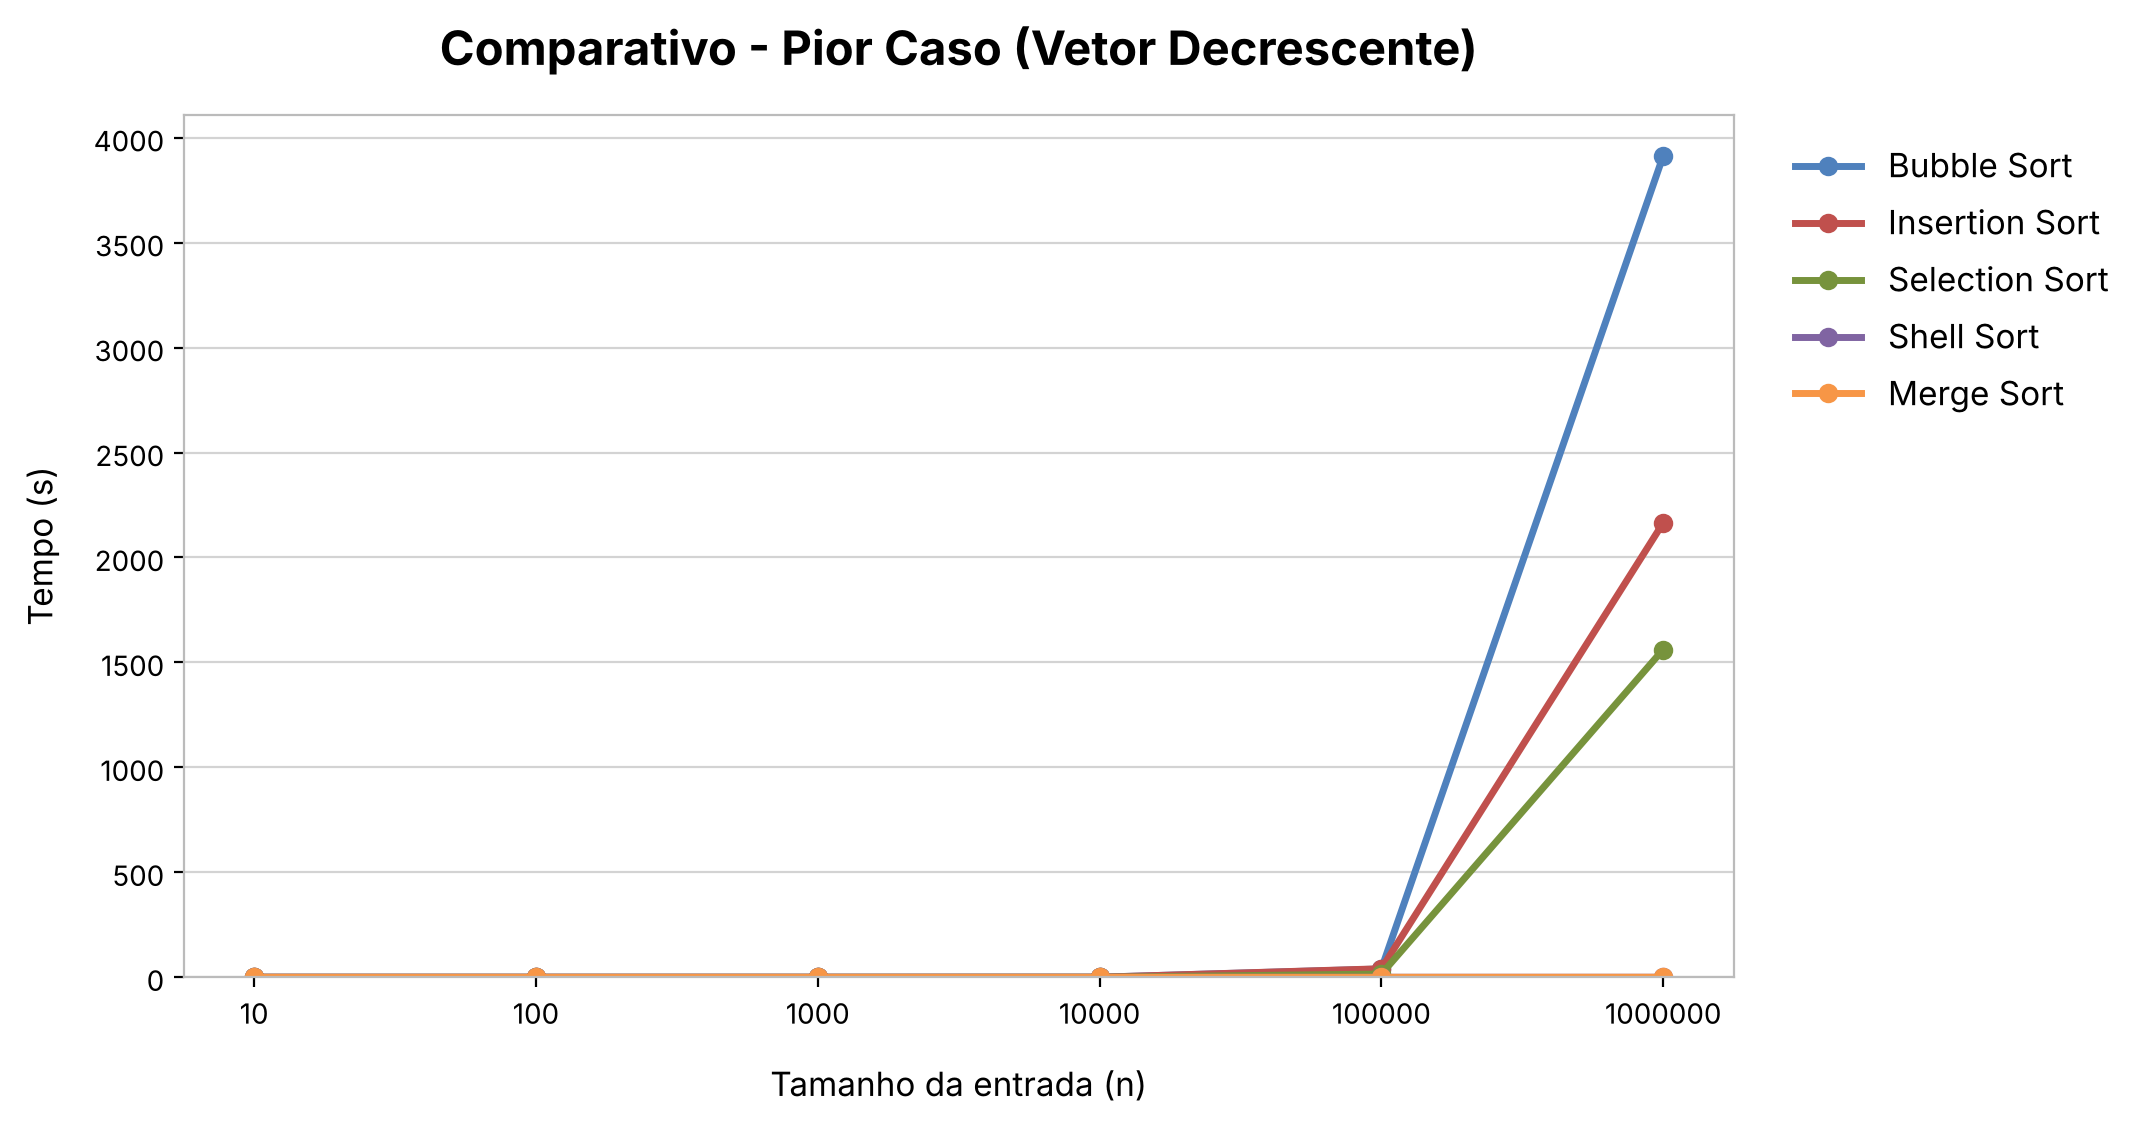
\includegraphics[width=0.8\textwidth]{Imagens/Geral/grafico_comp_piorcaso.png}
    \caption{Comparativo de Desempenho dos Algoritmos - Cenário Decrescente (elaborado pelo autor).}
    \label{fig:grafico_comp_pior}
\end{figure}

\FloatBarrier

\paragraph{Cenário Randômico (Caso Médio)}
A Figura \ref{fig:tabela_comp_medio} e a Figura \ref{fig:grafico_comp_medio} representam o cenário de uso mais comum e consolidam as observações anteriores. O \textbf{Merge Sort} se firma como a escolha superior, com apenas 0,292 segundo, seguido pelo \textbf{Shell Sort}, com 0,461 segundo. Este é o único cenário em que o \textit{Merge Sort} supera o \textit{Shell Sort}, pois o \textit{Shell Sort} depende da ordem dos dados e perde parte da vantagem quando eles estão desordenados. No grupo dos quadráticos, o \textbf{Insertion Sort} (1.086,290s) é o mais rápido, seguido pelo \textbf{Selection Sort} (1.658,270s) e, por último, pelo \textbf{Bubble Sort} (3.954,730s). O tempo do \textit{Insertion Sort} corresponde a aproximadamente metade do registrado em seu pior caso, comportamento coerente com a expectativa teórica de que, em média, cada elemento percorre metade da distância até sua posição final. Comparados ao \textit{Merge Sort}, o \textit{Insertion Sort} foi cerca de 3.700 vezes mais lento, o \textit{Selection Sort} cerca de 5.700 vezes e o \textit{Bubble Sort} cerca de 13.500 vezes.

\begin{figure}[!htb]
    \centering
    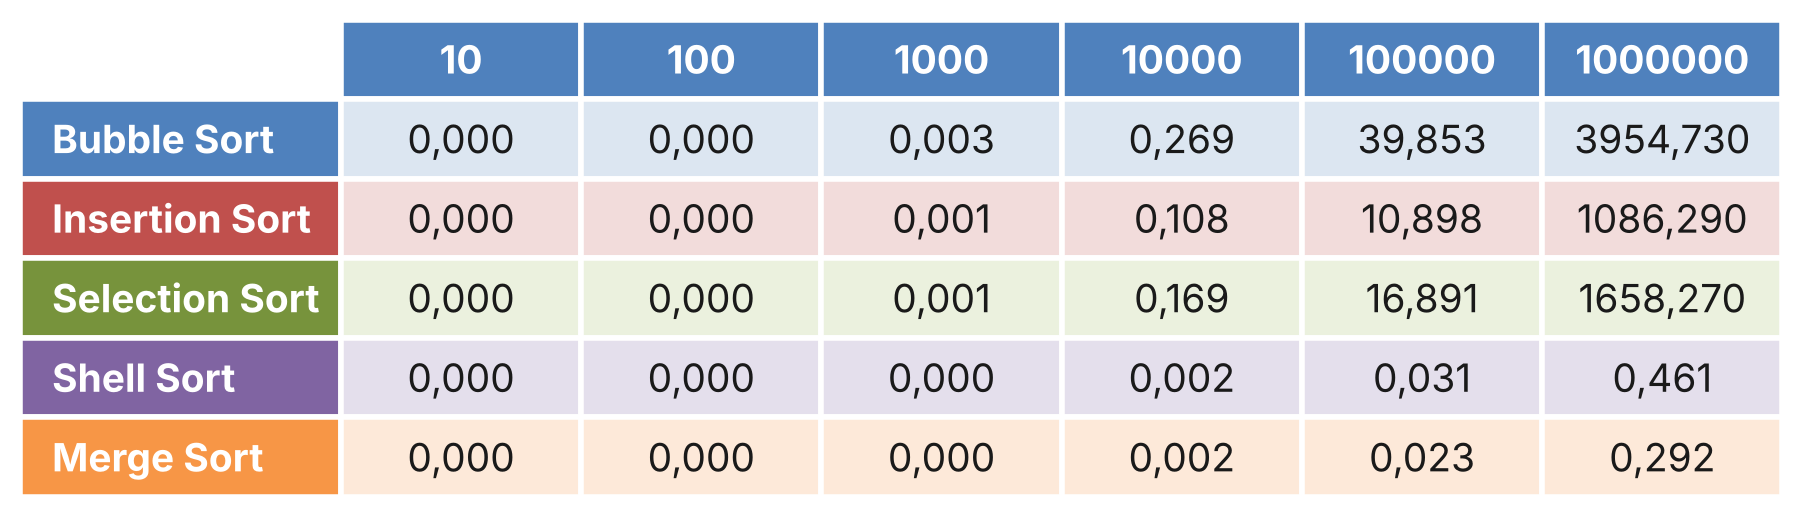
\includegraphics[width=0.8\textwidth]{Imagens/Geral/tabela_comp_casomedio.png}
    \caption{Tempos de execução (em segundos) dos cinco algoritmos - Cenário Randômico (elaborado pelo autor).}
    \label{fig:tabela_comp_medio}

    \vspace{0.5cm}

    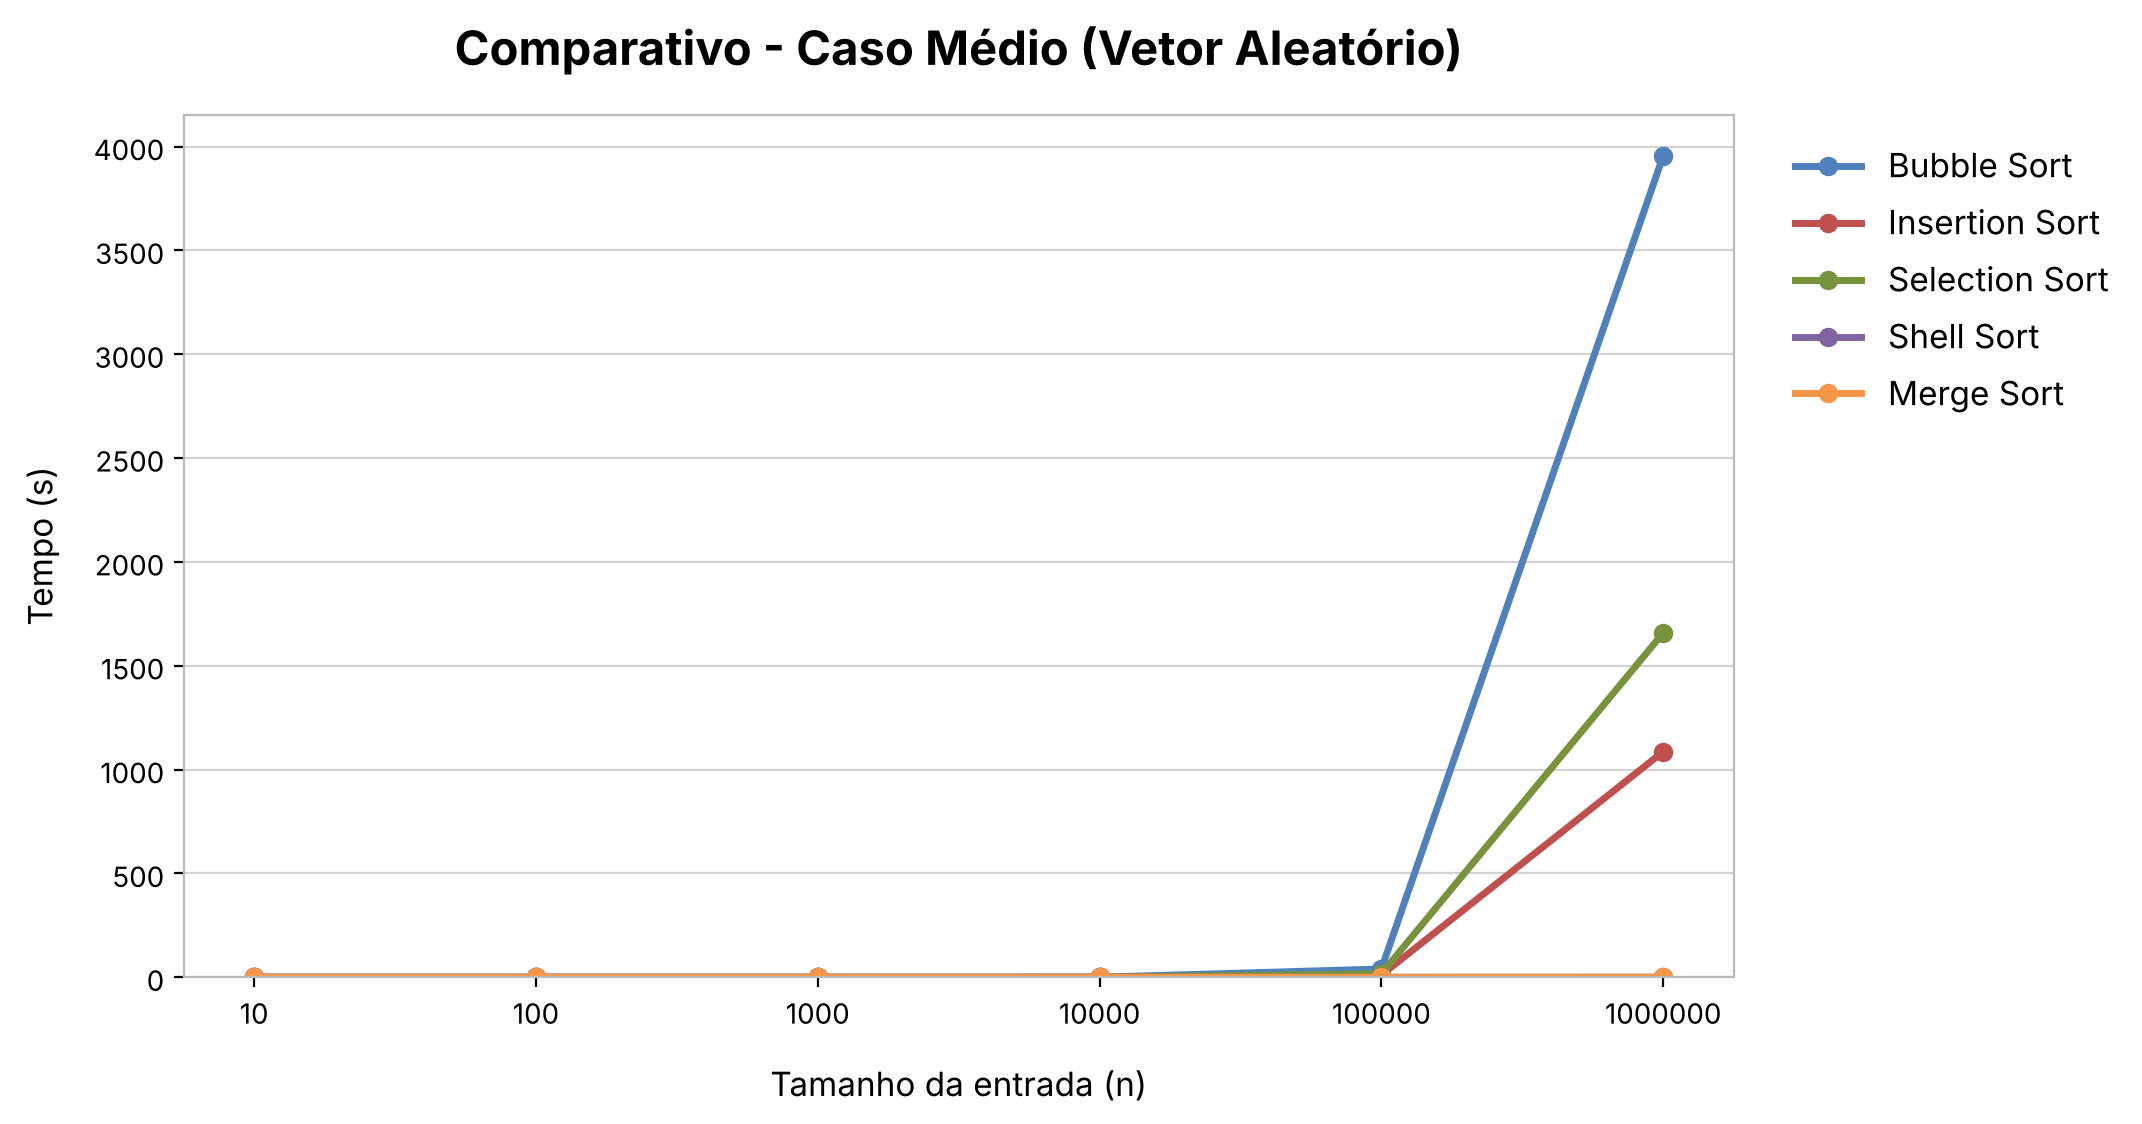
\includegraphics[width=0.8\textwidth]{Imagens/Geral/grafico_comp_casomedio.png}
    \caption{Comparativo de Desempenho dos Algoritmos - Cenário Randômico (elaborado pelo autor).}
    \label{fig:grafico_comp_medio}
\end{figure}

\FloatBarrier

\subsubsection*{Síntese da Análise Comparativa}

\qquad A análise conjunta dos três cenários permite dividir os algoritmos em duas categorias de desempenho. Os de complexidade $O(n^2)$ (\textit{Bubble}, \textit{Insertion} e \textit{Selection}) são adequados apenas para fins didáticos ou para entradas pequenas, tendo levado mais de vinte minutos para ordenar um milhão de elementos na maioria dos cenários. O \textit{Shell Sort}, com complexidade subquadrática, e o \textit{Merge Sort}, com complexidade $O(n \log n)$ em todos os casos, concluíram a mesma tarefa em menos de meio segundo em qualquer cenário.

\qquad Entre os quadráticos, cada um apresenta uma característica distinta. O \textit{Insertion Sort} é o mais sensível à ordem da entrada, variando de 0,005s a 2.164,840s entre o melhor e o pior caso, o que o torna a melhor opção quando há expectativa de dados parcialmente ordenados. O \textit{Selection Sort} é o mais previsível, com variação de apenas 21\% entre os cenários, sendo preferível quando o custo de cada troca é elevado. O \textit{Bubble Sort} não apresentou vantagem em nenhum cenário, tendo sido o mais lento nas entradas decrescente e aleatória.

\qquad Entre os dois algoritmos mais rápidos, a escolha depende do tipo de entrada e dos recursos disponíveis. O \textit{Shell Sort} foi mais rápido nos cenários crescente e decrescente, pois aproveita a ordem prévia dos dados, e funciona \textit{in-place}, sem memória adicional. O \textit{Merge Sort} foi o mais rápido no cenário aleatório e manteve desempenho regular, variando de 0,155s a 0,292s entre os cenários, mas exige um vetor auxiliar de tamanho $n$. Além disso, é estável, o que o torna preferível quando se deseja preservar a ordem relativa de elementos iguais.

\qquad Vale registrar que, para entradas de até 1.000 elementos, os cinco algoritmos concluíram a ordenação em menos de 0,005 segundo, tornando a escolha irrelevante nessa faixa. A diferença entre eles só se torna determinante a partir de dezenas de milhares de elementos, o que reforça a importância de considerar a escala do problema ao selecionar um algoritmo de ordenação.

\FloatBarrier
		\newpage
  
		\section{CONCLUSÃO}
		% --- Conteúdo para conclusao.tex ---

\qquad Este trabalho analisou cinco algoritmos de ordenação sob três cenários de entrada, confrontando a análise teórica de complexidade com os tempos obtidos experimentalmente. Os resultados confirmaram o comportamento previsto pela teoria e evidenciaram o impacto prático da escolha do algoritmo em aplicações que lidam com grandes volumes de dados.

\qquad A principal constatação diz respeito à separação entre os algoritmos quadráticos e os mais eficientes, \textit{Shell Sort} e \textit{Merge Sort}. Enquanto \textit{Bubble Sort}, \textit{Insertion Sort} e \textit{Selection Sort} levaram entre 18 e 66 minutos para ordenar um milhão de elementos aleatórios, o \textit{Shell Sort} concluiu a mesma tarefa em 0,461 segundo e o \textit{Merge Sort} em 0,292 segundo. Essa diferença não decorre de otimizações no código, e sim da ordem de complexidade de cada método: o ganho obtido ao substituir um algoritmo $O(n^2)$ por um subquadrático ou $O(n \log n)$ supera, em larga escala, qualquer ajuste pontual de implementação.

\qquad O \textit{Merge Sort} foi o único algoritmo recursivo do trabalho e o único baseado na estratégia de dividir para conquistar. A resolução de sua recorrência resultou em $T(n) = n + n \log_2 n$, ou seja, $O(n \log n)$ nos três casos, e os tempos medidos confirmaram essa previsão: ao aumentar a entrada de 100.000 para 1.000.000 de elementos, o tempo do caso aleatório cresceu cerca de 12,7 vezes, valor próximo das 12 vezes esperadas para $n \log n$. Também ficou evidente que sua eficiência tem um custo, pois ele exige um vetor auxiliar de tamanho $n$, enquanto os demais algoritmos ordenam o vetor \textit{in-place}.

\qquad A comparação entre os dois algoritmos mais rápidos mostrou que não existe um vencedor absoluto. O \textit{Merge Sort} foi o mais rápido com entrada aleatória e apresentou tempos parecidos em todos os cenários, já que realiza o mesmo trabalho em qualquer ordem dos dados. O \textit{Shell Sort}, por outro lado, foi mais rápido nas entradas crescente e decrescente, pois aproveita a organização prévia do vetor, e não utiliza memória adicional. A escolha entre eles depende, portanto, do tipo de dado esperado e da memória disponível.

\qquad Os testes também mostraram que a ordem inicial dos dados afeta cada algoritmo quadrático de maneira distinta. O \textit{Insertion Sort} foi o mais sensível, variando de 0,005 segundo no melhor caso a 2.164,840 segundos no pior, diferença de mais de quatrocentas mil vezes, o que o torna vantajoso quando há expectativa de dados parcialmente ordenados. O \textit{Selection Sort} apresentou o comportamento mais previsível entre os quadráticos, com variação de apenas 21\% entre os cenários. Já o \textit{Bubble Sort} não obteve vantagem em nenhum cenário, tendo registrado o pior desempenho nas entradas decrescente e aleatória.

\qquad Um resultado que merece registro é o fato de o \textit{Bubble Sort} ter sido ligeiramente mais lento com entrada aleatória do que com entrada decrescente, contrariando à primeira vista a expectativa teórica de pior caso. A análise dessa ocorrência mostrou que, na implementação utilizada, o número de comparações é idêntico nos três cenários, variando apenas o número de trocas e o padrão de acesso à memória. Isso reforça que a análise assintótica descreve a tendência de crescimento do algoritmo, e não o tempo exato de execução, que depende também de fatores de hardware.

\qquad Observou-se ainda que, para entradas de até 1.000 elementos, os cinco algoritmos concluíram a ordenação em tempo inferior a 0,005 segundo, faixa em que a escolha entre eles é irrelevante. As diferenças só passam a ser determinantes a partir de dezenas de milhares de elementos, o que indica que a seleção de um algoritmo deve considerar a escala esperada do problema, e não apenas sua classificação teórica.

\qquad Por fim, o trabalho permitiu articular os conteúdos de análise de complexidade com a prática de implementação e medição. A construção das tabelas de custo, dos testes de mesa, da recorrência do \textit{Merge Sort} e das funções de tempo para cada cenário tornou possível prever o comportamento dos algoritmos antes mesmo da execução, e os resultados experimentais confirmaram essas previsões. Como continuidade natural do estudo, seria pertinente incluir o \textit{Quick Sort}, avaliar versões otimizadas do \textit{Merge Sort}, como o uso do \textit{Insertion Sort} em trechos pequenos, e testar o efeito de diferentes sequências de \textit{gaps} sobre o desempenho do \textit{Shell Sort}.
		\newpage
  
		\section{REFERÊNCIAS BIBLIOGRÁFICAS}
		\begingroup
\renewcommand{\refname}{}
\vspace{-2.5em}
\begin{thebibliography}{3}

\bibitem{cormen}
CORMEN, Thomas H.; LEISERSON, Charles E.; RIVEST, Ronald L.; STEIN, Clifford. \textit{Algoritmos: teoria e prática}. 3. ed. Rio de Janeiro: Elsevier, 2012.

\bibitem{knuth}
KNUTH, Donald E. \textit{The Art of Computer Programming, Volume 3: Sorting and Searching}. 2. ed. Boston: Addison-Wesley, 1998.

\bibitem{sedgewick}
SEDGEWICK, Robert; WAYNE, Kevin. \textit{Algorithms}. 4. ed. Boston: Addison-Wesley, 2011.

\end{thebibliography}
\endgroup
		\newpage
\end{document}